    \documentclass[a4paper,12pt,twoside]{ThesisStyle}
\usepackage[utf8]{inputenc}
\usepackage{thesis-style}
\usepackage[english]{babel}
\usepackage[T1]{fontenc}

\usepackage{subcaption}
\usepackage{graphicx}
\usepackage{enumitem} % Required for customizing itemize labels
\usepackage{enumitem}
\usepackage{fancyvrb}
\usepackage[toc,page]{appendix}
\usepackage{adjustbox}
\usepackage{pdflscape}
\usepackage{booktabs}% http://ctan.org/pkg/booktabs



\usepackage[table]{xcolor}
\definecolor{signaturegray}{gray}{0.98}

\RequirePackage{tikz}
\definecolor{ao}{rgb}{0.0, 0.5, 0.0}
\definecolor{darkpastelgreen}{rgb}{0.01, 0.75, 0.24}
\definecolor{amber}{rgb}{1.0, 0.75, 0.0}
\usetikzlibrary{mindmap}  % Mindmap drawing library

\setlength{\parindent}{0pt} % Drops all identation of all paragraphs

\begin{document}

\frontmatter

\pagenumbering{gobble}

\thispagestyle{empty}
\begin{table}[htb]
\centering
\begin{Large}
\resizebox{\textwidth}{!}{\begin{tabular}{ | l |}
 \hline
 \\

\includegraphics[scale=0.9]{imatges/logo_eps.png} \\[0.7cm]
\centerline{Treball Final de Màster}\\[1cm]
\hline
\\
Estudi: Màster en Ciència de Dades\\[0.7cm]
\hline
\\
Títol: Una Plataforma per Classificar Melanomes \\[0.7cm]
\hline
\\
Document: Memòria\\[0.7cm]
\hline
\\
Alumne: Wilber Eduardo Bermeo Quito \\[0.7cm]
\hline
\\
Tutor: Rafael Garcia Campos \\
Departament:  ARQUITECTURA I TECNOLOGIA DE COMPUTADORS \\
Àrea: ARQUITECTURA I TECNOLOGIA DE COMPUTADORS \\[0.7cm]
\hline
\\
Convocatòria (mes/any): Setembre 2022\\[0.7cm]
\hline

\end{tabular}}
\end{Large}
\end{table}

\newpage
\hypersetup{pageanchor=false}
\begin{titlepage}

% Upper part of the page

\includegraphics[scale=0.9]{imatges/logo_eps.png} \\[1cm]
\begin{center}
\textsc{\Large Master's thesis} \\[1cm]

% Title
\begin{spacing}{2}
\HRule \\
\textbf{\Huge A Platform for Classifying Melanoma} \\
\HRule \\[0.5cm]
\end{spacing}

% Author and supervisor and other data
{
\large
\textsc{Wilber Eduardo Bermeo Quito} \\
\small{September 2022} \\[0.75cm]
Master in Data Science \\[0.75cm]
\emph{Advisors:} \\[0.1cm]
\large
\textsc{Dr. Rafael Garcia Campos} \\
\small{Universitat de Girona} \\
\small{Departament of Computer Architecture and Technology} \\[0.5cm]

\large
\textsc{Sr. Luis Pla Llopis} \\
\small{Accenture S.L.} \\

}

\end{center}
\end{titlepage}
\hypersetup{pageanchor=true}

\titlepage

%\dominitoc


\pagenumbering{roman}

\chapter*{Summary}
%\label{cap:resum}

\chapter*{Gratitudes}
%\label{cap:agraiments}

Per començar vull agrair molt especialment a \ldots


\tableofcontents

\listoffigures

\listoftables

\mainmatter

\chapter{Introduction}
\label{cap:intro}

\section{Problem Statement}

Skin cancer, including melanoma, represents a significant public health concern
worldwide. Melanoma, in particular, poses a considerable challenge due to its
high mortality rate and the need for early detection for successful treatment.
Early and correct diagnosis is key for ensuring patients have the best possible
prognosis. Melanoma misdiagnosis accounts for more pathology and dermatology
malpractice claims than any cancer other than breast cancer, as an early
misdiagnosis can significantly reduce a patient’s chances of survival
\cite{Melanoma}. \newline

Dermoscopy, also known as dermatoscopy Figure
\ref{fig:procedure_dermoscopy}, is a noninvasive technique widely utilized for
the examination of cutaneous lesions. It involves the use of a handheld
instrument called a dermatoscope to visualize subsurface skin structures that
are typically not visible to the naked eye. The dermatoscope illuminates the
skin surface and provides magnification, allowing for a detailed examination of
the epidermis, the dermoepidermal junction, and the papillary dermis. By
analyzing these structures, dermatologists can identify specific features and
patterns associated with various skin conditions, including melanoma
\cite{Dermoscopy}.

\begin{figure}[htb] \centering
  
\includegraphics[width=6.5 cm]{imatges/introduction/medical_procedure_dermastocopy.jpeg}
  \caption[Dermoscopy Procedure]{\textit{Dermoscopy Procedure. Illustration by MD Anderson Cancer Center}}
  {\label{fig:procedure_dermoscopy}}
\end{figure}

Worldwide, in 2020 an estimated 324,635 people were diagnosed with melanoma and
an estimated 57,043 people worldwide died from melanoma the same year
\cite{CancerStats}. The introduction of sophisticated machinery to take high
quality dermoscopy images (Figure \ref{fig:subset_isic}) and new
techniques in dermoscopy procedures seems not enough to fight against
melanoma, but the developments in artificial intelligence (AI) especially in
deep learning techniques, have made Computer-Aided Diagnosis
(CAD)\footnote{Computer-Aided Diagnosis (CAD) refers to the use of computer
algorithms and technologies to assist healthcare professionals in the process
of medical diagnosis} a promising path towards medical automation.

\begin{figure}[h!] \centering
  \begin{subfigure}{0.3\textwidth}
    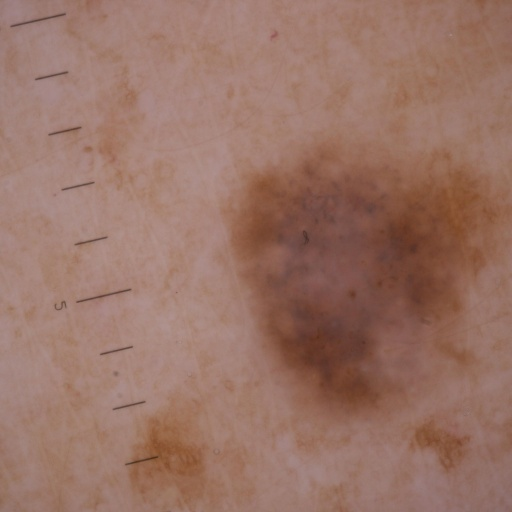
\includegraphics[width=\textwidth]{imatges/introduction/subset_isic/ISIC_1752943.jpg}
  \end{subfigure}
  \hfill
  \begin{subfigure}{0.3\textwidth}
    
\includegraphics[width=\textwidth]{imatges/introduction/subset_isic/ISIC_1766619.jpg}
  \end{subfigure}
  \hfill
  \begin{subfigure}{0.3\textwidth}
    
\includegraphics[width=\textwidth]{imatges/introduction/subset_isic/ISIC_1448526.jpg}
  \end{subfigure}
  \caption[Dermoscopy Images]{\textit{Dermoscopy Images. Illustration by ISIC Archive}}
  \label{fig:subset_isic}
\end{figure}

However, there are several limitations that raise doubts about the
effectiveness of automated melanoma cancer classifiers and their suitability
for integration into the medical system. Firstly, certain methods are
constructed based on theoretical models of melanoma appearance, which may
restrict their applicability to specific morphologies and fail to capture the
wide range of variations seen in real-world scenarios. Secondly, AI systems
utilized in these classifiers are trained to address a singular and narrow
task. Unlike human dermatologists, these systems lack the ability to consider
holistic patient information when formulating a final diagnosis, reflecting the
concept of weak AI \cite{WeakAI}. Lastly, numerous methods have been trained
and evaluated using high-quality image frames, which may result in instability
when applied under real-time visibility conditions where image quality is often
compromised. A fundamental part of machine learning is the problem of
generalization, that is, how to make sure that a trained model performs well on
unseen data. If the unseen data has different distribution, i.e. a domain shift
exists, the problem is significantly more difficult even the smallest changes
in the statistics as compared to the training data can cause a deep neural
network to fail completely \cite{DomainShift}. \newline

Addressing these limitations and developing melanoma cancer classifiers that
encompass a wider range of morphologies, incorporate holistic patient
information, consider relevant elements, and demonstrate robustness in
real-world scenarios are crucial for improving the reliability and
effectiveness of melanoma detection and diagnosis systems. \newline

\section{Project Objectives}

The main objective of this project is to create a health care infrastructure,
focused on melanoma detection using deep learning methods to train a system
capable of detecting melanoma on dermoscopy images to test the ability of
computer-assisted image analysis. To this end, the gradual achievements that
must be accomplished are:

\begin{itemize}
  \item Gaining a comprehensive understanding of the theory behind deep learning and its practical applications.
  \item Analyzing images from dermostocopy and understanding its most important features.
  \item Train deep learning models with different techniques based on tranfer-learning focused on the images of the melanoma ISIC Challenge \cite{IsicChallenge}.
  \item Developing a CAD infrastructure. The CAD infrastructure contains the
    already trained models with a simple web UI\footnote{The user interface
    (UI) is the point of human-computer interaction and communication in a
    device} an API\footnote{API stands for Application Programming Interface}
    and finally a mechanism using Docker to create the images of the services
    making it ease to deploy in any based Linux System.
\end{itemize}

\section{Personal Motivation}

I envisioned this project as a unique fusion of three personal passions.
Firstly, I was fueled by a deep fascination with human cognition and reasoning.
Machines, in my eyes, represented a novel paradigm through which I could delve
further into this captivating realm. \newline

I am also motivated by the remarkable problem-solving capacity of data.
Regardless of its structure, data holds immense potential to uncover hidden
patterns, provide insights, and drive innovation. The ability to extract
meaningful information from data, regardless of its form, inspires me to
constantly expand my knowledge and skills in order to contribute to the field
of data science and make a tangible difference in the world. \newline

Last but not least, I am driven by the immense power of automation and its
ability to democratize access to research knowledge. I am amazed by how
automation processes can extract value and make them readily available to
professionals and the public alike.

\section{Statement of Originality}

I, Wilber Eduardo Bermeo Quito, declare that the thesis titled "A Platform for
Classifying Melanoma" is an original work completed with the support and
collaboration of Accenture SL and the VICOROB laboratory. \newline

The content presented in this thesis is the outcome of my independent research
efforts, guided by the knowledge and expertise acquired through my academic
studies and the valuable contributions from Accenture S.L and the VICOROB
laboratory. \newline

I acknowledge the importance of academic integrity and the consequences of
plagiarism. Hence, I affirm that all the information, data, results, figures,
and conclusions presented in this thesis are authentic and original. Any
references or sources used have been appropriately cited and referenced.

\section{Regulatory Framework}

The inclusion of legal considerations has become a significant aspect of the
field of medical imaging. Privacy concerns and the potential misuse of personal
information make sharing and distributing medical data particularly
challenging. To address these limitations, recent research collaborations have
focused on promoting the sharing of patient data through de-identification
methods. However, it is crucial to thoroughly analyze the obligations related
to the protection of individuals and their personal data before engaging in
projects involving medical imaging. \newline

When working with medical images, it is the utmost importance to prioritize
patient privacy rights. In the context of developing a skin lesions database,
it is necessary to obtain signed consent from patients for the publication of
their data. For this thesis, the ISIC Archive database was utilized, this
database serves as a publicly accessible resource for teaching, research, and
the development and testing of diagnostic artificial intelligence algorithms,
and it resolves any concerns related to consent \cite{IsicArchive}. It is a
large and continually expanding open-source archive of skin images.

\section{Related Work}

Melanoma Computer-Aided Diagnosis (CAD) classifiers have been a subject of extensive research and development in recent years,
also there has been a lot of work in platforms capable of explaining the way
these models infer. Bellow is mentioned remarkable related work to the subject.
\newline

\vspace{0.5cm}
\textbf{Identifying Melanoma Images using EfficientNet Ensemble: Winning Solution to the SIIM-ISIC Melanoma Classification Challenge} \newline

Winning solution to the SIIM-ISIC Melanoma Classification Challenge. It is an
ensemble of convolutions of neural network (CNN) models with different
backbones and input sizes \cite{WinningISIC}.  \newline

\vspace{0.5cm} \textbf{Dermatologist-level classification of skin cancer with
deep neural networks} \newline

This study demonstrated the use of a deep learning algorithm to classify skin
lesions, including melanoma, with accuracy comparable to dermatologists. The
deep neural network was trained on a large dataset of images and achieved high
sensitivity and specificity \cite{SkinCancerDeepNN}. \newline

\vspace{0.5cm} \textbf{Computerized analysis of pigmented skin lesions: A
review}  \newline

The goal of this paper is to give a detailed explanation and clear up any
confusion about the words and phrases used in melanoma studies. And to organize
and group together useful sources, making it easier to find information on a
particular sub-topic when searching through the existing literature
\cite{MelanomaTopicsReview}. \newline

\newpage

\vspace{0.5cm}
\textbf{CNN-Explainer} \newline

The CNN-Explainer is an interactive web-based tool that aims to provide
explanations for the predictions made by convolutional neural network (CNN)
models \cite{CNNExplainer}.

\section{Contribution to Melanoma Detection}

In this section, we present the contribution to the field of melanoma detection
through the development of a melanoma CAD (Computer-Aided Diagnosis)
infrastructure classifier. \newline

The thesis comprises multiple models employing various techniques, including
transfer learning, data augmentation, just-in-time testing, regularization, and
others. To compare these models, tools like W\&B (Weight \& Biases), a MLOps
platform for experiment tracking, and MLXTEND, providing utilities and
extensions for machine learning and data science in Python's scientific
computing stack, were utilized. The experiments were conducted using the ISIC
Archive dataset, consisting of benign and malignant skin lesions. Prior to
analysis, the dataset underwent preprocessing to enhance quality and normalize
features. Consequently, accurate classification and differentiation of melanoma
lesions from benign ones were achieved. \newline

In order to to ensure the usability of the trained models,
two services were developed. These services include a user-friendly UI and an
API, both of which were containerized using Docker technology. By
containerizing the UI, an intuitive and interactive user experience was
provided, enabling users to seamlessly interact with the melanoma CAD system.
Similarly, containerizing the API streamlined request handling and prediction
serving, resulting in efficient performance. This approach facilitated easy
deployment across various platforms.


\chapter{Related Work and State of the Art}
\label{cap:estat}

Melanoma, a type of cancer that arises from melanin-producing cells, can be
found in various parts of the body such as the skin, eyes, nerve centers, and
meninges. Early diagnosis is crucial for improving the chances of curing
melanoma, even though it has the highest increasing incidence rate among all
skin cancer types. According to a study \cite{TimelyMelanomaDetection}, timely
identification of early-stage skin cancer resulted in a significant 90\%
reduction in mortality rates. For instance, patients diagnosed with stage I
melanoma have a 10-year overall survival probability ranging from 94\% to 98\%,
while those in stage IV have a much lower estimated 10-year overall survival
rate of just 10\% to 15\%. \\

Dermoscopy is a non-surgical method used to examine the underlying layers of
the skin. While it can yield good results, it requires extensive training and
experience in dermatology. However, it may not provide a definitive diagnosis
for melanoma, especially in its early stages. Consequently, there is a need for
an automated diagnostic tool. \\

In \cite{EpidemiologySkinCancer} study, the melanoma task classification was
compared between expert opinions and artificial neural networks. The computer
program demonstrated had an area under the receiver operating characteristic
curve of 0.87, which was higher than the dermatologists (0.74), the program
also had a higher sensitivity in classification of 85\% against the 76\% by the
dermatologists. These findings indicate the potential utilization of automated
systems in the field of skin cancer detection. \\

For cancer prediction, a supervised learning approach is employed. The most
common algorithms or methodologies include decision trees, convolutional neural
networks (CNN), support vector machines (SVM), k-nearest neighbors (KNN) and
Transformers. One of the most powerful systems are CNNs (Convolutional Neural
Networks), despite the fact that their use may involve a loss of
explainability, which is a major concern in healthcare systems. \\

Although this project goes beyond the mere creation of highly accurate models
for classifying melanoma, we have taken into consideration and reviewed related
works that have influenced and guided our own path.

\section{Identifying Melanoma Images Using EfficientNet Ensemble}

The winning approach to the 2020 SIIM-ISIC Melanoma Classification Challenge
\cite{ISICKaggle}. The team not only let the competition source code available
on GitHub \cite{WinningISICGithub} but they also wrote a paper explaining in
detail their investigation \cite{WinningISIC}. \\

The SIIM-ISIC Melanoma Classification Challenge was conquered by this ensemble of
convolutional neural networks (CNN). The winning solution involved training 16
EfficientNets, along with a ResNext101 and a ResNet101. To create this ensemble
of models, various strategies were employed, including utilizing patients'
metadata in addition to dermoscopy images, training models with different input
image sizes, and even training the models for varying numbers of epochs
\cite{WinningISIC}.

\begin{itemize}
  \item Implementation of a stable validation scheme.
  \item Effective selection of the model target.
  \item Thoughtful optimization of the pipeline.
  \item Utilization of ensemble learning with highly diverse models.
\end{itemize}

The submission that won achieved an AUC (Area Under the Curve)\footnote{AUC is
a metric that quantifies the overall quality of a binary classification model
by measuring the area under its ROC curve. It provides a single value that
summarizes the model's ability to discriminate between positive and negative
instances.} score of 0.9600 on cross-validation and 0.9490 on the private
leaderboard. \\

From their work, we adopted various deep learning techniques. For instance, we
applied the same way they evaluate models given an unbalanced multi-class
data-sets like as the ISIC dataset is. To properly assess the training process,
they utilized the AUC with one-vs-rest (OvR) metric. This project as well uses
this metric to evaluate the performance of the models. \\

Another aspect the current thesis borrowed from this work is the approach to
cleaning and mapping data-sets from different years. They trained their models
with different input image sizes, but the process of mapping and joining the
data-sets into a single data-set was similar to our approach, where we
consistently mapped the data into eight different classes. \\

The pipeline of data augmentation that is implemented in the work is also
reused. Equivalent to them, this thesis uses {\tt
albumentations}\cite{Albumentations} library instead of the native data
agumentation package provided from PyTorch. \\

These inspirations and adaptations from the related work has greatly influenced
the development and organization of this deep learning project.

\section{CNN Explainer}

CNN explainer is a web page created through a collaborative research effort
between Georgia Tech and Oregon State\cite{CNNExplainer}. It leverages
TensorFlow.js, a deep learning library that utilizes GPU acceleration within
the web browser, to load pretrained models for visualization. The entire
interactive system is implemented in JavaScript, utilizing Svelte as a
framework and D3.js for visualizations. With CNN Explainer, users can upload
images and obtain predictions for those images across ten different classes.
\\

While CNN Explainer primarily aims to serve educational purposes, the UI of the
current thesis, focuses on providing dermoscopy images predictions and
information about the models used and their outputs. The inspiration for
incorporating an interactive UI for end users stemmed from CNN Explainer.
Consequently, we utilized the same web framework to develop the UI.

\section{Dermatologist-level Classification of Skin Cancer with
Deep Neural Networks}

This study demonstrated the use of a deep learning algorithm to classify skin
lesions, including melanoma, with accuracy comparable to dermatologists. The
deep neural network was trained on a large dataset of images and achieved high
sensitivity and specificity \cite{SkinCancerDeepNN}.

\section{Computerized Analysis of Pigmented Skin Lesions: A
Review}

The goal of this paper is to review the papers on computerized analysis of
dermoscopy and clinical images of pigmented skin lesions. The paper also
clarifies terminology that is often misused in the literature, and it also
organizes and group together useful sources, making it easier to find
information on a particular sub-topic when searching through the existing
literature \cite{MelanomaTopicsReview}.


\chapter{Domain} \label{cap:problem_domain}

In this chapter, we will delve into the details of melanoma cancer, including
its origins, factors contributing to its development, and strategies to
minimize the risk of its occurrence. Additionally, we will explore other common
types of skin cancer and their underlying causes. \\

By the end of this chapter, our aim is to provide a comprehensive understanding
of this condition, equipping you with the knowledge necessary to comprehend the
proposed solution in this thesis.

\section{The Skin}

The skin, which is our body's largest organ \cite{BaseCancerKnowledge}, plays a
crucial role in safeguarding us against external threats and maintaining our
overall health. It consists of several layers (Figure
\ref{fig:melanoma_diagram}), with the main layers being:

\begin{itemize} \item \textbf{Epidermis}

      The epidermis is the outermost layer of the skin, serving as a protective
      shield against environmental factors. It consists mainly of flat,
      scale-like cells called keratinocytes. These cells produce a tough
      protein called keratin, which helps make the skin waterproof and
      resistant to damage. Within the epidermis, specialized cells called
      melanocytes produce melanin, the pigment responsible for skin color.
      Melanin also helps protect the skin from harmful ultraviolet (UV)
      radiation. \\

      The epidermis is made up of several layers, including the stratum
      corneum, the topmost layer composed of dead skin cells that are
      continuously shed and replaced by new cells from the lower layers. The
      epidermis also contains other types of cells, such as Langerhans cells,
      which are part of the immune system and help defend against infections.

      \newpage

    \item \textbf{Dermis}

      Beneath the epidermis lies the dermis, a complex layer that provides
      structural support to the skin. The dermis contains a network of blood
      vessels that supply nutrients and oxygen to the skin cells. It also
      houses various structures, including hair follicles, sweat glands,
      sebaceous glands, and nerve endings. The dermis is composed of collagen
      and elastin fibers, which give the skin its strength, elasticity, and
      flexibility. These fibers allow the skin to stretch and recoil as needed.
      The dermis also plays a crucial role in thermoregulation by regulating
      blood flow to control body temperature.

    \item \textbf{Hypodermis (Subcutaneous Tissue)}

      The deepest layer of the skin is called the hypodermis or subcutaneous
      tissue. It is primarily made up of adipose tissue, which provides
      insulation, cushioning, and energy storage. The hypodermis helps to
      regulate body temperature by acting as an insulating layer, preventing
      heat loss. It also acts as a shock absorber, protecting the underlying
      structures and organs from injury. Additionally, the hypodermis serves as
      a connection between the skin and the underlying muscles and bones. It
      contains blood vessels and nerve endings that supply nutrients and
      sensations to the skin.

\end{itemize}

\begin{figure}[H] \centering
  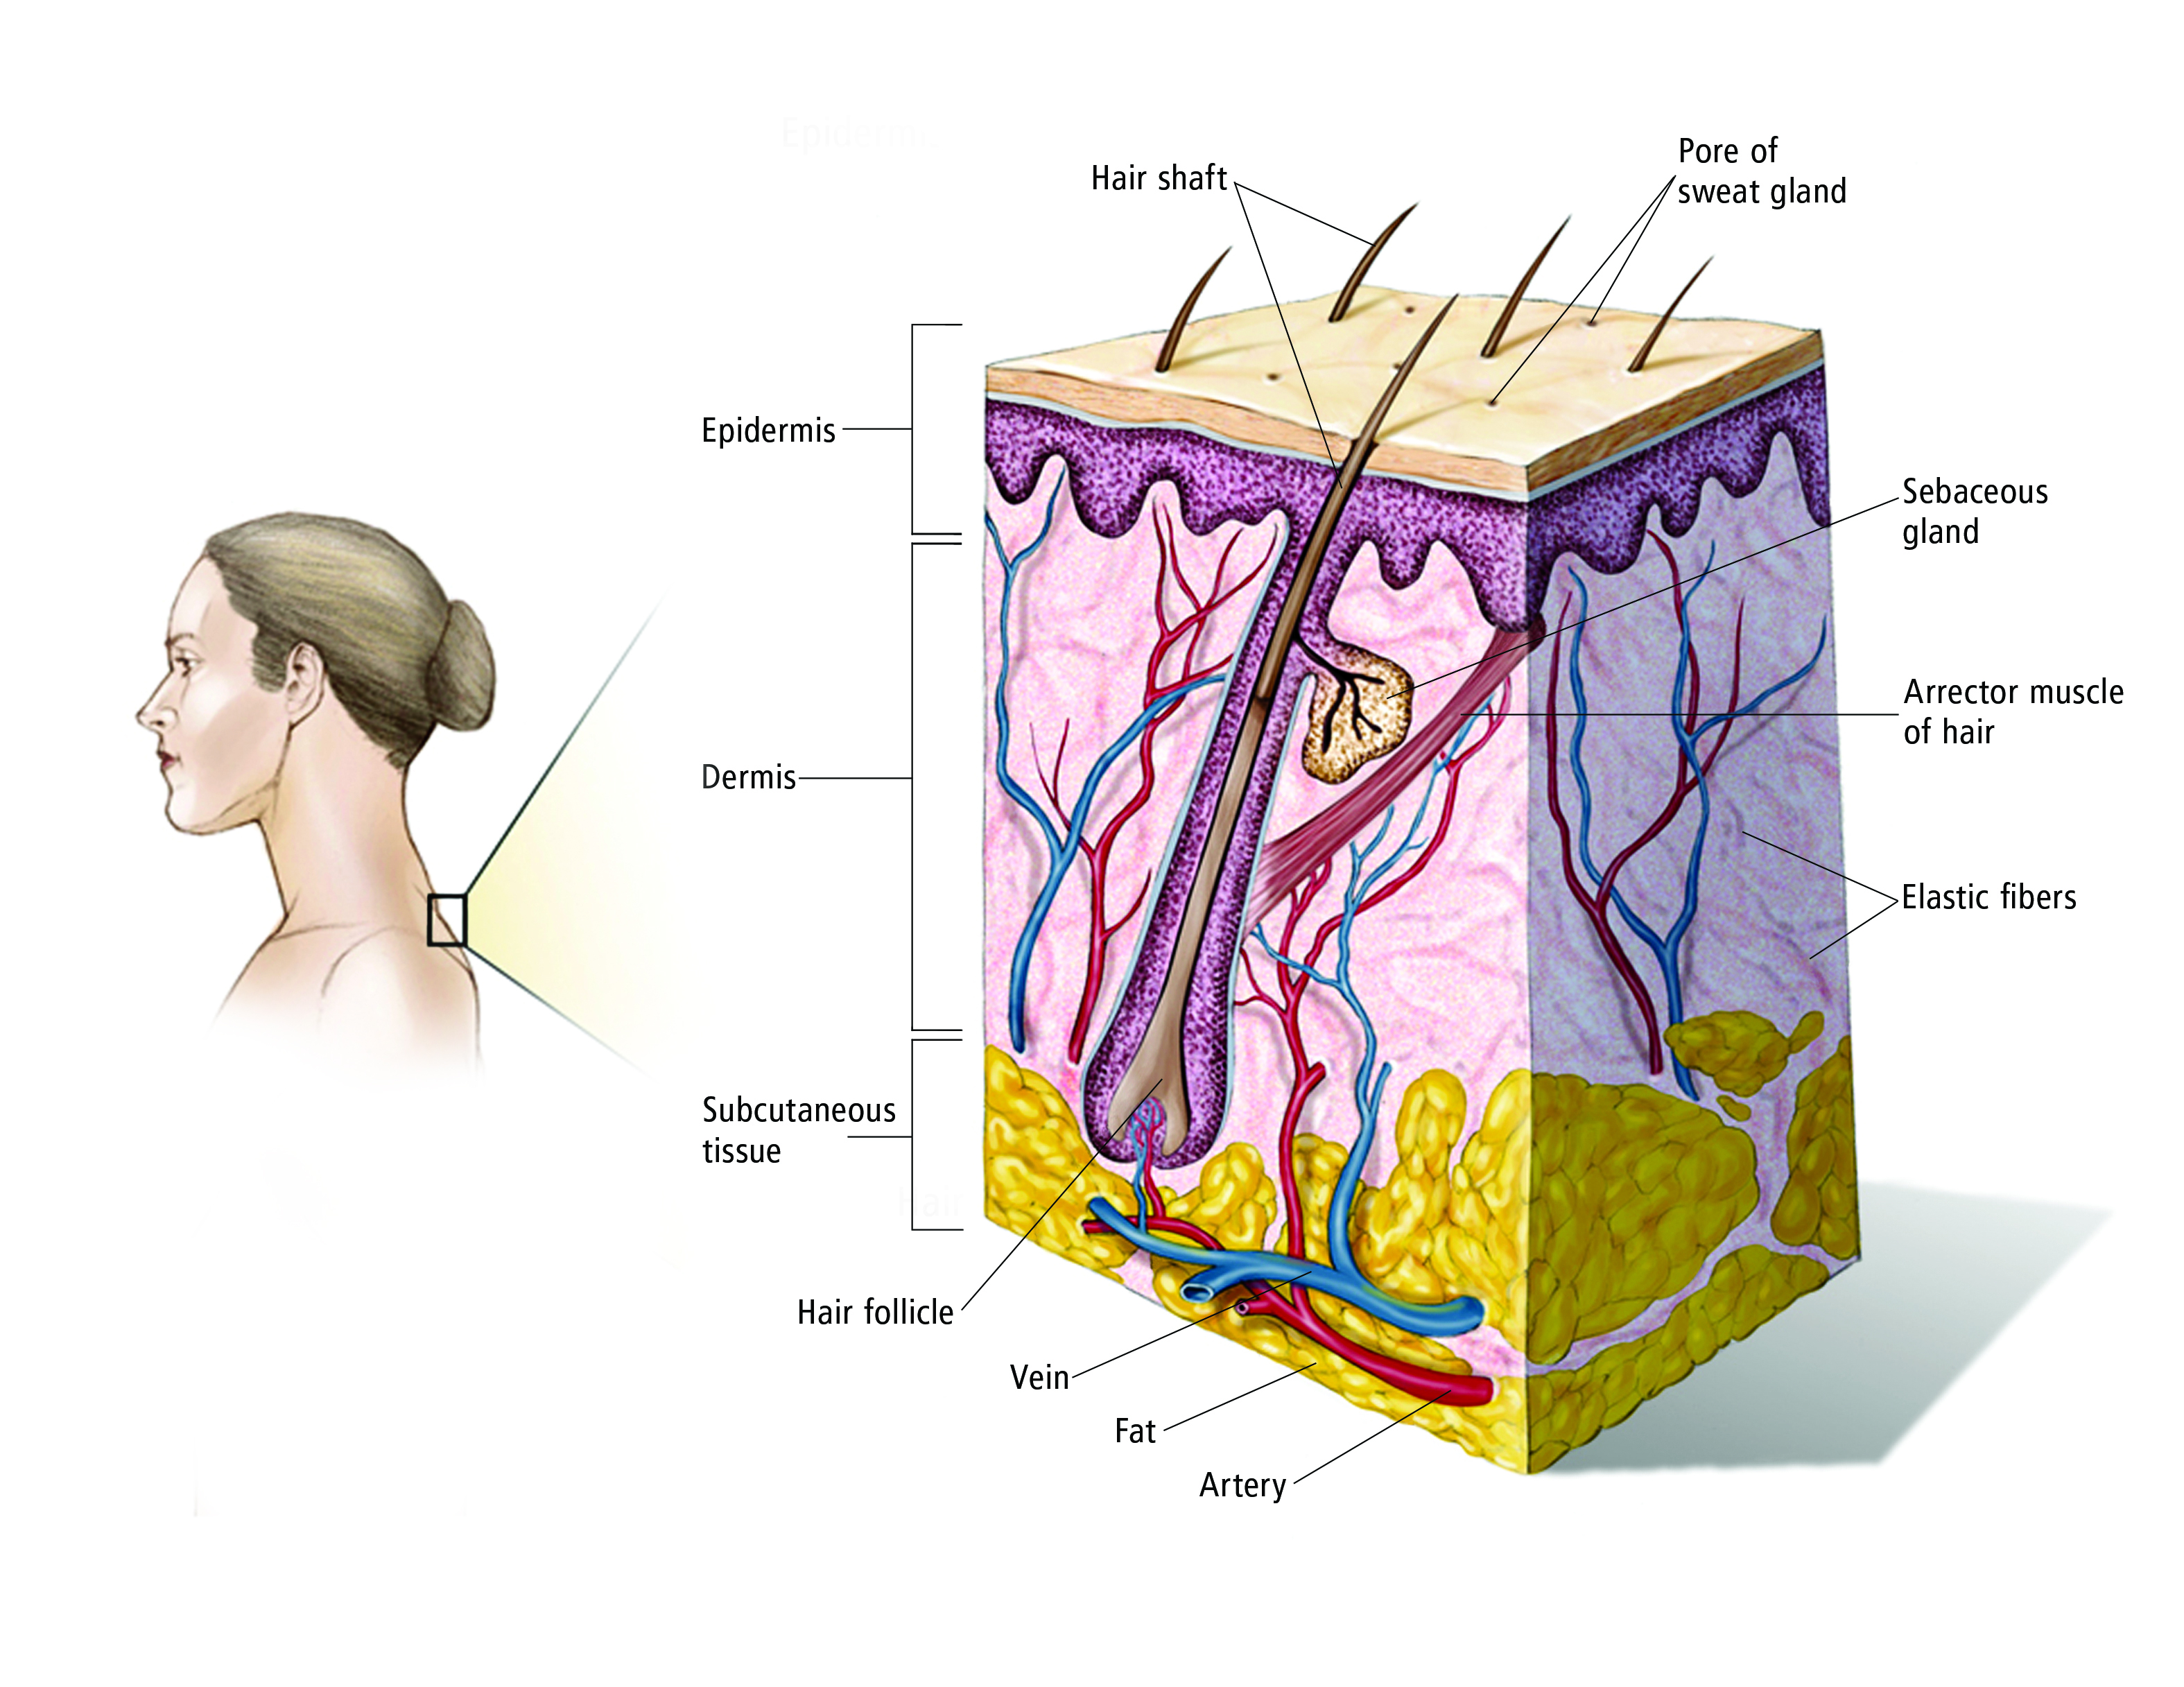
\includegraphics[width=0.85\textwidth]{imatges/problem_domain/melanoma-diagram.jpg}
  \caption[Skin Main Layers]{\textit{Skin Main Layers. Illustration by
Cancer.Net}} {\label{fig:melanoma_diagram}} \end{figure}

\section{Skin Cancer}

Cancer begins when healthy cells undergo changes that cause them to grow and
divide uncontrollably, forming a mass known as a tumor. Tumors can be
classified as either cancerous or benign. A cancerous tumor is considered
malignant, meaning it has the potential to invade nearby tissues and spread to
other parts of the body through a process called metastasis. Conversely, a
benign tumor may grow locally but does not have the ability to spread to other
areas. \\

Skin cancer is one of the most prevalent types of cancer, with over 3 million
Americans diagnosed each year. However, the prognosis for skin cancer is
generally favorable when detected early. Treatment options for skin cancer
often involve topical medications, in-office procedures performed by
dermatologists, or outpatient surgeries. Dermatologists specialize in
diagnosing and treating conditions of the skin. As a result, skin cancer
accounts for less than 1\% of all cancer-related deaths. \\

In more advanced cases, skin cancer may require comprehensive medical care
provided by a multidisciplinary team, which typically includes a dermatologist,
surgical oncologist, radiation oncologist, and clinical oncologist.

\subsection{Types of Skin Cancer}

There are three primary forms of skin cancer \cite{BaseCancerKnowledge}.

\begin{itemize}

  \item \textbf{Basal cell carcinoma}

    This type of skin cancer arises from basal cells located in the lower
    epidermis. Approximately 80\% to 90\% of skin cancers originate from
    these cells, leading to the designation of basal cell carcinomas. They
    typically develop on the head and neck, although they can occur anywhere
    on the skin. Sun exposure is the primary cause, although they may also
    occur in individuals who underwent radiation therapy during childhood.
    This type of skin cancer generally grows slowly and rarely metastasizes
    to other parts of the body.

  \item \textbf{Squamous cell carcinoma}

    This type of skin cancer originates from flat, scale-like cells known as
    squamous cells that comprise a significant portion of the epidermis.
    Around 10\% to 20\% of skin cancers develop from these cells, resulting
    in the classification of squamous cell carcinomas. Sun exposure is the
    main cause, and they can be diagnosed on various regions of the skin.
    They may also emerge on skin that has been burned, damaged by chemicals,
    or exposed to x-rays. Common sites for squamous cell carcinoma include
    the lips, areas with long-standing scars, and the skin surrounding the
    mouth, anus, and vagina. Roughly 2\% to 5\% of squamous cell carcinomas
    metastasize to other parts of the body.

  \item \textbf{Melanoma}

    The most aggressive type of skin cancer, originates in scattered cells
    known as melanocytes where the epidermis and dermis meet. Melanocytes
    produce the pigment melanin, responsible for skin color. Melanoma
    accounts for approximately 1\% of all skin cancers.

\end{itemize}

\subsection{Stages of Skin Cancer}

The following stages are used for basal cell carcinoma. Basal cell carcinoma
accounts for more than 90\% of all skin cancers in the United States and is the
most common of all cancers. Typically, it is a slow-growing cancer that seldom
spreads to other parts of the body \cite{CancerInstitute}. \\

\begin{itemize}

  \item \textbf{Stage I}

    In stage I, abnormal cells are found in the squamous cell or basal cell
    layer of the epidermis. These abnormal cells may become cancer and spread
    into nearby normal tissue.

    \begin{figure}[H] \centering
      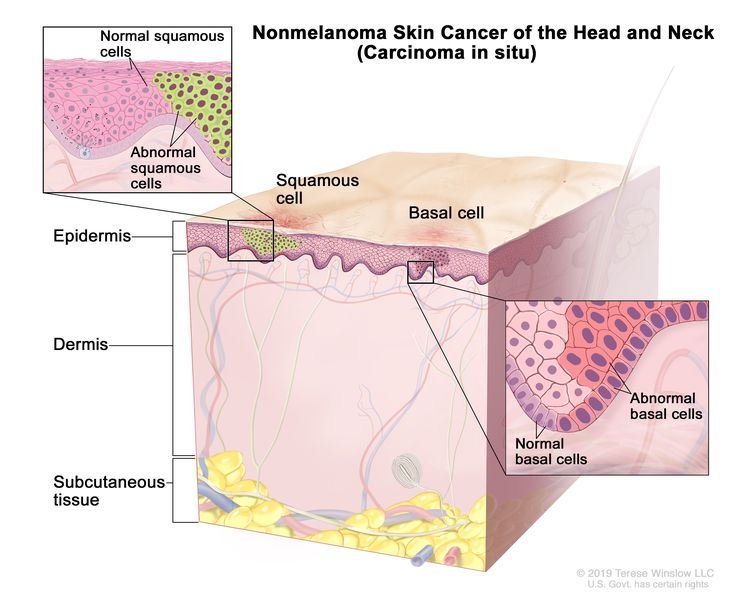
\includegraphics[width=0.6\textwidth]{imatges/problem_domain/phase0-skin-cancer.jpg}
      \caption[Skin Cancer, Stage I]{\textit{Skin Cancer, Stage I. Illustration by Terese Winslow}}
    {\label{fig:stage0-skin-canceer}} \end{figure}

    \newpage


  \item \textbf{Stage II}

    In stage II, cancer has formed and the tumor is 2 centimeters or smaller.

    \begin{figure}[H] \centering
      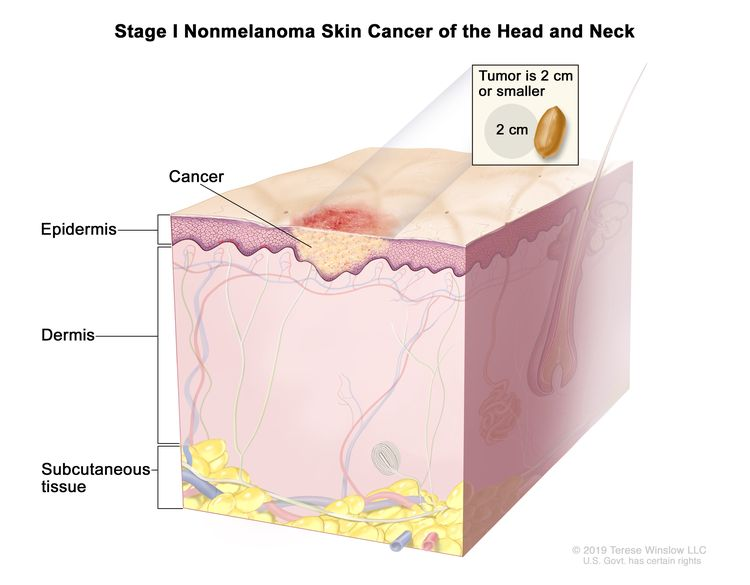
\includegraphics[width=0.6\textwidth]{imatges/problem_domain/stage1-skin-cancer.jpg}
      \caption[Skin Cancer, Stage II]{\textit{Skin Cancer, Stage II.
      Illustration by Terese Winslow}} {\label{fig:stage1-skin-canceer}}
    \end{figure}


  \item \textbf{Stage III}

    In stage II, the tumor is larger than 2 centimeters but not larger than 4
    centimeters.

    \begin{figure}[H] \centering
      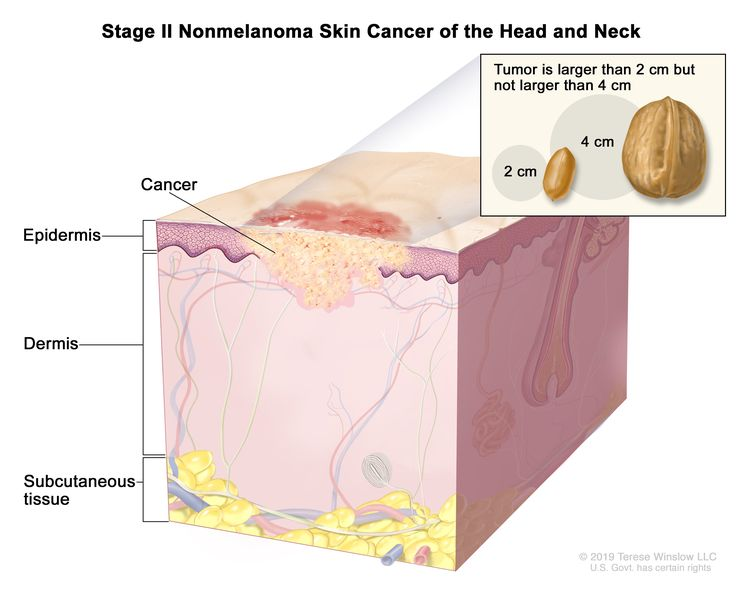
\includegraphics[width=0.6\textwidth]{imatges/problem_domain/stage2-skin-cancer.jpg}
      \caption[Skin Cancer, Stage III]{\textit{Skin Cancer, Stage III.
      Illustration by Terese Winslow}} {\label{fig:stage2-skin-canceer}}
    \end{figure}

    \newpage

  \item \textbf{Stage IV}

    In this stage, the cancer may spread to the rest of the body covering the
    nerves bellow the dermis or bellow the subcutaneous tissue or the bones.

    \begin{figure}[H] \centering
      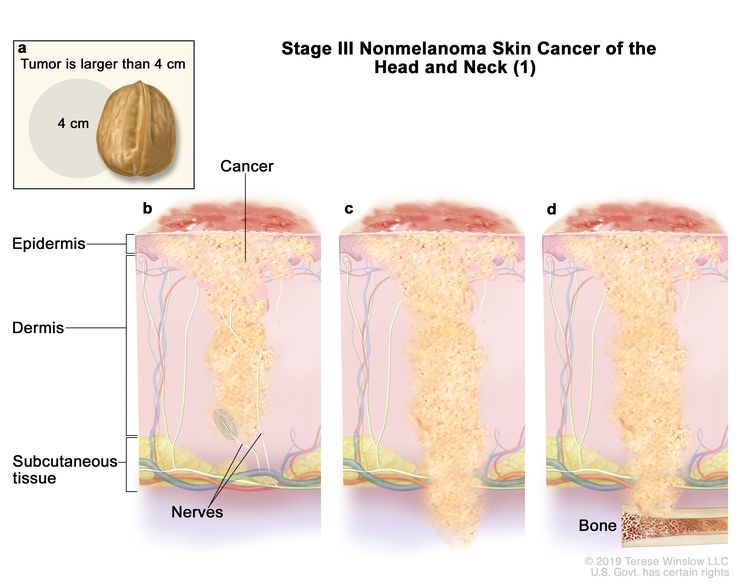
\includegraphics[width=0.6\textwidth]{imatges/problem_domain/stage3-skin-cancer.jpg}
      \caption[Skin Cancer, Stage IV]{\textit{Skin Cancer, Stage IV. Illustration by
    Terese Winslow}} {\label{fig:stage3-skin-canceer}} \end{figure}

\end{itemize}

\subsection{Associated Factors and Prevention of Skin Cancer}

The risk factors associated with skin cancer encompass sun exposure, fair skin,
as well as certain physical characteristics such as blond hair and blue eyes.
The presence of melanin, a protein responsible for the skin's color or pigment,
plays a crucial role in shielding the skin from ultraviolet (UV) radiation.
Consequently, individuals with lighter skin or lower levels of melanin possess
reduced UV protection \cite{OrigenAndTreatment}. \\

Although skin cancer may initially appear to predominantly affect individuals
with light complexions, those with dark skin are also susceptible. They may
observe signs of cancer on the palms of their hands or soles of their feet.
\\

Advancements in research have led to treatments targeting the genetic level.
New drug therapies assist in stimulating the immune system to produce
antibodies capable of combatting rapidly dividing cells. While these therapies
may have potential side effects, they are generally milder than those
associated with chemotherapy. Moreover, they result in an enhanced immune
system that is better equipped to battle cancer. \\

A patient's overall health also appears to influence their ability to fight
cancer, although the precise connection between one's health and their risk of
developing cancer remains unclear. However, it can be assumed that better
overall health enhances the immune system's capacity to combat cancer. \\

Prevention of skin cancer is straightforward: minimizing exposure to the sun
and UV radiation. Ceasing the use of tanning beds is advised. When exposed to
the sun, wearing sunscreen and a wide-brimmed hat that provides comprehensive
head shading is recommended \cite{OrigenAndTreatment}. \\

Consideration should also be given to wearing clothing with SPF protection.
Some clothing manufacturers now produce summer attire with SPF levels similar
to those found in sunscreen. This is significant since most regular t-shirts
offer only minimal SPF protection of around 2. \\

Skin cancer ranks among the most prevalent forms of cancer, yet it is also one
of the most easily detectable and treatable. Taking proactive measures to
prevent sun exposure is crucial, while early detection is highly important. The
prognosis is favorable when melanoma is identified in its early stages.


\chapter{Preliminaries}
\label{cap:prelim}

The objective of this chapter is to provide a comprehensive overview that defines the scope of the thesis.
It covers essential theoretical and technical concepts necessary to comprehend the experiments presented in subsequent chapters.

\section{Artificial Intelligence}

\textit{AI} is one of the newest fields in science and engineering. Work started in earnest soon
after World War II, and the name itself was coined in 1956 attributed by John McCarthy of MIT. \\

After successfully decrypting Enigma\footnote{Enigma was a rotor machine designed to encrypt and decrypt messages.}, in World War II, the mathematician Alan Turing posed a groundbreaking question that had a profound impact on society: "Can machines think?" \cite{CanMachineThink}. In this seminal work, Turing not only outlined the process of developing intelligent machines but also presented a method for assessing their intelligence. Even today, the Turing Test remains a widely recognized benchmark for evaluating the intelligence of artificial systems. According to this test, if a human cannot distinguish, through a text-based conversation, whether they are interacting with a human or a machine, the artificial system can be considered to possess intelligence. \\

The term "AI" is exciting but, the definition of this term is blurry \cite{AIModernApprouch}.
Historically there are two approaches to \textit{AI} that have been followed, each by different people
with different methods. The human-centered approach and the rationalist approach. The incorporation of a human-centered approach into the field must incorporate empirical scientific methods, which entail making observations and formulating hypotheses about human behavior. On the other hand, a rationalist approach combines the disciplines of mathematics and engineering. These different perspectives have both faced criticism and received praises. \\

From that juncture until the turn of the century, the field of \textit{AI} encountered fluctuations, witnessing periods of remarkable accomplishments interspersed with the infamous \textit{AI} winters. Currently \textit{AI} is a hot topic of discussion, evident from the increasing searches and online mentions. While \textit{AI} has been around for more than 65 years, the recent exponential trend can be attributed to the availability of cost-efficient storage, transfer, and computation capabilities for massive amounts of data. This newfound capacity was previously unimaginable and has contributed to the current \textit{AI} boom. \\

\textit{AI} has expanded into numerous distinct fields, showcasing its extensive range of applications, techniques, and interdisciplinary nature. The diversity of branches in the field of artificial intelligence is represented in \textit{Figure \ref{fig:ai_branches}}, which depicts several current \textit{AI} fields. However, it is important to note that the figure can be further expanded to include additional fields, such as Speech Processing and Expert Systems, among others.

\begin{figure}[H]
\centering
\resizebox{0.8\textwidth}{!}{%
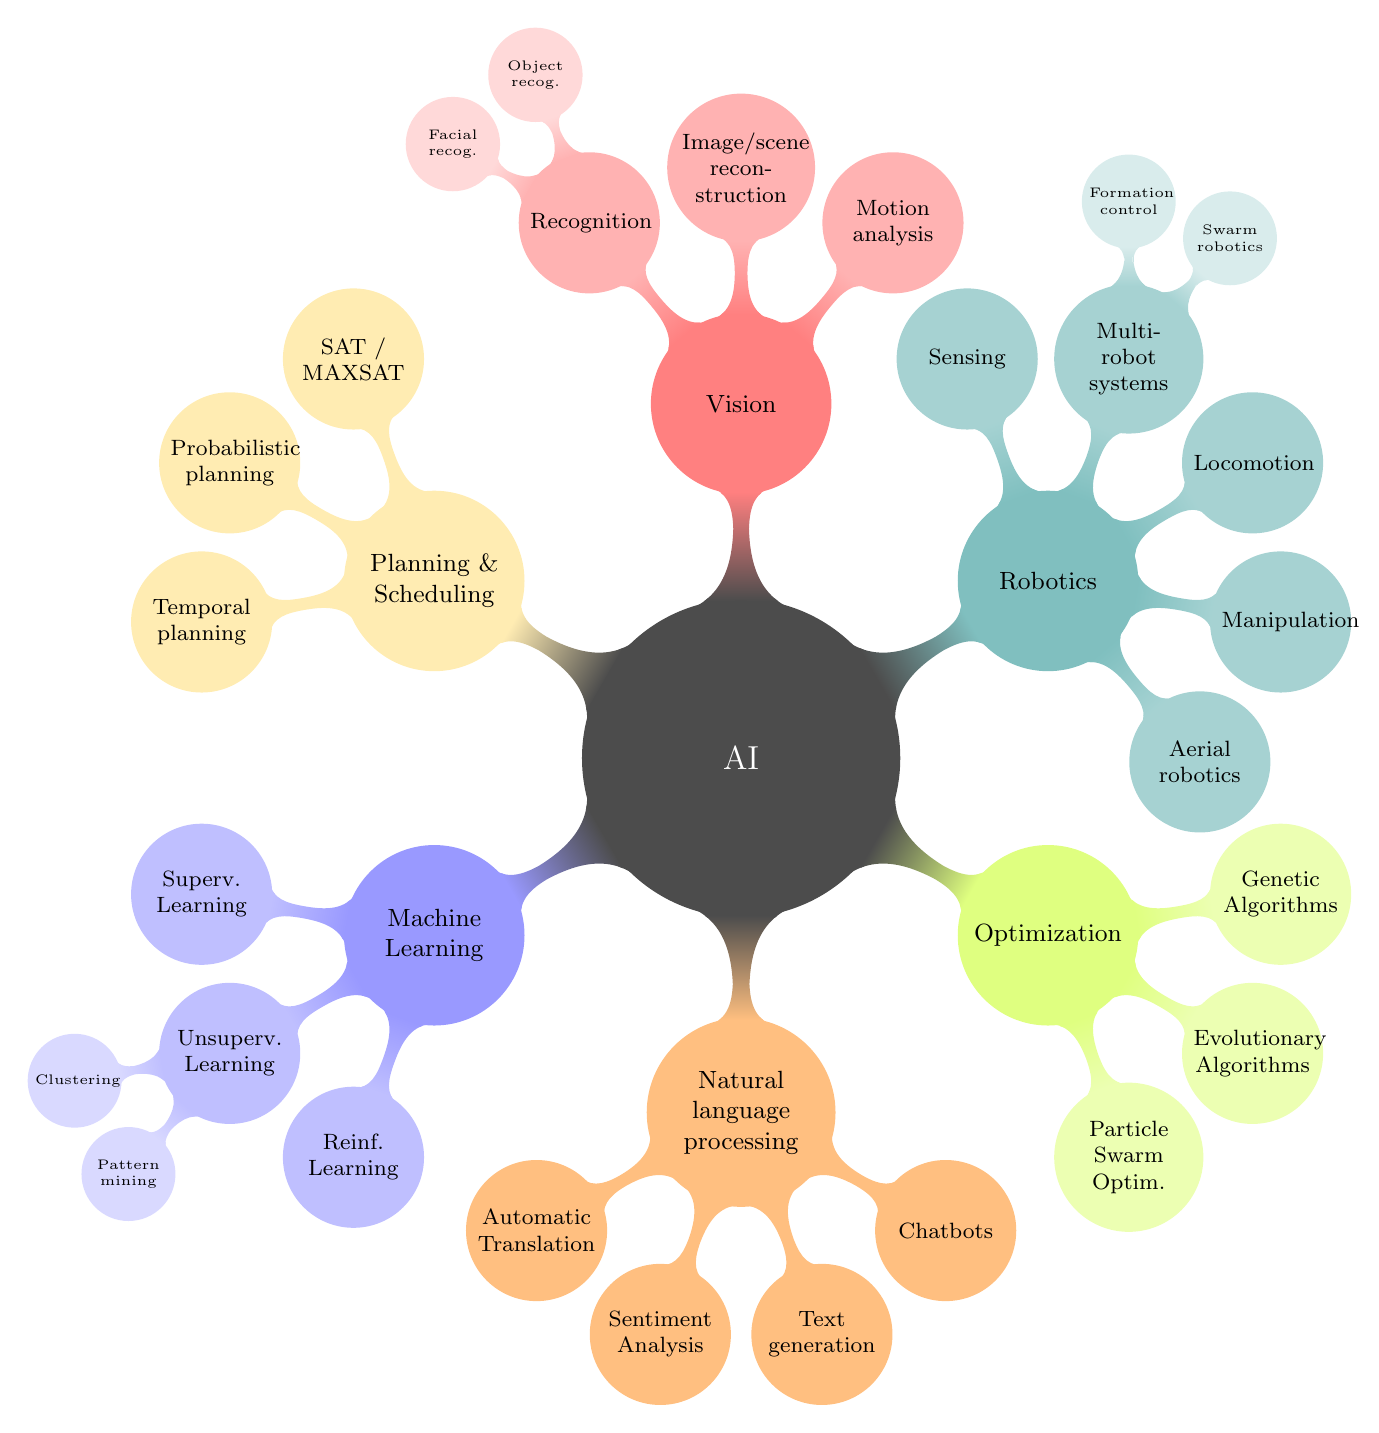
\begin{tikzpicture}[mindmap, grow cyclic, every node/.style=concept, concept color=black!70, text = white,
    level 1/.append style={level distance=4.5cm,sibling angle=60},
    level 2/.append style={level distance=3cm,sibling angle=40},
    level 3/.append style={level distance=2cm,sibling angle=40}]

\node{AI}
    child [concept color=blue!40, text = black] { node {Machine Learning}
        child [concept color=blue!25]{ node {Superv. Learning}}
        child [concept color=blue!25]{ node {Unsuperv. Learning}
            child [concept color=blue!15]{ node {Clustering}}
            child [concept color=blue!15]{ node {Pattern mining}}
        }
        child [concept color=blue!25]{ node {Reinf. Learning}}
    }
    child [concept color=orange!50, text = black] { node {Natural language processing}
        child { node {Automatic Translation}}
        child { node {Sentiment Analysis}}
        child { node {Text generation}}
        child { node {Chatbots}}
    }
    child [concept color=lime!50, text = black] { node {Optimization}
        child [concept color=lime!30]{ node {Particle Swarm Optim.}}
        child [concept color=lime!30]{ node {Evolutionary Algorithms}}
        child [concept color=lime!30]{ node {Genetic Algorithms}}
    }
    child [concept color=teal!50, text = black] { node {Robotics}
        child [concept color=teal!35]{ node {Aerial robotics}}
        child [concept color=teal!35]{ node {Manipulation}}
        child [concept color=teal!35]{ node {Locomotion}}
        child [concept color=teal!35]{ node {Multi-robot systems}
            child [concept color=teal!15]{ node {Swarm robotics}}
            child [concept color=teal!15]{ node {Formation control}}
        }
        child [concept color=teal!35]{ node {Sensing}}
    }
    child [concept color=red!50, text = black] { node {Vision}
        child [concept color=red!30]{ node {Motion analysis}}
        child [concept color=red!30]{ node {Image/scene reconstruction}}
        child [concept color=red!30]{ node {Recognition}
            child [concept color=red!15]{ node {Object recog.}}
            child [concept color=red!15]{ node {Facial recog.}}
        }
    }
    child [concept color=amber!30, text = black] { node {Planning \& Scheduling}
        child { node {SAT / MAXSAT}}
        child { node {Probabilistic planning}}
        child { node {Temporal planning}}
    };
\end{tikzpicture}%
}
\caption[AI Sub-Specialists]{\textit{\textit{AI} Sub-Specialists. Note that these subfields often intersect and combine. Illustration by Author}}
{\label{fig:ai_branches}}
\end{figure}

\newpage

\section{Machine Learning}

Machine learning is a branch of artificial intelligence (\textit{AI}) and computer science which focuses on the use of data and algorithms to imitate the way that humans learn, gradually improving its accuracy \cite{IBMMachineLearning}. The term \textit{AI} was defined by the pioneer Arthur Samuel as “the field of study that gives computers the ability to learn without explicitly being programmed.” \\

The central idea of machine learning is the existence of a mathematical relationship between any combination of input and output data. Rather than manually programming knowledge into computers, machine learning endeavors to automatically learn significant relationships and patterns by observing examples. \\

There are three subcategories (\textit{Figure \ref{fig:ml_branches}}) of machine learning \cite{MITML}. These subcategories are listed bellow. \\

\begin{itemize}
\item \textbf{Supervised Learning}

Machine learning models are trained with labeled data sets, which allow the models to learn and grow more accurate over time. For example, an algorithm would be trained with pictures of dogs and other things, all labeled by humans, and the machine would learn ways to identify pictures of dogs on its own. Supervised machine learning is the most common type used today. \\

\item \textbf{Unsupervised Learning}

Unsupervised learning involves using a training set that comprises unlabeled inputs, meaning inputs that do not have any assigned desired output. The primary objective of this learning approach is to uncover concealed patterns or data clusters without relying on human intervention. \\

\item \textbf{Reinforcement Learning}

Reinforcement learning occupies a position between supervised and unsupervised learning. In a certain sense, there is some form of supervision, but it does not involve explicitly specifying a desired output for every input in the data. Instead, a reinforcement learning algorithm receives feedback from the environment only after selecting an output, known as an action, based on a given input or observation. The feedback indicates the extent to which the action fulfills the learner's goals. \\

\end{itemize}

\begin{figure}[H]
\centering
\resizebox{0.65\textwidth}{!}{%
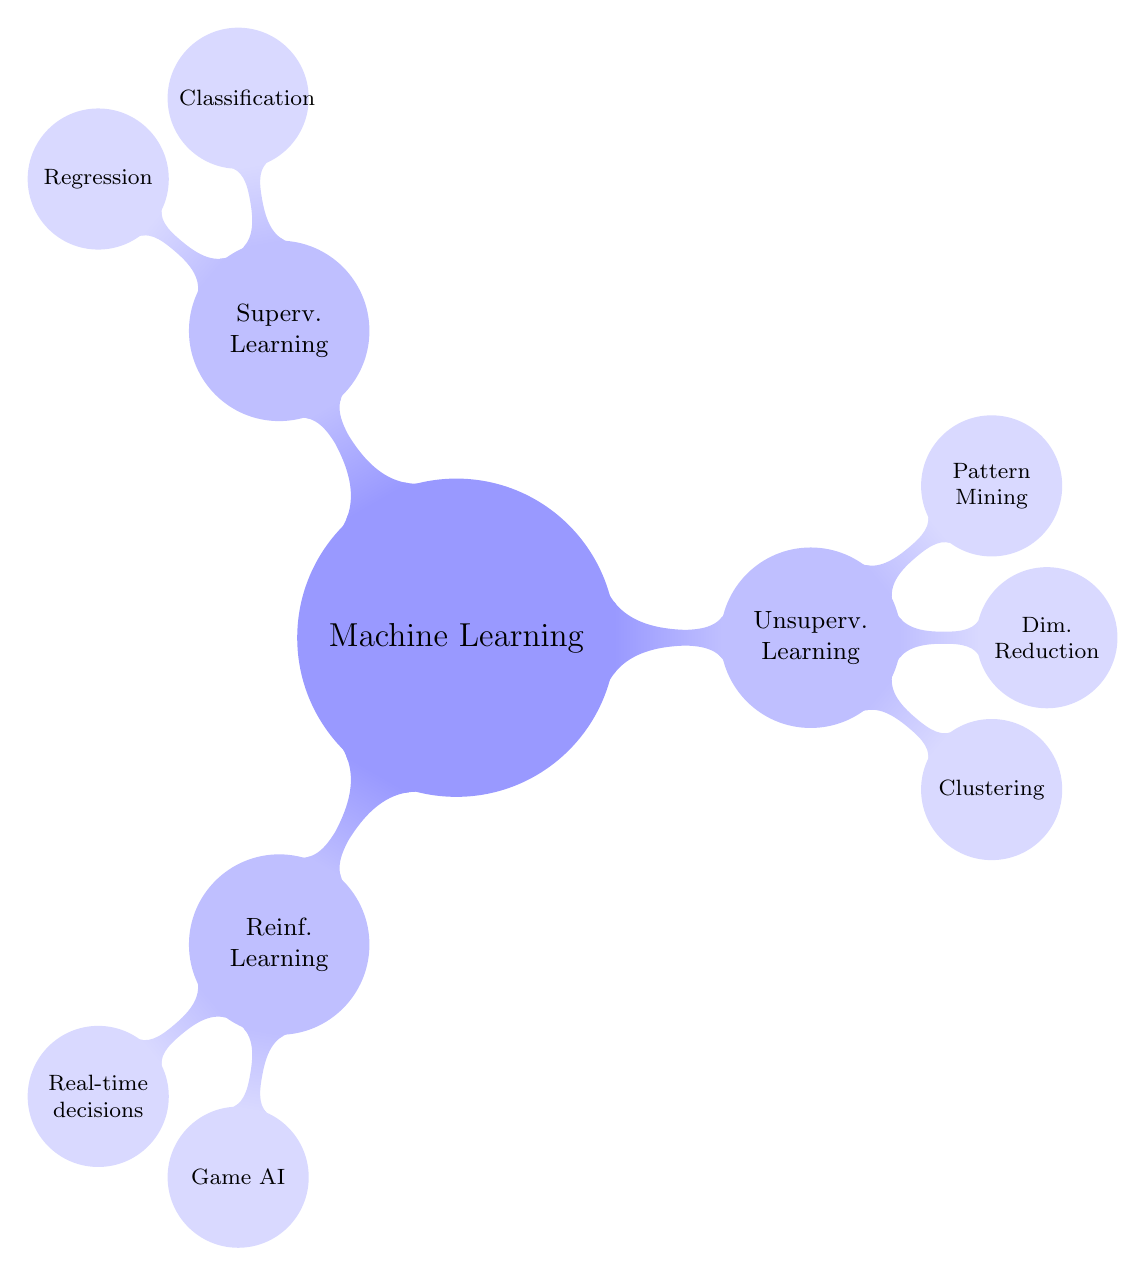
\begin{tikzpicture}[mindmap, grow cyclic, every node/.style=concept, concept color=blue!40, text = black,
    level 1/.append style={level distance=4.5cm,sibling angle=120},
    level 2/.append style={level distance=3cm,sibling angle=40},
    level 3/.append style={level distance=2cm,sibling angle=40}]

\node{Machine Learning}
    child [concept color=blue!25, text = black] { node {Reinf. Learning}
        child [concept color=blue!15]{ node {Real-time decisions}}
        child [concept color=blue!15]{ node {Game AI}}
    }
    child [concept color=blue!25, text = black] { node {Unsuperv. Learning}
        child [concept color=blue!15]{ node {Clustering}}
        child [concept color=blue!15]{ node {Dim. Reduction}}
        child [concept color=blue!15]{ node {Pattern Mining}}
    }
    child [concept color=blue!25, text = black] { node {Superv. Learning}
        child [concept color=blue!15]{ node {Classification}}
        child [concept color=blue!15]{ node {Regression}}
    };
\end{tikzpicture}%
}
\caption[Subcategories of Machine Learning.]{\textit{Subcategories of Machine Learning. Illustration by Author}}
{\label{fig:ml_branches}}
\end{figure}


\section{Deep Learning}

Deep learning, is a subset of machine learning algorithms, is primarily associated with supervised learning techniques. This algorithms derive conclusions by analyzing data with a given logical structure. In contrast to traditional machine learning algorithms, deep learning algorithms operate at a higher level of abstraction. They possess the ability to perform the laborious process of feature extraction. Each algorithm applies a nonlinear transformation to its input and uses the acquired knowledge to generate a statistical model as the output. This iterative process continues until the output reaches an acceptable level of accuracy. The term "deep" refers to the number of layers the data must pass through during these iterations. \\

Deep learning has been successfully applied to various problems, ranging from self-driving cars to speech recognition. In this particular project, deep learning is employed to classify whether a given dermoscopy image is a melanoma or not. To achieve this, it has been necessary to understand how convolutional neural networks work, address certain issues that affect the precision of these models, explain the key metrics primarily used to measure the accuracy of these models.


\section{Deep Neural Networks}

Deep neural networks are part of the deep learning algorithms within the realm of machine learning, which, as mentioned earlier, falls under the umbrella of artificial intelligence. \textit{Figure \ref{fig:deep-learning-family}} is an illustration of the deep learning family. \\

\begin{figure}[H]
\centering
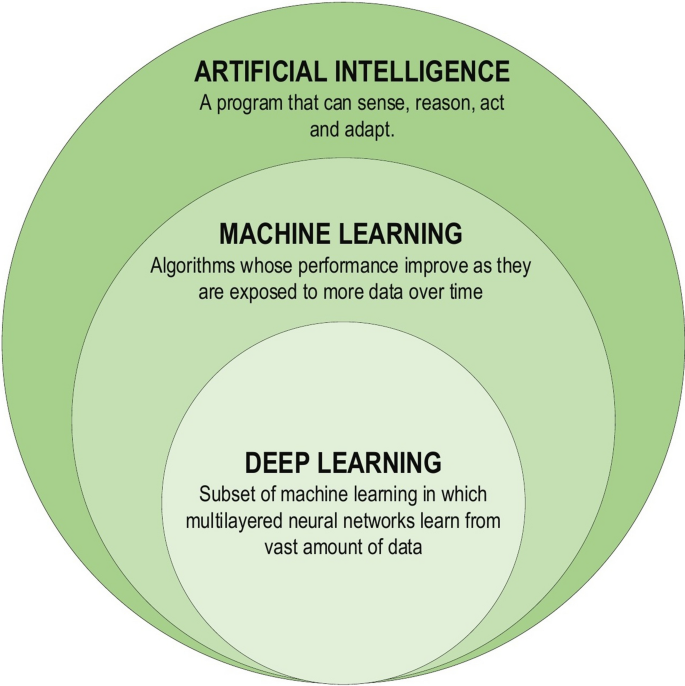
\includegraphics[width=0.6\textwidth]{imatges/preliminaries/deep-learning-familiy.png}
\caption[Deep Learning Family]{\textit{Deep Learning Family. Illustration by towardsdatascience}}
{\label{fig:deep-learning-family}}
\end{figure}

Deep neural networks, also known as fully connected layers, are modeled after the human brain. These algorithms achieve their functionality by propagating signals from the input layer to the output layer while passing through intermediate hidden layers. Each layer consists of neurons responsible for detecting patterns from the incoming connections. These neurons perform a crucial task by combining input from the data with a corresponding set of coefficients, also known as weights. These weights act as amplifiers or dampeners, modulating the impact of the input on the neuron's activation. \\

By leveraging this mechanism, each layer in the deep neural network acquires the capability to capture distinctive features from the input data. Notably, as the signal travels deeper into the network, the extracted features become increasingly sophisticated and abstract. This characteristic arises from the hierarchical nature of the network architecture, enabling the model to learn and discern intricate patterns and representations. \\

The process of feature extraction in deep neural networks allows the network to progressively learn and uncover complex relationships within the data. As the signal traverses through the network's layers, each subsequent layer builds upon the extracted features from the previous layer, resulting in the generation of more intricate and comprehensive representations. This ability to capture and model hierarchical features is a significant advantage of deep neural networks, making them particularly effective in tasks requiring the recognition of complex patterns and high-level abstractions.

\begin{figure}[H]
\centering
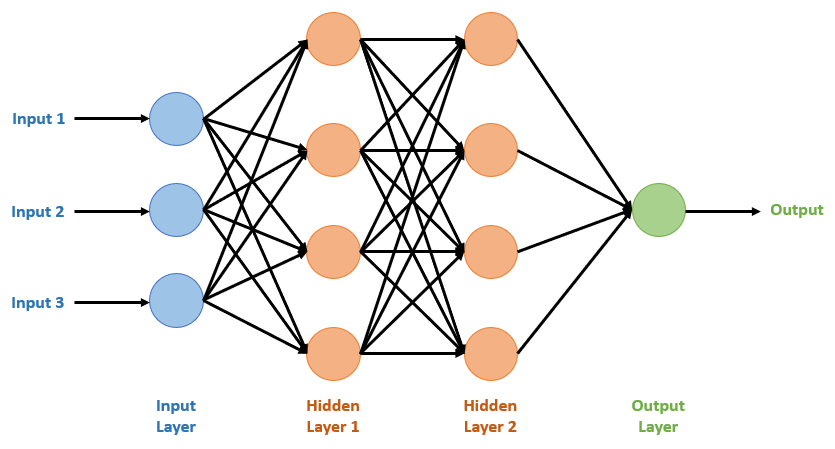
\includegraphics[width=0.8\textwidth]{imatges/preliminaries/deep-neural-network.png}
\caption[Deep Neural Network]{\textit{Deep Neural Network. This NN has two hidden layers. Illustration by Introduction to Neural Networks in Deep Learning}}
{\label{fig:deep-nn}}
\end{figure}

The minimum unit in a layer is known as neuron or perceptron (\textit{Figure \ref{fig:perceptron}}).
The perceptron, is the oldest simple neural network, created by Frank Rosenblatt in 1958.
Every node within the network possesses an associated value, which is computed based on the incoming nodes and edges. The computation takes place in the following manner: the products
of  inputs and their respective weights are summed with a bias, and this sum is subsequently passed through the node's activation function.
The activation function serves the purpose of compressing the resulting value within the range of 0 to 1 and introduces non-linearity,
allowing the model to learn complex relationships in the data. The resulting value determines the
degree to which the signal should propagate through the network, ultimately influencing the final outcome.

\begin{figure}[H]
\centering
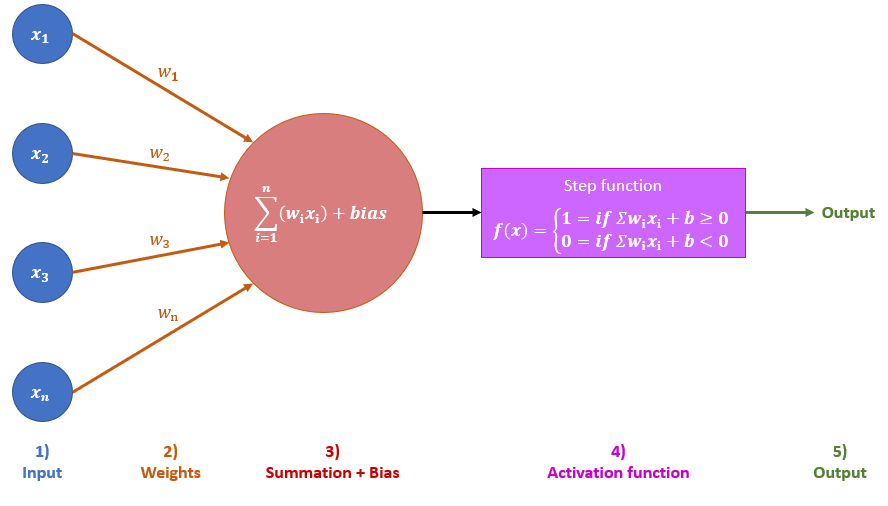
\includegraphics[width=0.75\textwidth]{imatges/preliminaries/perceptron.png}
\caption[The Perceptron]{\textit{The Perceptron. Illustration by Introduction to Neural Networks in Deep Learning}}
{\label{fig:perceptron}}
\end{figure}


\section{Convolutional Neural Networks}

A convolutional neural network (CNN) is a specific type of neural network that is particularly well-suited for analyzing visual imagery. It draws inspiration from the organization of the animal visual cortex, which is responsible for visual processing in living organisms. \\

One of the key innovations of CNNs is their ability to automatically learn a large number of filters in parallel. These filters are learned during the training process and are specifically tailored to solve a particular predictive modeling problem, such as image classification. By learning these filters, CNNs become adept at extracting relevant features and patterns from visual data without the need for manual feature engineering. \\

CNNs are designed to learn spatial hierarchies of features through a process called back-propagation. During training, the network adapts its internal parameters, or weights, by iteratively propagating the error backwards from the output to the input layers. This allows the network to gradually adjust its weights in a way that minimizes the difference between its predicted outputs and the true outputs. \\

One key distinction of CNNs compared to regular neural networks is their use of parameter sharing. In a CNN, all neurons within a particular feature map share the same weights. This sharing of weights significantly reduces the number of parameters in the network, making it more computationally efficient. By sharing weights, the network can detect the same patterns or features regardless of their spatial position in the input data. This property, known as translation invariance, enables CNNs to recognize objects or patterns regardless of their location within an image.\\

Furthermore, CNNs have a three-dimensional arrangement of neurons: width, height, and depth. The width and height dimensions correspond to the spatial dimensions of the input data, such as the width and height of an image. The depth dimension refers to the number of channels or feature maps in each layer, where each channel represents a different aspect or feature of the input. \\

To build CNN architectures, there are four main types of layers.

\subsection{Convolutional Layers}

A convolutional layer (\textit{Figure \ref{fig:convolutional-layer}}) is responsible for detecting and extracting features from the input data. It consists of a set of learnable filters, also known as kernels or feature detectors. Each filter is a small matrix of weights that slides or convolves across the input data to perform a dot product operation at each spatial location.  \\

The filter slides or convolves across the input data with a defined stride, which specifies the amount of shift between each position.
At each spatial location, a dot product is computed between the filter and the overlapping region of the input.
The dot product involves element-wise multiplication of the filter values with the corresponding input values, followed by summing up the results. \\

The result of each dot product operation is a single value, forming a pixel in the output feature map. Additionally, an activation function is applied element-wise to introduce non-linearity into the network. \\

\newpage

\begin{figure}[H]
\centering
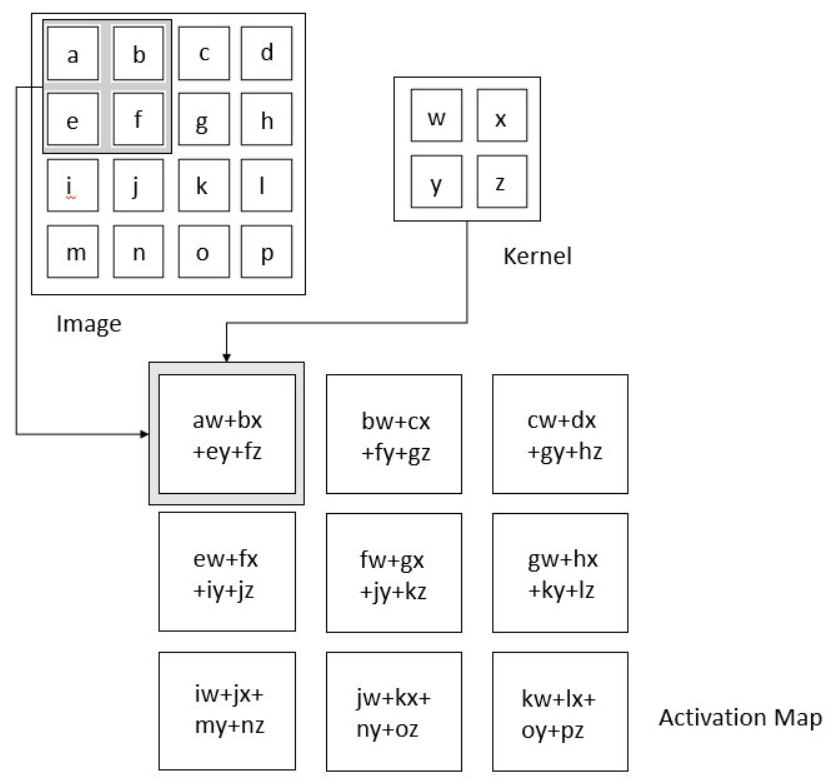
\includegraphics[width=0.8\textwidth]{imatges/preliminaries/convolutional-layer.png}
\caption[Convolutional Operation on Input Image]{\textit{Convolutional Operation on Input Image. Illustration by towardsdatascience}}
{\label{fig:convolutional-layer}}
\end{figure}


\subsection{Pooling Layers}

A pooling layer (\textit{Figure \ref{fig:pooling-layer}}) performs a summarizing of nearby outputs in the network, effectively replacing certain locations with a condensed representation. This reduces the spatial dimensionality of the output, leading to decreased computational requirements and weight parameters. The pooling operation is applied independently to each slice of the representation. \\

Various pooling functions exist, including averaging the values within a rectangular neighborhood, computing the L2 norm of the neighborhood, or using a weighted average based on distance. However, the most widely used method is max pooling, which selects the maximum output value from the neighborhood.

\newpage

\begin{figure}[H]
\centering
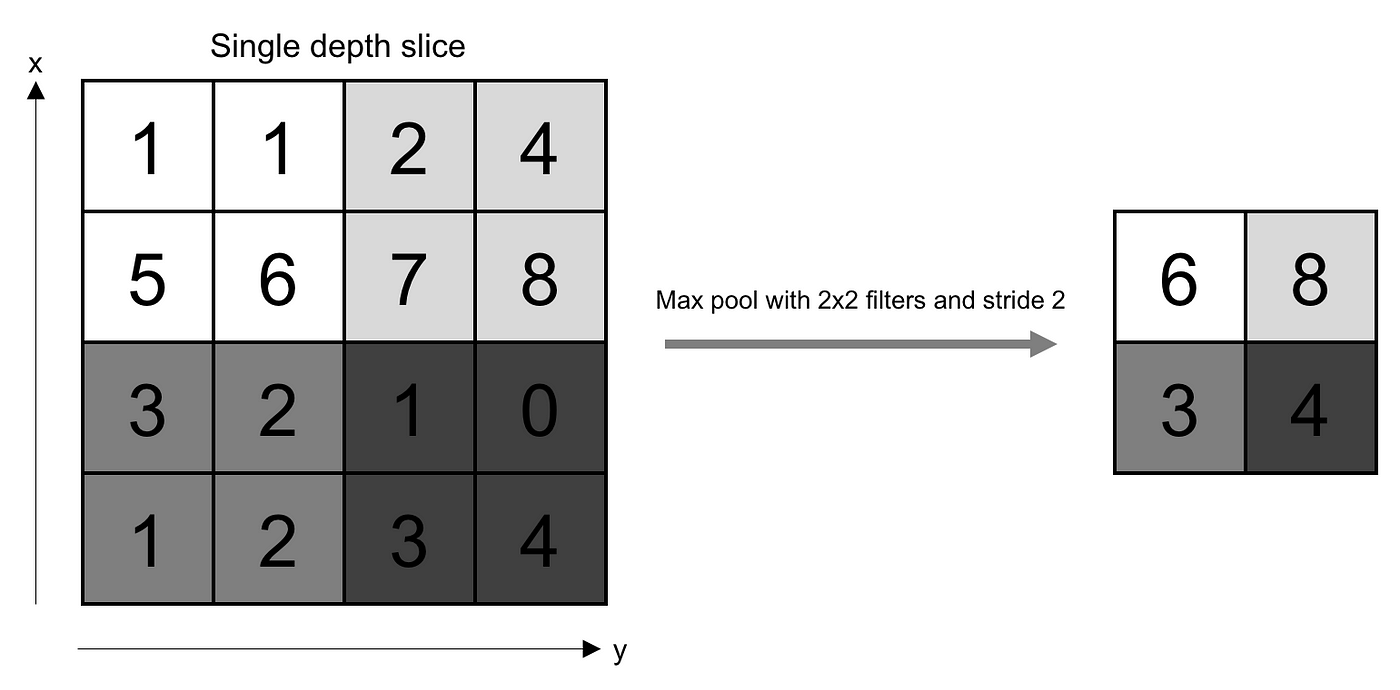
\includegraphics[width=0.8\textwidth]{imatges/preliminaries/polling-layer.png}
\caption[Max Polling Operation on Input Image]{\textit{Max Polling Operation on Input Image. Illustration by towardsdatascience}}
{\label{fig:pooling-layer}}
\end{figure}

\subsection{Fully Connected Layers}

Neurons in this layer have full connectivity with all neurons in the preceding and succeeding layer. This is why it can be computed as usual by a matrix multiplication followed by a bias effect. The topology in the fully connected portion of a CNN depends on various factors, including the complexity of the task, the nature of the data, and the capacity of the model. There is no fixed rule for determining the exact number of neurons or layers, and it often requires experimentation and tuning. \\

The fully connected layer helps to map the representation between the input and the output. See \textit{Figure \ref{fig:deep-nn}} to a visual representation of a fully connected layer. \\

\subsection{Non-linearity Layers}

Convolutional operations in neural networks are linear, meaning they capture linear patterns in the data. However, many objects in images exhibit non-linear characteristics that cannot be effectively detected using linear operations alone. To address this limitation, non-linearity layers, such as activation functions, are typically applied immediately after the convolutional layer. These non-linearity layers introduce non-linear transformations to the activation maps, enabling the network to learn and detect complex, non-linear patterns in the data. \\

There are many types of non-linearity functions applied after the convolutional layers, the most popular are: \\

\begin{itemize}

\item \textbf{Sigmoid}

The sigmoid function takes a real-valued number and “squashes” it into a range between 0 and 1.

\centering {
\begin{tikzpicture}
  \draw[->] (-5,0) -- (5,0) node[right] {$x$};
  \draw[->] (0,-0.5) -- (0,1.5) node[above] {$\sigma(x)$};
  \draw[domain=-5:5, smooth, variable=\x, blue] plot (\x, {1/(1 + exp(-\x))});
  \draw[dashed] (-5, 0.0) node[left] {0};
  \draw[dashed] (-5, 1) node[left] {1} -- (5, 1);
\end{tikzpicture}
}

\raggedright
Mathematically, the sigmoid function is expressed as:

\[ \sigma(x) = \frac{1}{1 + e^{-x}} \]

\item \textbf{ReLU}

The Rectified Linear Unit (ReLU) is maybe the most popular activation functions in the last few years. The function is just simply threshold at zero.

\centering
\begin{tikzpicture}
  \draw[->] (-5,0) -- (5,0) node[right] {$x$};
  \draw[->] (0,-0.5) -- (0,5) node[above] {$\text{ReLU}(x)$};
  \draw[domain=-5:0, smooth, variable=\x, blue] plot (\x, 0);
  \draw[domain=0:5, smooth, variable=\x, blue] plot (\x, \x);
  \draw[dashed] (-5, 0.0) node[left] {0};
    \draw[dashed] (-5, 1) node[left] {1} -- (5, 1);
\end{tikzpicture}

\raggedright
Mathematically, the ReLU function is expressed as:

\[f(x) = \max(0, x)\]

\item \textbf{Tanh}

The hyperbolic tangent function tanh compresses a real-valued number to the range of [-1, 1]. Similar to the sigmoid function, tanh exhibits saturation, but unlike sigmoid, its output is centered around zero.

\centering
\begin{tikzpicture}
  \draw[->] (-5,0) -- (5,0) node[right] {$x$};
  \draw[->] (0,-1.5) -- (0,1.5) node[above] {$\tanh(x)$};
  \draw[domain=-5:5, smooth, variable=\x, blue] plot (\x, {tanh(\x)});
  \draw[dashed] (-5, -1) node[left] {-1} -- (5, -1);
  \draw[dashed] (-5, 1) node[left] {1} -- (5, 1);
\end{tikzpicture}

\raggedright
Mathematically, the tanh function is expressed as:

\[ \tanh(x) = \frac{{e^x - e^{-x}}}{{e^x + e^{-x}}} \]

\end{itemize}

\section{Loss Function}

A loss function, also known as a cost function or an objective function, is a measure used in machine learning and optimization algorithms to quantify how well a model performs on a given task. It represents the discrepancy between the predicted outputs of a model and the true values or labels associated with the training data. \\

Different machine learning tasks and algorithms may use different loss functions, depending on the specific problem being addressed. Commonly used loss functions include:

\begin{itemize}
    \item Mean Squared Error (MSE)
    \item Binary Cross-Entropy
    \item Mean Absolute Error (MAE)
    \item Cross-entropy Loss
\end{itemize}

For this thesis, the loss function used to train the models is
{\tt Cross-entropy Loss} as this is a multiclass problem. Don't confuse the optimizer
algorithm with the metric used to evaluate how good models are.
We used the ROC AUC with one-vs-rest strategy to evaluate the models performance, explained in \textit{Section \ref{sec:metrics}}. \\

Cross-entropy loss, also known as log loss, is a widely used loss function in machine learning, particularly in classification tasks. It measures the dissimilarity between predicted class probabilities and true class labels. \\

In multi-class classification, the cross-entropy loss is calculated using the true class labels \(y\) and the predicted class probabilities \(p\) for each class. It can be defined as:

\[-\sum_{i=1}^{C} y_i \log(p_i)\]

\noindent where:

\begin{itemize}
    \item \(C\) is the total number of classes.
    \item \(y_i\) represents the true label for class \(i\).
    \item \(p_i\) represents the predicted probability for class \(i\).
\end{itemize}

\section{Metrics}
{\label{sec:metrics}}

There are various metrics commonly used to assess the quality of a model's predictions.
In this section, we present a selection of metrics that we find relevant for evaluating our models.

\subsection{Confusion Matrix}

A confusion matrix (\textit{Figure \ref{fig:confusion-matrix}}) is a square matrix with dimensions {\tt NxN},
where {\tt N} represents the total number of classes being predicted.
It provides a visual representation of the errors or confusion made by a classification
model during its predictions. \\

From confusion matrix we can obtain other metrics such as:

\begin{itemize}
\item \textbf{True Positive (TP)}

This refers to an outcome where the model accurately predicts the positive class.
\item \textbf{False Positive (FP)}

This describes a situation where the model mistakenly predicts the positive class when it should have predicted the negative class.
\item \textbf{True Negative (TN)}

This represents an outcome where the model correctly predicts the negative class.
\item \textbf{False Negative (FN)}

This indicates a scenario where the model incorrectly predicts the negative class instead of predicting the positive class.

\end{itemize}

\begin{figure}[H]
\begin{adjustbox}{trim={0pt 0.5cm 0pt 1cm}, clip}
\centering
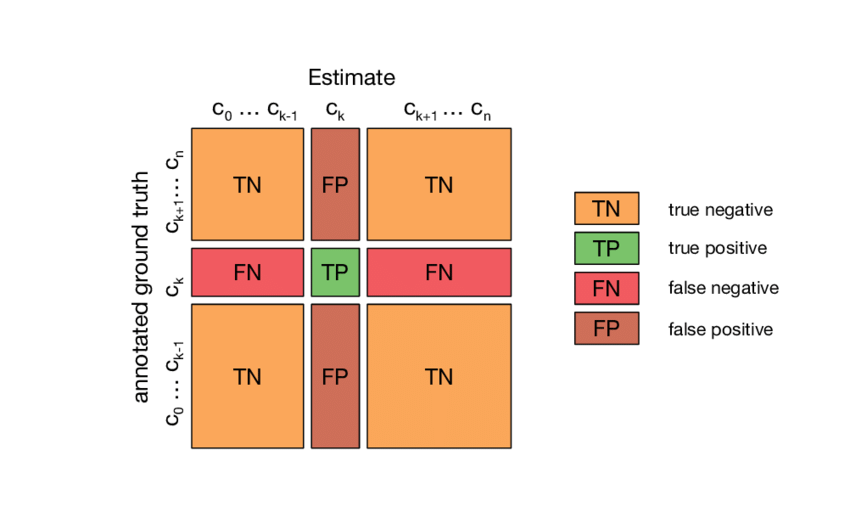
\includegraphics[width=0.9\textwidth]{imatges/preliminaries/confusion-matrix.png}
\end{adjustbox}
\caption[Confusion Matrix Multi-Class]{\textit{Confusion Matrix Multi-Class. Illustration by kaggle}}
{\label{fig:confusion-matrix}}
\end{figure}

In a logical sense, when we add up the elements on the main diagonal of the confusion matrix,
we obtain the total number of correct predictions.
Conversely, summing the elements on the antidiagonal provides us with the total number of incorrect predictions.
Utilizing these values, we can compute additional metrics such as accuracy, precision, recall, specificity, and F1 score.

\subsection{Accuracy}

Accuracy is a commonly employed and straightforward performance metric in classification tasks. It calculates the ratio of correct predictions to the total number of predictions made on a dataset, thus determining the likelihood of correctly classifying an input. Accuracy is especially valuable when working with a balanced dataset, where the number of instances in each class is roughly equivalent. However, in the case of the previously mentioned thesis dataset, which is not balanced, the use of accuracy serves primarily to monitor model training performance rather than being the main evaluation metric.

\[Accuracy = \frac{TP + TN}{TP + TN + FP + FN}\]

\subsection{TPR}

TPR stands for True Positive Rate, and it is also known as sensitivity or recall.
It measures the proportion of actual positive cases that are correctly identified as positive
by a classification model or test.

\[
\text{TPR} = \frac{\text{TP}}{\text{TP} + \text{FN}}
\]

\item \textbf{FPR}

FPR stands for False Positive Rate, and it measures the proportion of actual negative cases that are incorrectly identified as positive by a classification model or test.

\[
\text{FPR} = \frac{\text{FP}}{\text{FP} + \text{TN}}
\]

\subsection{AUC-ROC Curve with One-vs-Rest Strategy}

The ROC Curve, when computed with the one-vs-rest (OvR) strategy for multiclass classification, provides insights into how well the model can differentiate a class from the rest of the classes. It is a probabilistic curve that plots the true positive rate (TPR) against the false positive rate (FPR). By treating the target class as the positive class and the remaining classes as the negative class in separate binary classification tasks (\textit{Figure \ref{fig:auc-roc}}). \\

The area under the curve (AUC) is a value between 0 and 1 that measures
the ability of a classifier to distinguish between classes. It is used as a summary
of the ROC curve. The higher the AUC, the better the performance of the
model at distinguishing between the positive and negative classes.

\begin{figure}[H]
\centering
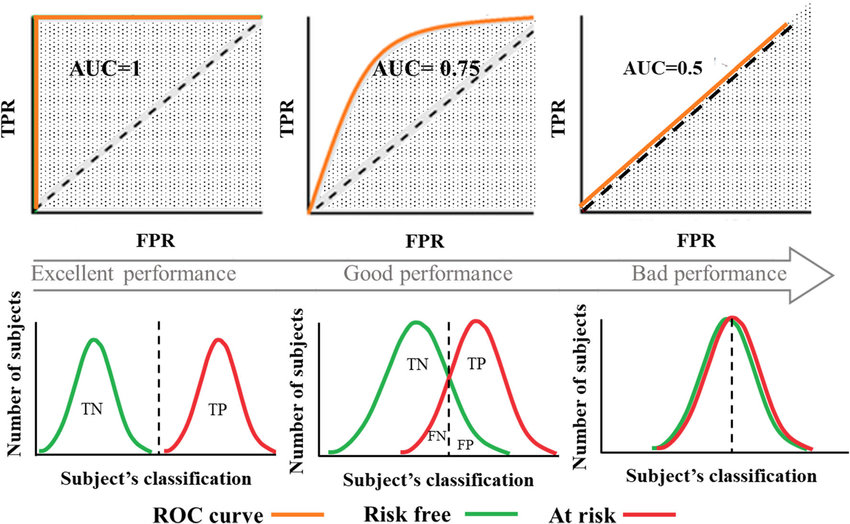
\includegraphics[width=0.8\textwidth]{imatges/preliminaries/auc.png}
    \caption[Forward Propagation and Backward Propagation]{\textit{AUC-ROC. Comparison of multiple ROC curves and how much overlap there are between classes. Illustration by Elizabeth Louise Thomas}}
{\label{fig:auc-roc}}
\end{figure}


\section{Optimizer}

An optimizer is an algorithm that finds the value of the parameters (weights) that minimize the error when mapping inputs to outputs. These optimization algorithms widely affect the accuracy and speed training of the deep learning models. \\

While training a deep learning models, the optimizer modifies the weights of the model in each epoch to minimize the loss function. \\

The are a considerable amount of different optimizer algorithms out there with their pros and cons.
In this section I present the family of optimizers based on Gradient Descent optimization. This family of optimizer algorithms were used for the thesis. \\

\subsection{Gradient Descent}

Using the Gradient Decent optimization algorithm, the weights are updated incrementally after each epoch (pass over the training dataset). \\

The magnitude and direction of the weight update is computed by taking a step in the opposite direction of the cost gradient.

\[\nabla J(w) = (\frac{\partial J}{\partial w_1}, \frac{\partial J}{\partial w_2}, \ldots, \frac{\partial J}{\partial w_n})\]

\[
\Delta w = -\eta \cdot \nabla J(w)
\]

Finally, the weight are updated after each epoch with the following expression:

\[
w = w + \Delta w
\]


\begin{itemize}
    \item \(\Delta w\) represents the weight update.
    \item \(\eta\) (eta) denotes the learning rate, which controls the step size of the update.
    \item  \(\frac{\partial J}{\partial w_i}\) represents the partial derivative of the cost function \(J\) with respect to the weight \(w_i\).
    \item \(\nabla J(w)\) represents the gradient of the cost function \(J(w)\) with respect to the weights \(w\).
\end{itemize}

In Gradient Descent optimization, we compute the cost gradient based on the complete training set; hence, we sometimes also call it batch gradient descent. In case of very large datasets, using Gradient Descent can be quite costly since we are only taking a single step for one pass over the training set – thus, the larger the training set, the slower our algorithm updates the weights and the longer it may take until it converges to the global cost minimum. \\

A high level pseudo-implementation of the Gradient Descent algorithm:

\begin{itemize}[label=\(\circ\)]
  \item for each epoch:
  \begin{itemize}[label=\(\circ\), topsep=0pt]
    \item for each weight \(j\):
    \begin{itemize}[label=\(\circ\), topsep=5pt]
      \item \(w_j = w_{j-1} + \Delta w_j\)
    \end{itemize}
  \end{itemize}
\end{itemize}

The \textit{Figure \ref{fig:optimization}} shows how the Gradient Descent optimizer would try to modify the  the weight values that minimizes the cost function.

\begin{figure}[H]
\centering
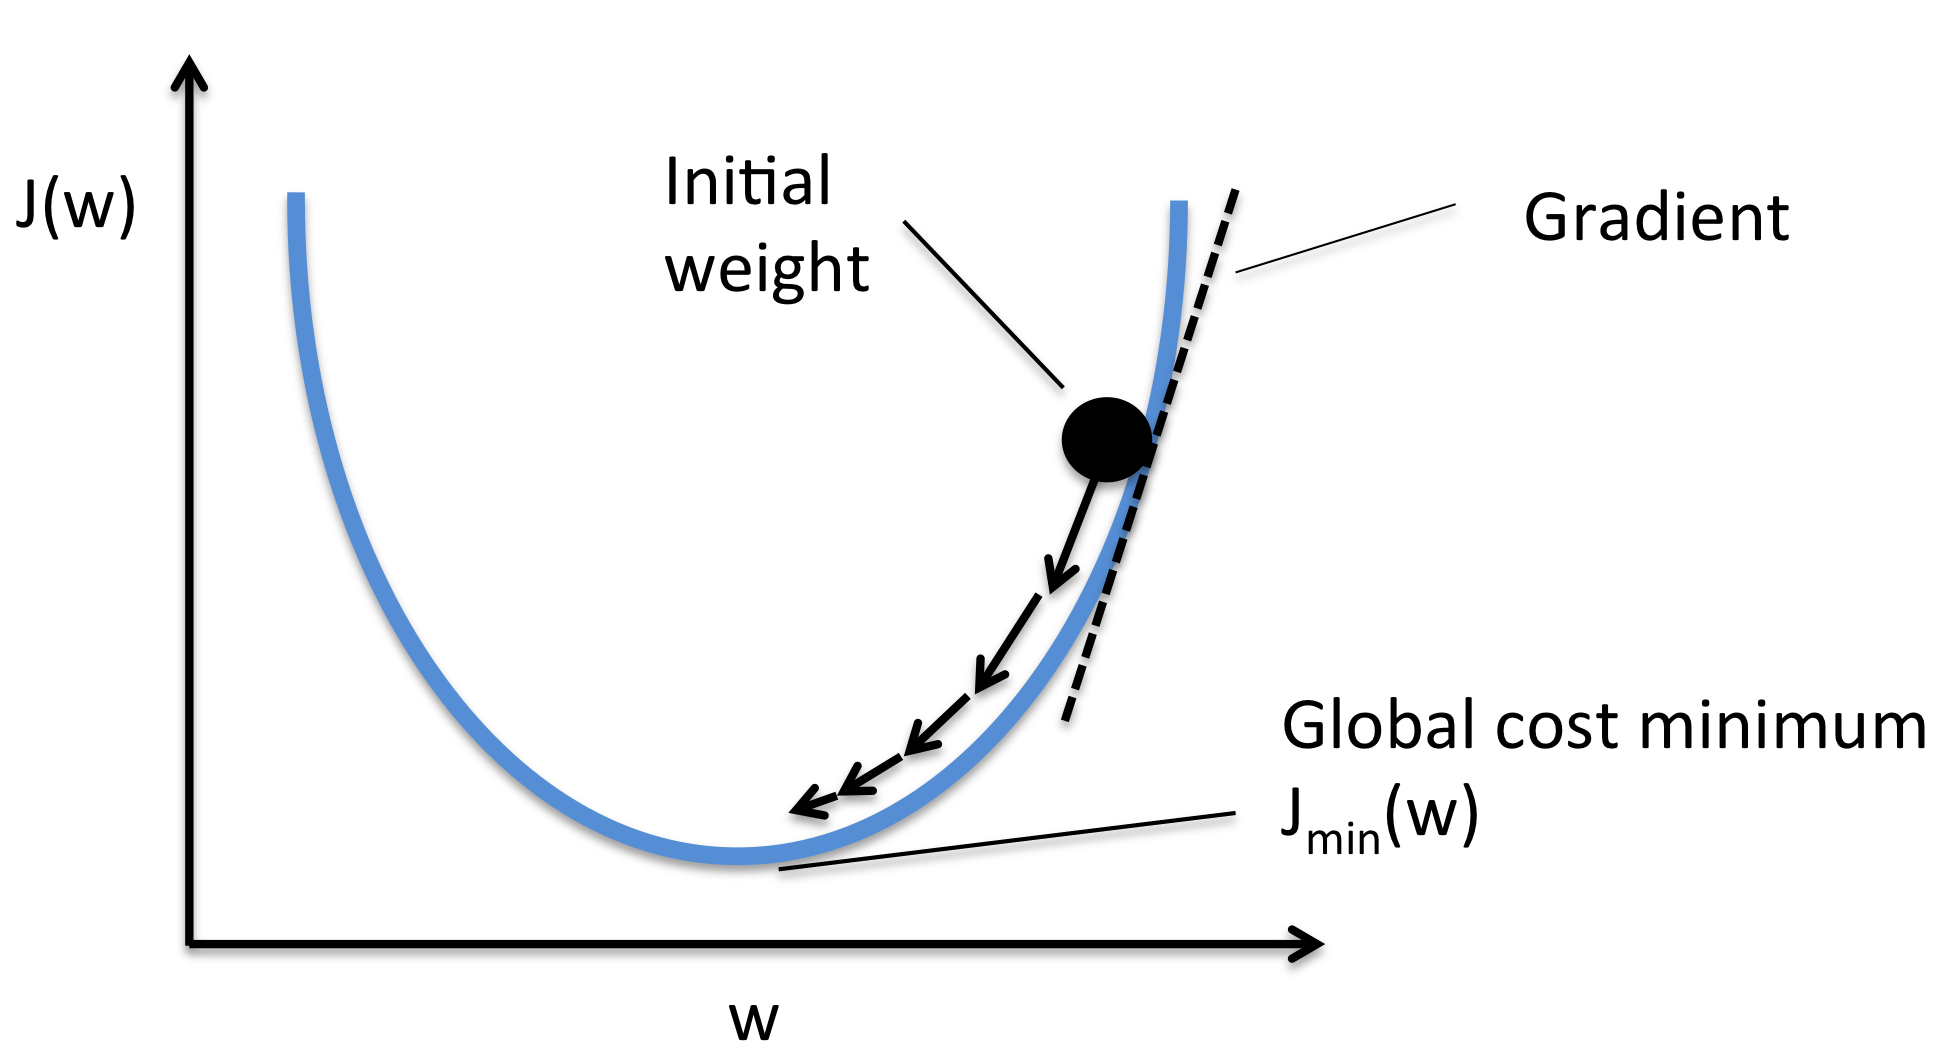
\includegraphics[width=0.7\textwidth]{imatges/preliminaries/optimization.png}
    \caption[Function Optimization]{\textit{Function Optimization. Optimization of a 2D function using Gradient Descent algorithm. Illustration by sebastianraschka}}
{\label{fig:optimization}}
\end{figure}

\newpage

\subsection{Stochastic Gradient Descent}

Stochastic Gradient Descent work similar to the Gradient Descent but the weight updates are not accumulated as we’ve seen above for Gradient Descent. Instead, the weights are updated after each training sample. Due to its stochastic nature, the path towards the global cost minimum is not “direct” as in Gradient Descent, but may go “zig-zag”if we are visuallizing the cost surface in a 2D space, see \textit{Figure \ref{fig:sgdvsgd}}. However, it has been shown that Stochastic Gradient Descent almost surely converges to the global cost minimum if the cost function is convex. \\

A high level pseudo-implementation of the Stochastic Gradient Descent algorithm:

\begin{itemize}[label=$\circ$]
    \item for each epoch or until approx. cost minimum is reached:
        \begin{itemize}[label=$\circ$, topsep=0pt]
            \item for training sample \(i\):
              \begin{itemize}[label=$\circ$, topsep=5pt]
                \item for each weight \(j\):
                    \begin{itemize}[label=$\circ$, topsep=10pt]
                        \item \(w_j = w_{j-1} + \Delta w_j\), where \(\Delta w_j = \eta (target^{(i)} - output^{(i)})x_{j}^{(i)}\)
                    \end{itemize}
            \end{itemize}
        \end{itemize}
\end{itemize}

\begin{figure}[H]
\centering
\begin{adjustbox}{trim=0cm 0cm 0cm 1cm, clip}
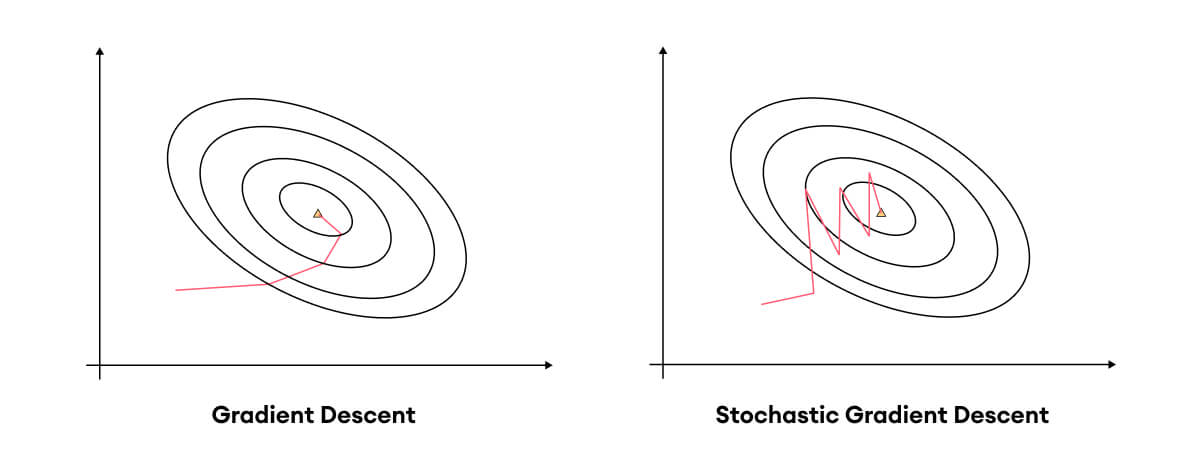
\includegraphics[width=0.9\textwidth]{imatges/preliminaries/sgdvsgd.jpeg}
\end{adjustbox}
    \caption[Gradient Descent vs Stochastic Gradient Descent]{\textit{Gradient Descent vs Stochastic Gradient Descent. Illustration by superannotate}}
{\label{fig:sgdvsgd}}
\end{figure}

\end{itemize}

\newpage

\section{Forward and Backward Propagation}

Forward and back-propagation are fundamental processes in training neural networks and optimizing their parameters. They play a crucial role in enabling the network to learn from data and improve its performance over time. \\

Resuming the forward-propagation and back-propagation (\textit{Figure \ref{fig:forward-and-back-propagation}}), in order to find the direction of the steepest descent (minimising the overall loss function), we need to calculate gradients of the loss function with respect to weights and bias. After that, we’ll be able to update weights and bias using negative gradients multiplied by the learning rate.

\begin{figure}[H]
\centering
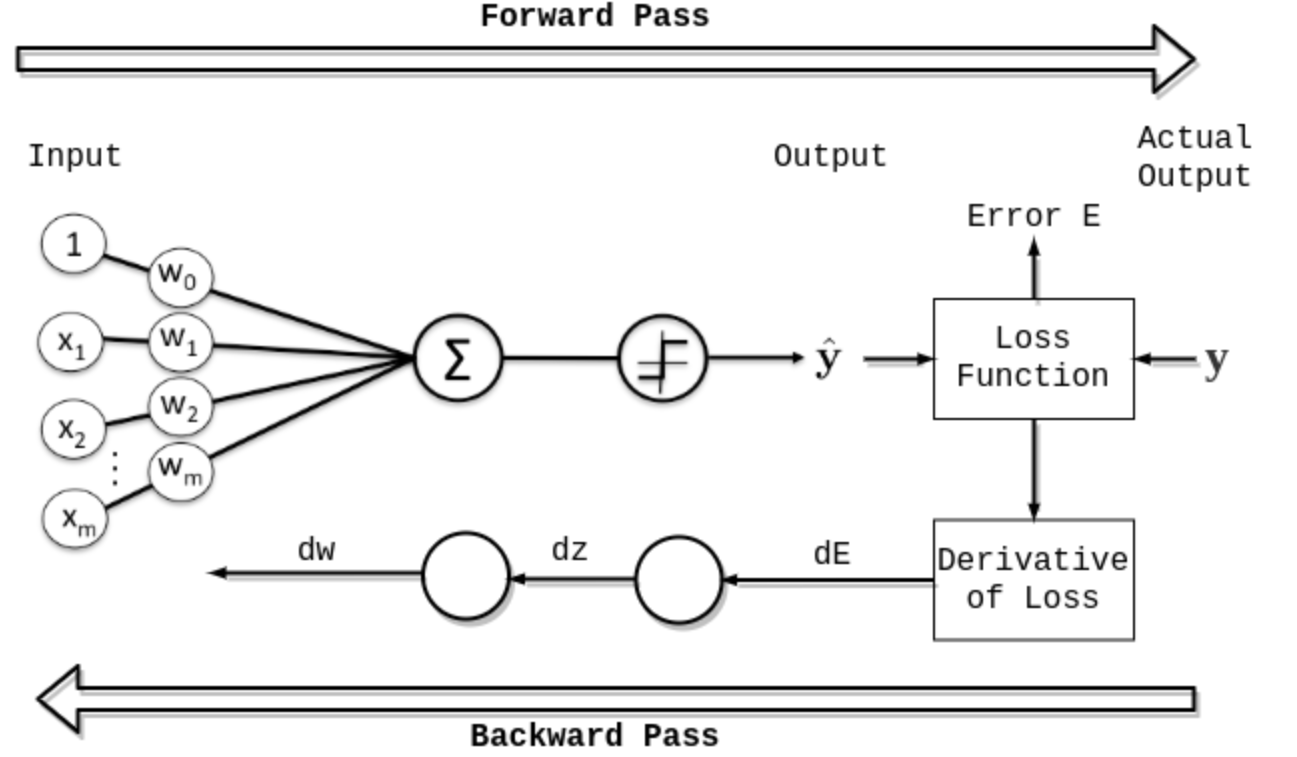
\includegraphics[width=0.8\textwidth]{imatges/preliminaries/front-and-back-prop.png}
    \caption[Forward Propagation and Backward Propagation]{\textit{Forward Propagation and Backward Propagation. Illustration by baeldung}}
{\label{fig:forward-and-back-propagation}}
\end{figure}


\subsection{Forward Propagation}

Forward propagation refers to the process of computing the output of a neural network given an input or a batch of inputs. During forward propagation, the input data flows through the network's layers in a sequential manner, from the input layer to the output layer. Each layer performs a series of computations, typically involving linear transformations (such as matrix multiplications) followed by activation functions. \\

As the data flows forward through the network, intermediate outputs, also known as activations or feature maps, are computed at each layer. These activations are then passed on as inputs to the subsequent layers until the final output is produced. The forward propagation process essentially calculates the predicted output of the network for a given input.

\subsection{Backward Propagation}

Backward propagation, short for backward propagation of errors, is the process of computing the gradients of the network's parameters with respect to a loss function. These gradients indicate the sensitivity of the network's output to changes in its parameters and are used to update the parameters during the training process. \\

The backward propagation algorithm starts from the final output of the network and propagates the error gradients backward through the network's layers. It computes the gradients layer by layer using the chain rule of calculus. The gradients quantify how each parameter contributed to the overall error of the network and provide information on how to adjust the parameters to reduce the error.


\section{Under-fitting vs Over-fitting}

Under-fitting is a prevalent challenge in machine learning, occurring when the model fails to establish a meaningful relationship between the input and target variable. Insufficiently capturing the features of the data results in increased errors in both the training and unseen data samples. \\

Over-fitting is also a prevalent challenge in machine learning but it is really common in deep learning algorithms. Deep learning models try to fit the training data entirely and ends up memorizing the data patterns and the noise/random fluctuations. These models fail to generalize and perform well in the case of unseen data scenarios, defeating the model's purpose. \\

\begin{figure}[H]
\centering
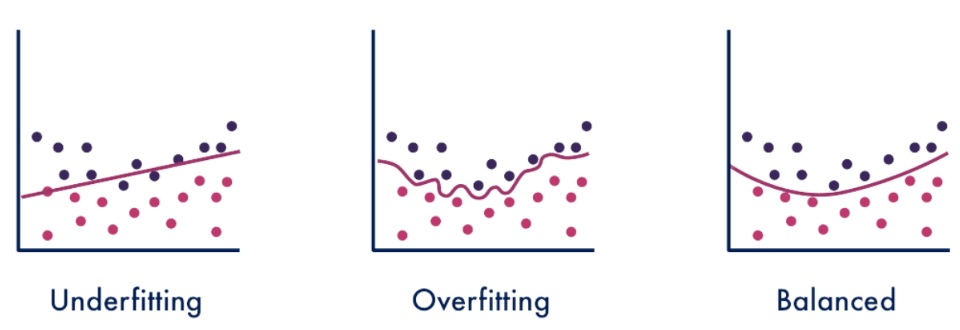
\includegraphics[width=0.8\textwidth]{imatges/preliminaries/over-under-base.jpg}
\caption[Fitting Scenarios]{\textit{Fitting Scenarios. Illustration by towardsdatascience}}
{\label{fig:underfitting-overfitting-goodfitting}}
\end{figure}

\section{Strategies to Combat Over-fitting}

There are lot of strategies to combat over-fitting, in this section there is presented only those used in the project. \\

\subsection{Early Stopping}

Early Stopping involves monitoring the model's performance on a validation dataset during training. If the performance stops improving or starts deteriorating, the training process is stopped early. By doing this, early stopping helps find the optimal balance between model complexity and generalization, ensuring the model doesn't become overly specialized to the training data and does not performs well on unseen data. \\

\begin{figure}[H]
\centering
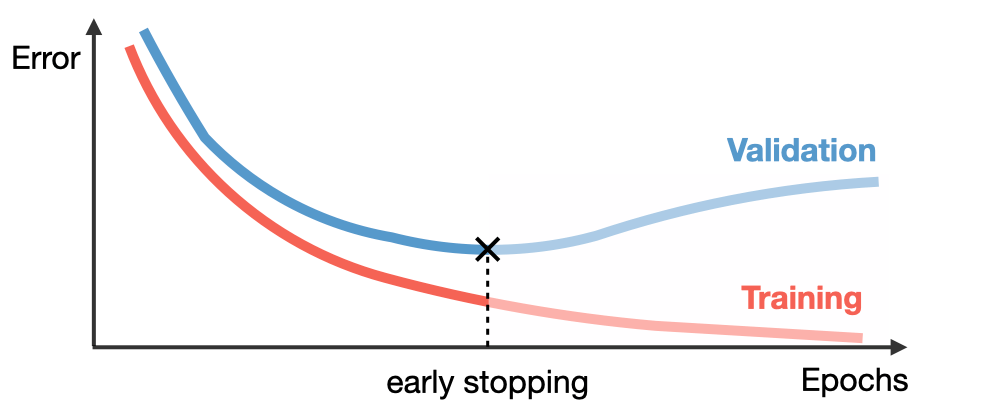
\includegraphics[width=0.7\textwidth]{imatges/preliminaries/early-stop.png}
\caption[Early Stopping]{\textit{Early Stopping. the vertical doted line represents the point where the early stop mechanism should have been triggered. Illustration by wandb}}
{\label{fig:early-stop}}
\end{figure}

\subsection{Learning Rate Scheduling}

The learning rate is a hyper-parameter in machine learning that determines the step size at which a model's parameters are updated during the optimization process. In most optimization algorithms, such as gradient descent, the learning rate controls how quickly or slowly the model learns from the training data. \\

There are various approaches in learning rate scheduling, bellow you'll find the scheduling used in the thesis.

\begin{itemize}
    \item \textbf{Learning Rate Decay}

    This learning rate scheduling works gradually reducing
    the learning rate over time or in response to certain conditions. \\

    A smaller learning rate allows the model to fine-tune its parameters more cautiously,
    preventing it from aggressively fitting to noisy or irrelevant patterns in the training data.
    A smoother or an agresive adjustment helps the model converge to a better generalize solution,
    reducing the risk of over-fitting. \\

    There are varius scheduler policies that we can follow to make the learning rate decay over
    the epochs. For instance, in \textit{Figure \ref{fig:learning-rate-decay-cosine-annealing}} follows the \textit{Cosine Annealing Learning Rate} scheduler, yet
    \textit{Figure \ref{fig:learning-rate-decay-step}} follows the \textit{Step Learning Rate} scheduler.

    \begin{figure}[H]
    \centering
    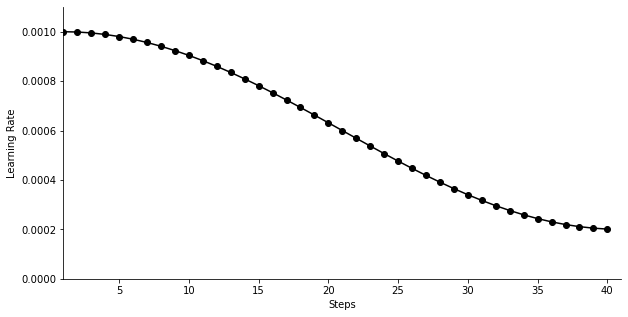
\includegraphics[width=0.6\textwidth]{imatges/preliminaries/cosinus-scheduler.png}
    \caption[Cosine Annealing Learning Rate Scheduler]{\textit{Cosine Annealing Learning Rate Scheduler. A learning rate decay scheduler with smoother behavior.
      Illustration by Author}}
    {\label{fig:learning-rate-decay-cosine-annealing}}
    \end{figure}

    \begin{figure}[H]
    \centering
    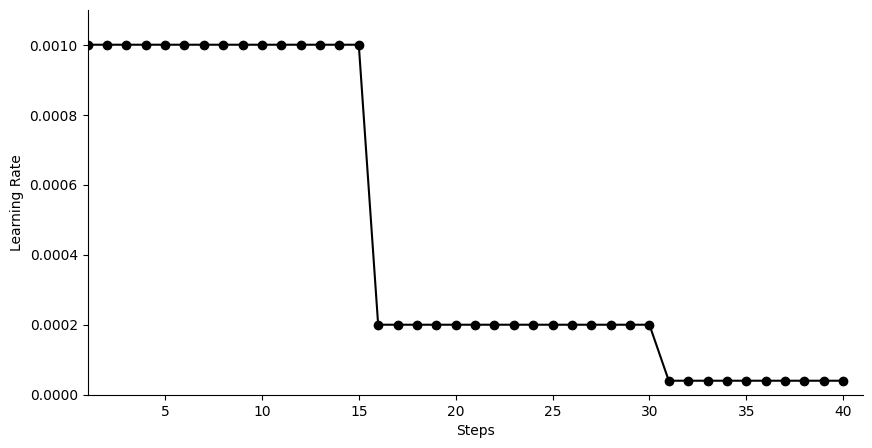
\includegraphics[width=0.6\textwidth]{imatges/preliminaries/step-scheduler.png}
    \caption[Step Learning Rate Scheduler]{\textit{Step Learning Rate Scheduler. A learning rate decay scheduler with
      and agresive behavior. Illustration by Author}}
    {\label{fig:learning-rate-decay-step}}
    \end{figure}

    \newpage

    \item \textbf{Cycling Learning}

    Cyclic learning rate scheduling is popular for
    faster convergence and improved generalization.
    By cycling the learning rate, models explore diverse loss landscape regions, escaping local minima for better optima.
    Variations like triangular and cosine annealing alternate or smoothly transition
    between lower and upper bounds. This approach adds variation and exploration to optimization, enhancing model performance and convergence. \\

    As well as in learning rate decay, there are various scheduler with it's own policy. \textit{Figure \ref{fig:cycling-rate-decay}} is
    a representation of a \textit{Cosine Annealing Warm Restart} scheduler.
    \begin{figure}[H]
    \centering
    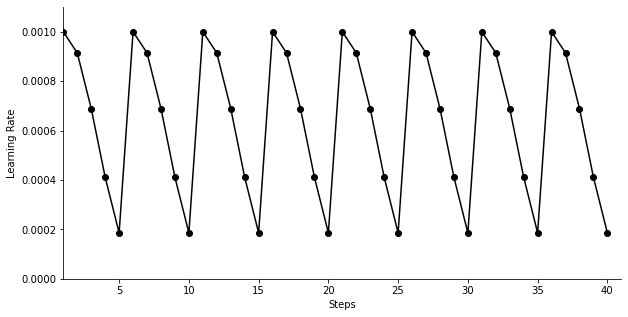
\includegraphics[width=0.6\textwidth]{imatges/preliminaries/CosineAnnealingWarmRestarts-scheduler.png}
    \caption[Cosine Annealing Warm Restart]{\textit{Cosine Annealing Warm Restart. A cosinus cycling learning scheduler.
   Illustration by Author}}
    {\label{fig:cycling-rate-decay}}
    \end{figure}
\end{itemize}

\newpage

\subsection{Dropout}

Dropout is a regularization method \cite{DropoutPaper}. The idea behind dropout is to prevent overfitting and improve generalization in neural networks by randomly "dropping out" or deactivating a fraction of the neurons during each training iteration. \\

By randomly dropping out neurons, the network becomes more robust and less sensitive to the precise configuration of any single neuron. It forces the network to learn redundant representations and prevents co-adaptation.

\begin{figure}[H]
\centering
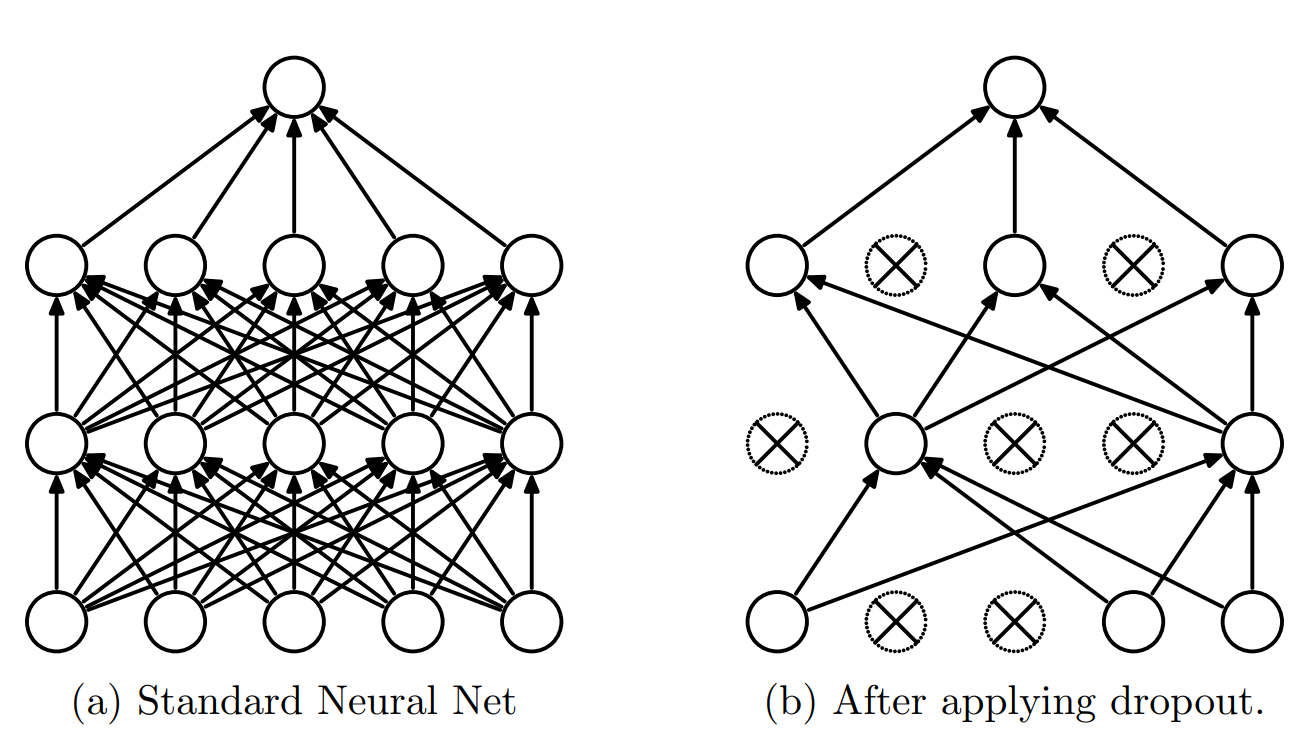
\includegraphics[width=10cm]{imatges/preliminaries/dropout.png}
\caption[Dropout]{\textit{Dropout Neural Net Model. \textbf{Left}: A standard neural net with 2 hidden layers. \textbf{Right}:
An example of a thinned net produced by applying dropout to the network on the left.
Crossed units have been dropped. Illustration by Srivastava}}
{\label{fig:dropout}}
\end{figure}

\section{Train, Validation and Test Sets}

The primary method employed to validate the models involves dividing the original dataset into three subsets using the Holdout set scheme, see \textit{Figure \ref{fig:holdout-test-scheme}}. The percentages applied to divide to the ISIC dataset used for training is 80\%, for validation 10\% and for testing 10\%. \\

Bellow there are the explanation of each dataset and the propose of all of them.

\begin{itemize}

  \item \textbf{Training Set}

This subset is utilized during the training phase of the model.

\item \textbf{Validation Set}

This subset was employed to apply trained models to new, unseen examples and evaluate the model's performance. It also aids in selecting the model that best matches the validation set by minimizing the classifier One vs Rest metric in predictions.

\item \textbf{Test Set}

Comprising non-observed data examples, this set is used to assess the performance of the chosen model. It helps determine if further optimization is required and which techniques should be applied next. Alternatively, it aids in deciding whether to select an alternative model.


\begin{figure}[H]
\centering
\begin{adjustbox}{width=0.8\textwidth, trim={0cm 0.5cm 0cm 0.5cm}, clip}
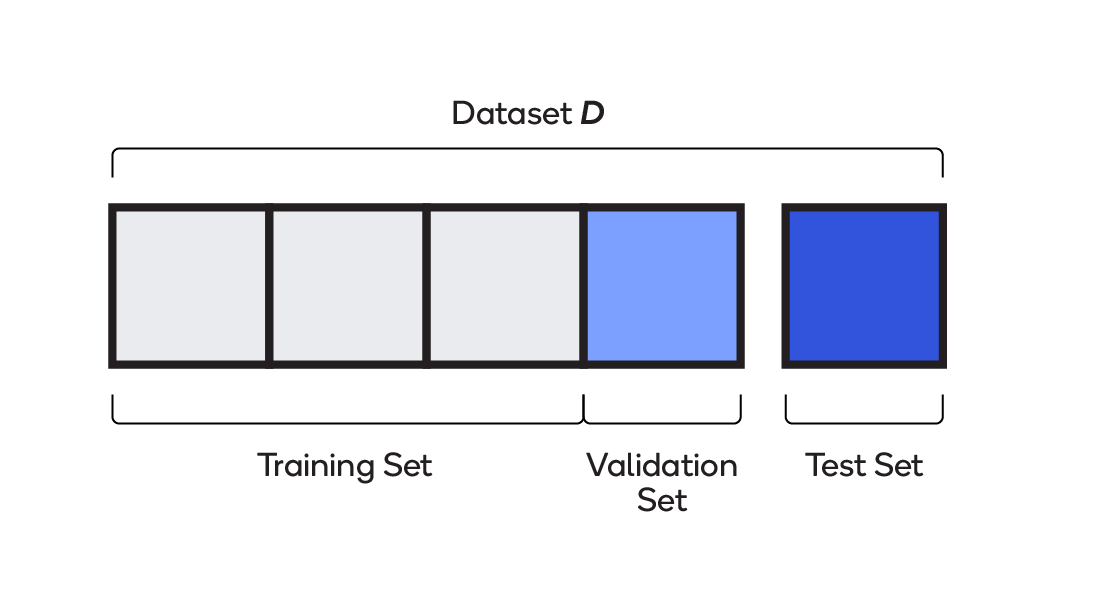
\includegraphics[\textwidth]{imatges/preliminaries/train-test-validation-sets.png}
\end{adjustbox}
\caption[Holdout Test Scheme]{\textit{Holdout Test Scheme. Illustration by Qualcomm}}
{\label{fig:holdout-test-scheme}}
\end{figure}

\end{itemize}

\newpage

\section{Data Augmentation}

Data augmentation encompasses various techniques utilized to expand the dataset by introducing modifications, thereby increasing the number of examples. Its purpose is not only to enlarge the dataset but also to enhance its diversity. By acting as a regularizer, data augmentation aids in mitigating overfitting during machine learning model training.

\begin{figure}[H]
\centering
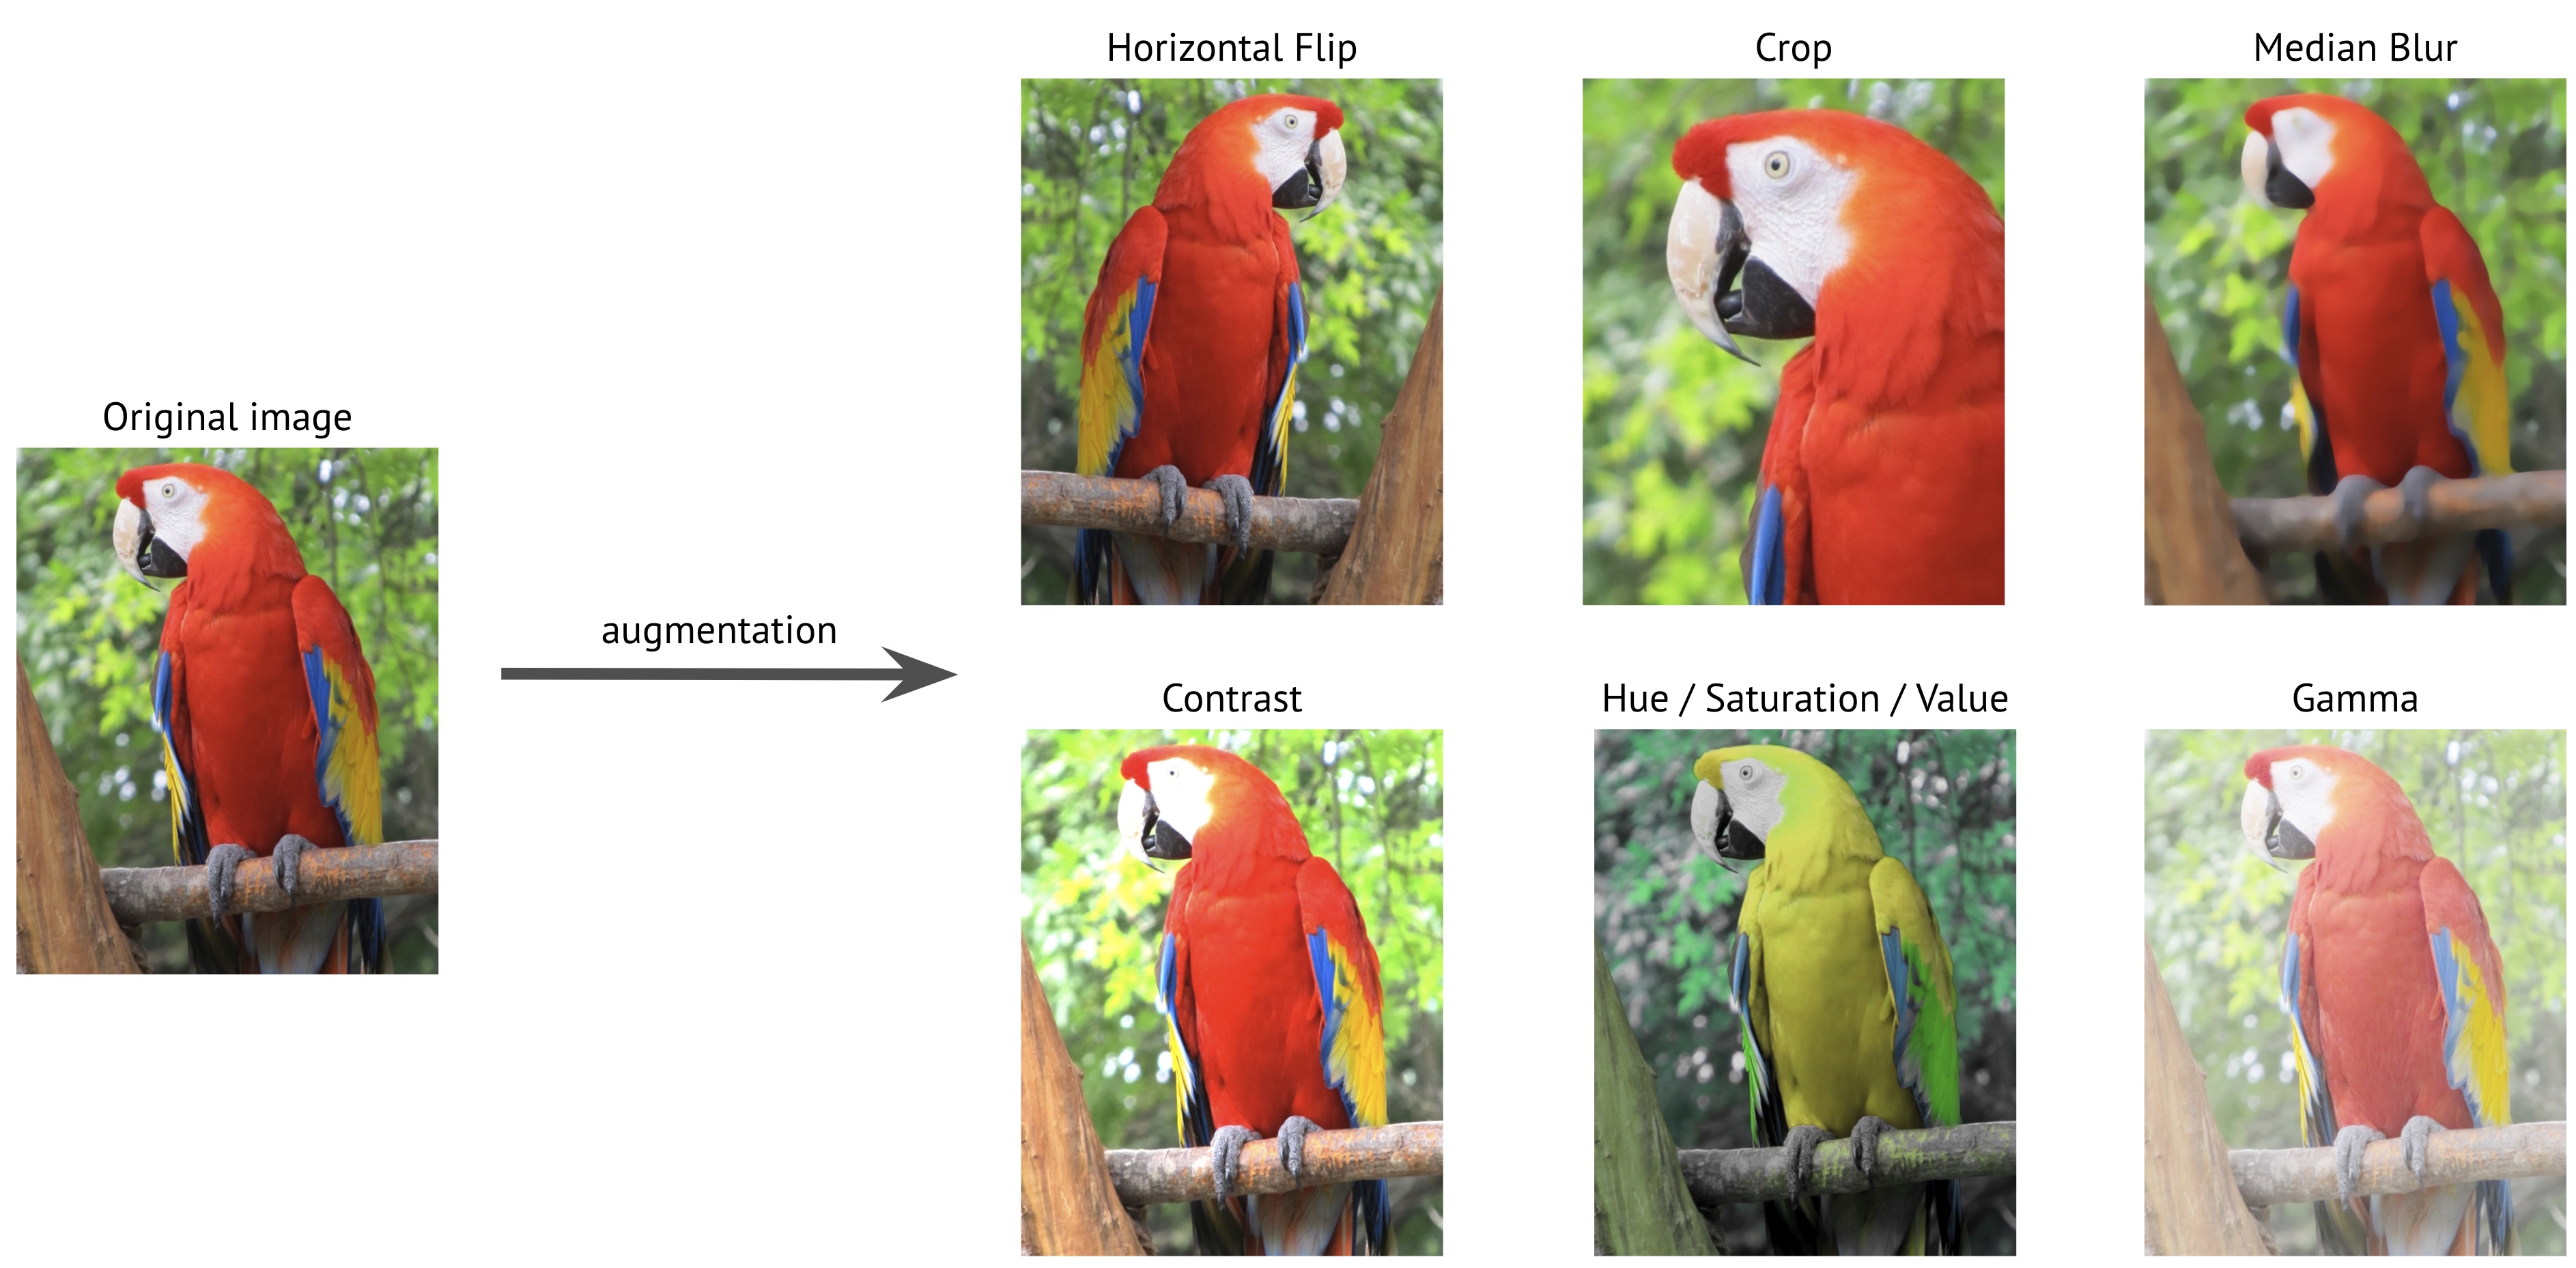
\includegraphics[width=0.7\textwidth]{imatges/preliminaries/augmentation.jpg}
\caption[Data Augmentation]{\textit{Data Augmentation. Illustration by Albumentations}}
{\label{fig:augmentation}}
\end{figure}


\section{Test-Time Augmentation}

Test-time augmentation (TTA) is used during the testing or inference phase of a machine learning model. TTA generates multiple augmented versions of test samples to obtain diverse predictions. By obtaining predictions from these augmented samples and combining them, TTA mimics the behavior of an ensemble of models.

\begin{figure}[H]
\centering
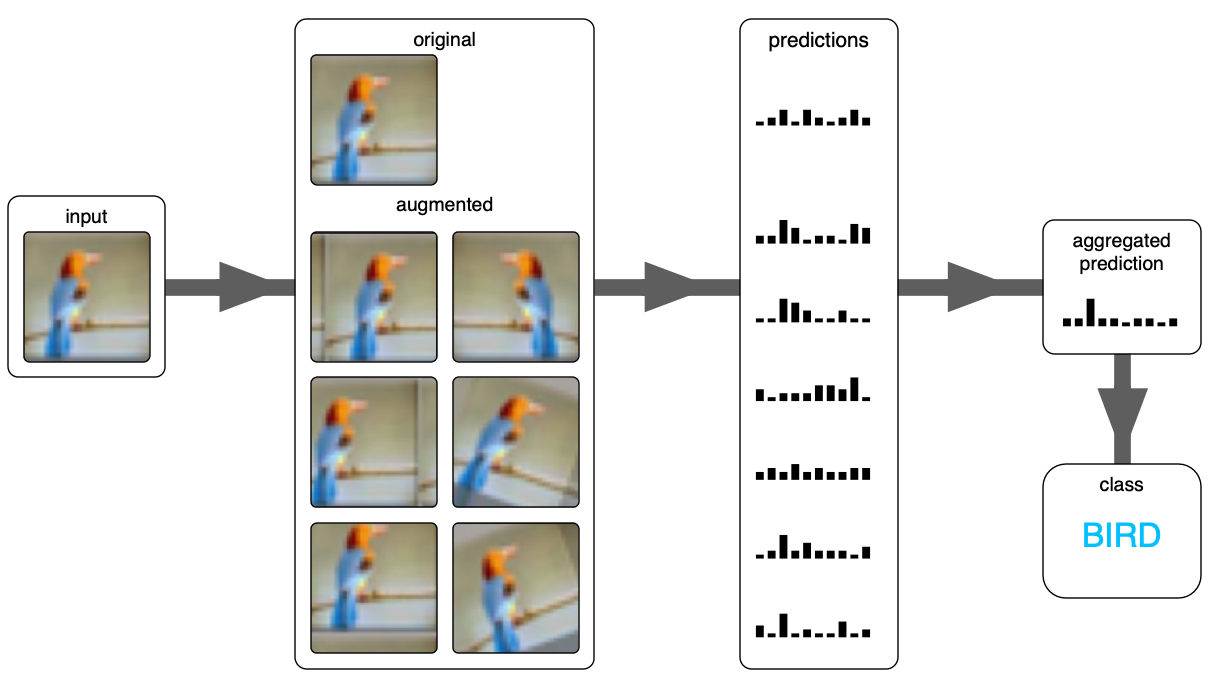
\includegraphics[width=0.8\textwidth]{imatges/preliminaries/tta.png}
\caption[Test-Time Augmentation]{\textit{Test-Time Augmentation. Illustration by stepup.ai}}
{\label{fig:tta}}
\end{figure}

\newpage

\section{ResNet}

ResNet, short for "Residual Network," is a deep convolutional neural network (CNN) architecture that was introduced in 2015 by researchers from Microsoft Research \cite{ResNetPaper}. It revolutionized the field of deep learning by addressing the challenge of training very deep neural networks. \\

The main problem encountered when training deep neural networks is the degradation problem, where the accuracy of the model saturates and then starts to decline rapidly as the network depth increases. This degradation occurs due to the difficulty of optimizing the network's parameters and the vanishing gradient problem, where gradients become extremely small during backpropagation, making it difficult for the network to learn effectively. \\

ResNet tackled this problem by introducing the concept of residual learning. The key idea is to use "skip connections" or "identity mappings" that allow the network to learn residual functions. Instead of trying to learn the underlying mapping directly, ResNet models learn the residual between the desired mapping and the input. \\

By introducing these skip connections, ResNet models can effectively "skip" one or more layers during training, allowing information to flow more easily through the network. This mitigates the degradation problem and enables the training of extremely deep networks (e.g., hundreds of layers) without suffering from diminishing accuracy. \\

In ResNet, each layer of the network contains a residual block. A residual block consists of multiple convolutional layers followed by batch normalization and activation functions. The input to a residual block is added to its output through a skip connection, which directly connects the input to the output. This allows the network to learn the residual information, or the difference between the input and the desired output, making it easier for the network to learn the underlying mapping.  \\

There are various architectural variants or "flavors" of ResNet, including {\tt ResNet-152}, {\tt ResNet-101}, {\tt ResNet-50}, {\tt ResNet-34}, and {\tt ResNet-18}. The number following the name of each ResNet variant indicates the number of inner layers present in the architecture.

\newpage

As evident from \textit{Figure \ref{fig:resnet}}, it can be observed that ResNet architectures with a greater number of layers tend to exhibit higher accuracy. However, it is important to note that this improvement in accuracy comes at the expense of having a significantly larger number of parameters to train.


\begin{figure}[H]
\begin{adjustbox}{width=\textwidth, trim={0pt 0pt 1cm 0pt}, clip}
\centering
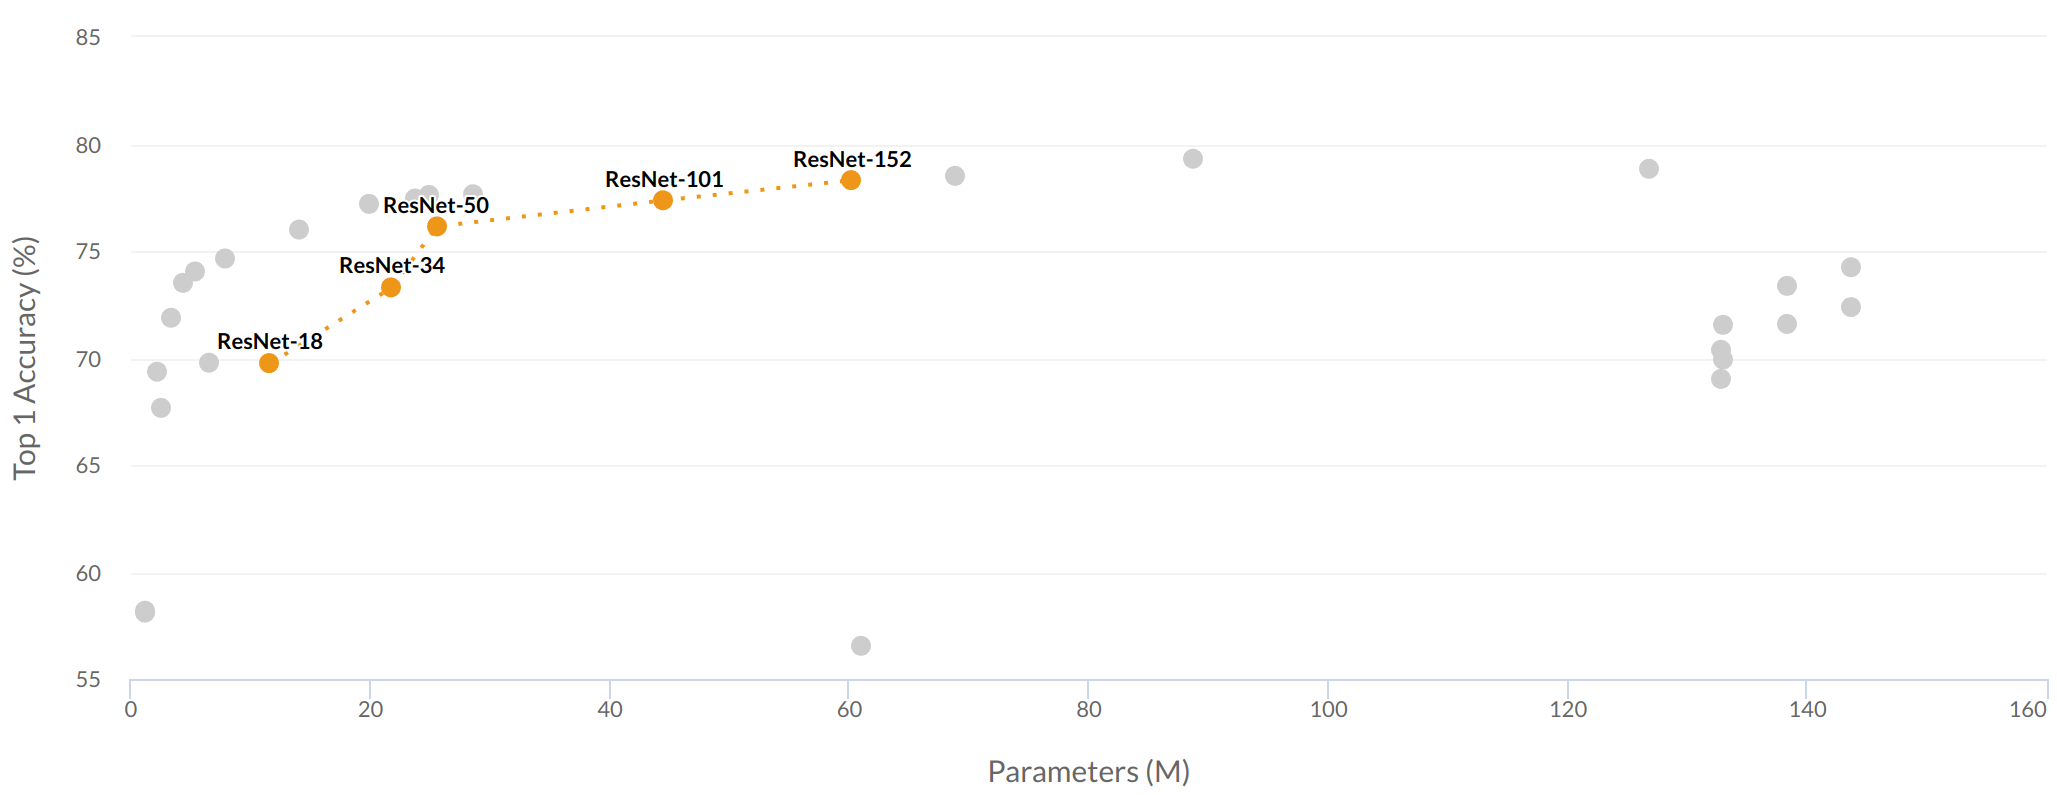
\includegraphics[width=\textwidth]{imatges/preliminaries/ResNetImageNet.png}
\end{adjustbox}
\caption[ResNet "flavors" Results on ImageNet]{\textit{ResNet "flavors" Results on ImageNet. Illustration by paperswithcode}}
{\label{fig:resnet}}
\end{figure}

To accurately assess the performance of each ResNet architecture, refer to the \textit{Table \ref{table:resnet}}, which provides the accuracy achieved on the ImageNet dataset along with the corresponding number of trainable parameters in millions.

\begin{table}[H]
\centering
\begin{tabular}{lcc}
\toprule
\textbf{Model} & \textbf{Accuracy} & \textbf{Parameters} \\
 \midrule
ResNet-152 & 78.31\% & 60.2M \\
ResNet-101 & 77.37\% & 44.5M \\
ResNet-50 & 76.15\% & 25.6M \\
ResNet-34 & 73.30\% & 21.8M \\
ResNet-18 & 69.76\% & 11.7M \\ \bottomrule
\end{tabular}
\caption[Accuracy Achieved on ImageNet and Trainable Parameters of Each ResNet.]
 {\textit{Accuracy Achieved on ImageNet and Trainable Parameters of Each ResNet.
  Each image in the ImageNet dataset is associated with 1 of 1,000 classes. Table by paperswithcode}}
{\label{table:resnet}}
\end{table}

\section{Micro-services Architecture}

A micro-services architecture is a software design approach that structures an application as a collection of small, independent services, each running in its own process and communicating with each other through lightweight mechanisms. This architecture promotes scalability, modularity, and flexibility. \\

The present thesis consists of two services: an API and a UI. These services are built using different frameworks and programming languages.


\section{Inference API}

The inference API service focuses on handling the back-end logic and data processing.
It exposes a well-defined API that allows user to interact with the trained models. \\

The end-points that the present thesis API service support are explained in \textit{Section \ref{cap:result}}.

\section{Containerization}

Containerization is a technology that allows applications and their dependencies to be packaged into isolated, lightweight containers. These containers provide an encapsulated runtime environment, ensuring that the application runs consistently across different systems. \\

Containers are created from container images, which are self-contained packages containing the application's code, dependencies, libraries, and configurations. Images serve as the blueprint for creating containers. They can be shared, versioned, and easily deployed on various platforms. \\

Frameworks such as Docker and Podman, provide tools and services to build, manage, and run containers. These frameworks utilize underlying virtualization technologies to create and manage isolated environments. These environments, called containers, offer resource isolation and ensure that applications run consistently across different computing environments.

\section{Platform Deployment}

To distribute the containerized API and UI services easily to professionals, there are several solutions available. In this thesis, I propose the creation of a shell script that performs the following steps:

\begin{itemize}
  \item Creates a directory in the system's home directory to download the source code and artifacts.
  \item Clones the source code repository from GitHub.
  \item Moves the encapsulated Python packages into the API source code.
  \item Builds the API image.
  \item Builds the UI image.
  \item Clones the artifacts from GitLab.
  \item Activates the services using a Docker Compose file, which starts the containers with their configurations based on the previously built images.
\end{itemize}

By following this approach, professionals can easily distribute the containerized services by running the provided shell script.


\chapter{Studies and Decisions}
\label{cap:studies_and_decisions}

This chapter is dedicated to exploring the essential tools required for the project's development and understanding their significance. The initial section of this chapter focuses on delineating the functional and non-functional requirements that the system must fulfill. Subsequently, the second part identifies and elucidates the selected technologies for the project.

\section{System Requirement}

This section explores the necessary requirements for detecting melanoma. It is important to distinguish between the final system and the work involved in its development. Constructing and training a Convolutional Neural Network (CNN) requires substantial computational power, sophisticated libraries, and often a significant amount of time. However, once the model has been trained and saved, it can be readily used. Typically, the response time inferring is within seconds. Yet the inference time of the models is few we also need to take into account the time wasted in the HTTP request and the time wasted in showing the results. \\

The requirements can be classified into two categories:

\begin{itemize}
    \item \textbf{Functional requirements}

    Functional requirements pertain to the capabilities that the product must possess to fulfill specific user needs.

    \item \textbf{Non-functional requirements}

    Non-functional requirements encompass aspects such as usability, performance, reliability.
\end{itemize}

\newpage

\vspace{0.5cm}
\textbf{Functional requirements} \\

The functional requirements of the system are:

\begin{itemize}
    \item The objective is to classify whether a single image or a set of images, specifically from a dermoscopy, contains a melanoma or not. The classification task is binary, aiming to determine the presence or absence of melanoma.

    \item Expose models through an API that can classify whether an image or a set of images contains melanoma or not. The API should not only provide the classification results but also offer additional information such as the specific model used and the probabilities associated with the prediction..

    \item A user-friendly interface (UI) is implemented to facilitate loading of images and communicate with the API via the HTTP protocol for image inference. The UI should display the results of the selected model for the bulk of loaded images.

    \item Create images of each service, to distribute the services using container technology.
\end{itemize}

\vspace{0.5cm}
\textbf{Non-functional requirements} \\

For training models, Jupyter Notebook, Python3, and Anaconda are used, ensuring compatibility with any computer to run the code and classify images. Sufficient RAM is required to handle the desired images effectively. \\

Since the API and UI services are containerized, any container management tool such as Docker or Podman can be used, providing the necessary environment to work with containers.

\newpage

\section{Hardware}

The hardware used for the thesis encompassed a range of machines. The primary development machine employed was a laptop with limited performance. Additionally, a machine provided by Google was utilized within the Google Colab environment for training models that did not require high computational capabilities. Furthermore, for a week of work at the VICOROB laboratory, a separate machine was utilized specifically for training models with more extensive data augmentation requirements, necessitating higher computational resources. \\

\textit{Table \ref{table:dev-machine}, \ref{table:google-machine}, and \ref{table:vicorobot-machine}} provide an overview of the characteristics of the machines employed for the project. Each of these machines had its own specific use, and it is recommended to select the an appropriate machine based on specific needs.

\begin{table}[H]
	\centering
	\begin{tabular}{cc}
		\toprule
		\multicolumn{2}{c}{\textbf{Development Machine}} \\
		\midrule
		OS & Fedora Linux 38 \\
		CPU & Intel i5-8250U \\
		GPU & Intel UHD Graphics 620 \\
		RAM & 8GB \\
		Disk & 225GB \\
		\bottomrule
	\end{tabular}
  \caption[Development Machine Metrics.]
  {\textit{Development Machine Metrics.
  This machine was only used for programming and searching thesis information.
  Table by Author}}
	\label{table:dev-machine}
\end{table}


\begin{table}[H]
	\centering
	\begin{tabular}{cc}
			\toprule
			  \multicolumn{2}{c}{\textbf{Google Machine}} \\
			  \midrule
			  OS & Ubuntu 20.04.6 LTS \\
			  CPU & Intel Xeon \\
			  GPU & Tesla T4, 16GB \\
			  RAM & 12GB \\
			  Disk & 125GB \\
			  \bottomrule
\end{tabular}
\caption[Google Machine Metrics.]
  {\textit{Google Machine Metrics.
  Note that this machine was used to train models that take at most a pair of hours to accomplish the training.
  Table by Author}}
{\label{table:google-machine}}
\end{table}

\newpage

\begin{table}[H]
\centering
\begin{tabular}{cc}
	 \toprule
		\multicolumn{2}{c}{\textbf{VICOROB Machine}} \\
		\midrule
		OS & Ubuntu 20.04.2 LTS \\
		CPU & Intel(R) Xeon(R) Silver \\
		GPU & A100, 80GB\\
		RAM & 396GB \\
		Disk & 6.3T \\
		\bottomrule
\end{tabular}
\caption[VICOROB Machine Metrics.]
  {\textit{VICOROB Machine Metrics.
  This machine was used to train models that required high computational resources because of data augmentation.
  Table by Author}}
{\label{table:vicorobot-machine}}
\end{table}

\section{Software}

In order to establish and operate the CAD infrastructure, it was crucial to establish separate environments for creating the services and training the models, ensuring that all the required packages were included. The detailed instructions for setting up these distinct environments can be found in \textit{Appendix \ref{appendix:appendix_a}}. Additionally, \textit{Appendix \ref{appendix:appendix_b}} provides a guide on deploying and activating the services within the CAD infrastructure. \\

The following pages will outline and provide detailed descriptions of each tool utilized throughout the thesis. These tools played a crucial role in various aspects, including the training process, creation of services such as user interface (UI) and application programming interface (API), deployment of these services with trained models, management of the source code, and comprehensive documentation. Each tool's significance and contribution to the thesis will be thoroughly explained, shedding light on their specific functionalities and importance in the research project.

\newpage

\vspace{0.5cm}
\textbf{Python 3.9} \\

Python (\textit{Figure \ref{fig:python-logo}}) is a high-level, interpreted programming language known for its simplicity and readability. It was created by Guido van Rossum and released in 1991. Its design philosophy emphasizes code readability with the use of significant indentation. \\

Python is an ideal choice for machine learning and AI-based projects due to several advantages. These include its simplicity and consistency, access to excellent libraries and frameworks specifically designed for AI and ML, flexibility, platform independence, and a large and supportive community.

\begin{figure}[H]
\centering

\includegraphics[width=0.15\textwidth]{imatges/studies_and_decisions/python-logo-only.png}
\caption[Python Logo]{\textit{Python Logo. Illustration by Python Software Foundation}}
{\label{fig:python-logo}}
\end{figure}

\vspace{0.5cm}
\textbf{Anaconda} \\

Anaconda (\textit{Figure \ref{fig:anaconda-logo}}) is a widely used open-source distribution of the Python programming language. It simplifies the management and deployment of data science and machine learning environments. With Anaconda, you can easily install and manage Python packages using the conda package management system. It also provides tools for creating isolated environments to ensure consistent dependencies and package versions.

\begin{figure}[H]
\centering
  \begin{adjustbox}{trim=0cm 1cm 0cm 1cm, clip}

\includegraphics[width=0.5\textwidth]{imatges/studies_and_decisions/anaconda-logo.png}
\end{adjustbox}
\caption[Anaconda Logo]{\textit{Anaconda Logo. Illustration by Anaconda}}
{\label{fig:anaconda-logo}}
\end{figure}


\vspace{0.5cm}
\textbf{Jupyter Notebook} \\

Jupyter Notebook (\textit{Figure \ref{fig:jupyter-logo}}) is an open-source web application that allows to create and share interactive documents containing live code, visualizations, and text. It provides an environment for data analysis, visualization, and prototyping. With Jupyter Notebooks, you can write and execute code in individual cells, making it easy to experiment and iterate. It supports multiple programming languages such as Python, R and Haskell.

\begin{figure}[H]
\centering

\includegraphics[width=0.2\textwidth]{imatges/studies_and_decisions/jupyter-notebook.png}
\caption[Jupyter Notebook Logo]{\textit{Jupyter Notebook Logo. Illustration by Jupyter.org}}
{\label{fig:jupyter-logo}}
\end{figure}

\vspace{0.5cm}
\textbf{CUDA} \\

CUDA (\textit{Figure \ref{fig:cuda-logo}}), which stands for Compute Unified Device Architecture, is a parallel computing platform and programming model developed by NVIDIA. It enables developers to leverage the power of NVIDIA GPUs (Graphics Processing Units) for high-performance computing tasks. \\

CUDA has gained widespread adoption in the scientific and computational research communities due to its ability to leverage the computational power of GPUs. It has become an essential tool for accelerating a wide range of applications, from physics simulations and computational biology to data analytics and artificial intelligence.

\begin{figure}[H]
\centering
\begin{adjustbox}{trim=0cm 0.25cm 0cm 0.5cm, clip}

\includegraphics[width=0.325\textwidth]{imatges/studies_and_decisions/nvidia-cuda.jpg}
\end{adjustbox}
\caption[CUDA Logo]{\textit{CUDA Logo. Illustration by Nvidia Corporation}}
{\label{fig:cuda-logo}}
\end{figure}

\vspace{0.5cm}
\textbf{PyTorch} \\

PyTorch (\textit{Figure \ref{fig:pytorch-logo}}) is an open-source machine learning framework widely used for deep learning tasks. It provides a flexible and dynamic approach to building and training neural networks. PyTorch stands out for its integration of GPU acceleration, enabling efficient computations using NVIDIA GPUs. \\

PyTorch offers a high-level API called torchvision, which simplifies common computer vision tasks such as image classification, object detection, and image generation. It also integrates with other libraries and tools in the Python ecosystem, making it easy to combine PyTorch with popular frameworks like NumPy, SciPy, and pandas.

\begin{figure}[H]
\centering

\includegraphics[width=0.325\textwidth]{imatges/studies_and_decisions/pytorch-logo.png}
\caption[PyTorch Logo]{\textit{PyTorch Logo. Illustration by PyTorch.org}}
{\label{fig:pytorch-logo}}
\end{figure}

\vspace{0.5cm}
\textbf{OpenCV} \\

OpenCV (Open Source Computer Vision Library), is a popular open-source computer vision and image processing library. It provides a wide range of functions and algorithms for tasks such as image and video processing, object detection and tracking, feature extraction, and more. \\

OpenCV (\textit{Figure \ref{fig:opencv-logo}}) allows developers to read, write, and manipulate images and videos efficiently. The library offers various image processing functions, including filtering, resizing, color conversion, and geometric transformations.

\begin{figure}[H]
\centering
\begin{adjustbox}{trim=1cm 1cm 1cm 1cm, clip}

\includegraphics[width=0.7\textwidth]{imatges/studies_and_decisions/OpenCV-logo.png}
\end{adjustbox}
\caption[OpenCV Logo]{\textit{OpenCV Logo. Illustration by OpenCV Team}}
{\label{fig:opencv-logo}}
\end{figure}


\vspace{0.5cm}
\textbf{Albumentations} \\

Albumentations (\textit{Figure \ref{fig:albumentations-logo}}) is an open-source Python library for image augmentation in machine learning and computer vision tasks. It provides a wide range of transformations and optimizations to enhance training data, improving the performance and generalization of machine learning models. With high-performance implementation and seamless integration with popular frameworks, Albumentations is widely used for efficient and customizable image augmentation.

\begin{figure}[H]
\centering

\includegraphics[width=0.13\textwidth]{imatges/studies_and_decisions/albumentations-logo.png}
\caption[Albumentations Logo]{\textit{Albumentations Logo. Illustration by Albumentations Team}}
{\label{fig:albumentations-logo}}
\end{figure}


\vspace{0.5cm}
\textbf{NumPy} \\

NumPy (\textit{Figure \ref{fig:numpy-logo}}) is a Python library for efficient numerical computing. It provides a powerful array object for manipulation and computation of multidimensional arrays. With optimized operations and support for broadcasting.

\begin{figure}[H]
\centering

\includegraphics[width=0.225\textwidth]{imatges/studies_and_decisions/numpy-logo.png}
\caption[NumPy Logo]{\textit{NumPy Logo. Illustration by NumPy Organazation}}
{\label{fig:numpy-logo}}
\end{figure}


\vspace{0.5cm}
\textbf{Pandas} \\

Pandas (\textit{Figure \ref{fig:pandas-logo}}) is a popular Python library for data manipulation and analysis. It provides data structures and functions to efficiently work with structured data, such as tabular data and time series. Pandas' key features include its DataFrame object, which allows for easy handling of data, indexing, filtering, and aggregation operations. With its intuitive and powerful functionality, Pandas is widely used in data preprocessing, exploration, and analysis tasks.

\begin{figure}[H]
\centering

\includegraphics[width=0.3\textwidth]{imatges/studies_and_decisions/pandas-logo.png}
\caption[Pandas Logo]{\textit{Pandas Logo. Illustration by The pandas development team}}
{\label{fig:pandas-logo}}
\end{figure}


\vspace{0.5cm}
\textbf{Matplotlib} \\

Matplotlib (\textit{Figure \ref{fig:matplotlib-logo}}) is a widely-used Python library for creating static, animated, and interactive visualizations. It provides a flexible and comprehensive range of functions and tools for generating plots, charts, histograms, and more. Matplotlib allows customization of various aspects of visualizations, including colors, labels, titles, axes, and legends. With its extensive functionality and compatibility with NumPy arrays, Matplotlib is a go-to library for data visualization and presentation in Python.

\begin{figure}[H]
\centering

\includegraphics[width=0.45\textwidth]{imatges/studies_and_decisions/matplotlib-logo.png}
\caption[Matplotlib Logo]{\textit{Matplotlib Logo. Illustration by Matplotlib Organization}}
{\label{fig:matplotlib-logo}}
\end{figure}

\vspace{0.5cm}
\textbf{Seaborn} \\

Seaborn (\textit{Figure \ref{fig:seaborn-logo}}) is a Python data visualization library built on top of Matplotlib. It provides a high-level interface for creating attractive and informative statistical graphics. Seaborn simplifies the process of generating complex visualizations by offering a range of built-in functions for creating appealing plots, such as scatter plots, histograms, bar plots, and heatmaps. Seaborn is widely used for exploratory data analysis and presentation of statistical insights.

\begin{figure}[H]
\centering

\includegraphics[width=0.25\textwidth]{imatges/studies_and_decisions/seaborn-logo.png}
\caption[Seaborn Logo]{\textit{Seaborn Logo. Illustration by Seaborn Organization}}
{\label{fig:seaborn-logo}}
\end{figure}

\vspace{0.5cm}
\textbf{WandB} \\

Weights \& Biases (\textit{Figure \ref{fig:wandb-logo}}) is a machine learning experiment tracking and visualization platform. It offers a suite of tools to track, organize, and analyze machine learning experiments. With wandb, developers can log metrics, hyperparameters, and model checkpoints during training, making it easy to compare and analyze different experiments.

\begin{figure}[H]
\centering

\includegraphics[width=0.4\textwidth]{imatges/studies_and_decisions/wandb-logo.png}
\caption[Seaborn Logo]{\textit{Seaborn Logo. Illustration by Weights \& Biases Inc}}
{\label{fig:wandb-logo}}
\end{figure}

\vspace{0.5cm}
\textbf{FastAPI} \\

FastAPI (\textit{Figure \ref{fig:fastapi-logo}}) is a modern, high-performance web framework for building APIs with Python. It emphasizes simplicity, speed, and type annotations to create efficient and scalable web applications. FastAPI leverages Python's type hints for automatic request and response validation, enabling faster development and reducing the chances of introducing bugs. It provides asynchronous capabilities using Python's asyncio framework, allowing for high-concurrency and efficient handling of multiple requests. With its intuitive API declaration syntax and automatic generation of interactive documentation, FastAPI simplifies the process of building robust and well-documented APIs.

\begin{figure}[H]
\centering
\begin{adjustbox}{trim=0cm 0.25cm, clip}

\includegraphics[width=0.35\textwidth]{imatges/studies_and_decisions/fastapi-logo.png}
\end{adjustbox}
\caption[FastAPI Logo]{\textit{FastAPI Logo. Illustration by tiangolo}}
{\label{fig:fastapi-logo}}
\end{figure}

\vspace{0.5cm}
\textbf{JS} \\

JavaScript (\textit{Figure \ref{fig:js-logo}}) is a versatile programming language primarily used for client-side web development. It enables dynamic and interactive functionality on websites, allowing for real-time manipulation of HTML elements, handling user events, and modifying web page content.

\begin{figure}[H]
\centering
\begin{adjustbox}{trim=0cm 0cm, clip}

\includegraphics[width=0.15\textwidth]{imatges/studies_and_decisions/js-logo.png}
\end{adjustbox}
\caption[JS Logo]{\textit{JS Logo. Illustration by JS Organization}}
{\label{fig:js-logo}}
\end{figure}

\newpage

\vspace{0.5cm}
\textbf{SvelteKit} \\

SvelteKit (\textit{Figure \ref{fig:sveltekit-logo}}) is a high-performance JavaScript framework for building web applications. It uses a compiler-based approach, resulting in optimized applications with minimal overhead. It provides built-in routing, supports Server-Side Rendering (SSR) and Static Site Generation (SSG), and promotes component reusability. SvelteKit offers a developer-friendly environment, integrates well with APIs, and generates small bundles for faster loading times.

\begin{figure}[H]
\centering
\begin{adjustbox}{trim=0cm 0cm, clip}

\includegraphics[width=0.12\textwidth]{imatges/studies_and_decisions/sveltekit-logo.png}
\end{adjustbox}
\caption[SvelteKit Logo]{\textit{SvelteKit Logo. Illustration by WIKIPEDIA}}
{\label{fig:sveltekit-logo}}
\end{figure}

\vspace{0.5cm}
\textbf{Docker} \\

Docker (\textit{Figure \ref{fig:docker-logo}}) is an open-source platform for building and deploying applications in isolated containers. It simplifies application management, ensures portability across different environments, and provides isolation for enhanced scalability and security. With Docker, developers can package applications and their dependencies into lightweight, self-contained containers, making deployment and scaling more efficient.

\begin{figure}[H]
\centering
\begin{adjustbox}{trim=0cm 0cm, clip}

\includegraphics[width=0.4\textwidth]{imatges/studies_and_decisions/docker-logo.png}
\end{adjustbox}
\caption[SvelteKit Logo]{\textit{SvelteKit Logo. Illustration by WIKIPEDIA}}
{\label{fig:docker-logo}}
\end{figure}


\vspace{0.5cm}
\textbf{Podman} \\

Podman (\textit{Figure \ref{fig:podman-logo}}) is designed to manage containers and container images, offering features similar to Docker but with a focus on security and compatibility with industry standards. It allows you to build, run, and manage containers without the need for a separate daemon. \\

One key advantage of Podman is its rootless mode, which allows users to run containers as non-root, enhancing security and isolation. This eliminates the need for privileged access, making Podman a preferred choice for environments where running containers as non-root is required.

\begin{figure}[H]
\centering
\begin{adjustbox}{trim=0cm 0.25cm, clip}

\includegraphics[width=0.3\textwidth]{imatges/studies_and_decisions/podman-logo.png}
\end{adjustbox}
\caption[Podman Logo]{\textit{Podman Logo. Illustration by Red Hat}}
{\label{fig:podman-logo}}
\end{figure}

\vspace{0.5cm}
\textbf{Git} \\

Git (\textit{Figure \ref{fig:git-logo}}) is a distributed version control system used for tracking changes in software projects. It enables collaboration, allows for branching and merging, handles large projects efficiently, and provides robust backup options.

\begin{figure}[H]
\centering
\begin{adjustbox}{trim=0cm 0.25cm, clip}

\includegraphics[width=0.25\textwidth]{imatges/studies_and_decisions/git-logo.jpg}
\end{adjustbox}
\caption[Git Logo]{\textit{Git Logo. Illustration by Red Hat}}
{\label{fig:git-logo}}
\end{figure}

\vspace{0.5cm}
\textbf{GitHub \& GitLab} \\

Both GitHub (\textit{Figure \ref{fig:github-logo}}) and GitLab (\textit{Figure \ref{fig:gitlab-logo}}) serve as centralized platforms for hosting and managing Git repositories.

\begin{figure}[H]
\centering
\begin{adjustbox}{trim=0cm 0cm, clip}

\includegraphics[width=0.15\textwidth]{imatges/studies_and_decisions/github-mark.png}
\end{adjustbox}
\caption[GitHub Logo]{\textit{GitHub Logo. Illustration by GitHub}}
{\label{fig:github-logo}}
\end{figure}

\begin{figure}[H]
\centering
\begin{adjustbox}{trim=0cm 0cm, clip}
\includegraphics[width=0.15\textwidth]{imatges/studies_and_decisions/gitlab-logo.png}
\end{adjustbox}
\caption[GitLab Logo]{\textit{GitLab Logo. Illustration by GitLab}}
{\label{fig:gitlab-logo}}
\end{figure}

\vspace{0.5cm}
\textbf{LaTeX} \\

LaTeX (\textit{Figure \ref{fig:latex-logo}}) is a typesetting system used for creating high-quality documents, particularly those with mathematical equations and scientific content. It focuses on the structure and formatting of documents, allowing users to concentrate on content.

\begin{figure}[H]
\centering
\begin{adjustbox}{trim=0cm 0cm, clip}
\includegraphics[width=0.25\textwidth]{imatges/studies_and_decisions/latex-logo.png}
\end{adjustbox}
\caption[LaTeX Logo]{\textit{LaTeX Logo. Illustration by LaTeX}}
{\label{fig:latex-logo}}
\end{figure}


\chapter{Planning and Methodology}
\label{cap:plan}

\section{Feasibility Study}

Before initiating any project, it is of utmost importance to conduct a comprehensive analysis of relevant factors to gauge the likelihood of accomplishing successful outcomes. While estimating the complexity associated with developing, deploying, and maintaining machine learning (ML) systems is indeed a challenging task, it is essential to recognize that this project encompasses not only the research aspect but also significant software and infrastructure development. \\

This project requires a careful balancing act, as it involves dedicating efforts to both the research and practical implementation aspects. The development of robust software and infrastructure is crucial to support the successful integration of the deep learning models and ensure their efficient deployment and maintenance. This integration can be intricate and demanding, as it requires a deep understanding of both the ML algorithms and the software engineering principles. \\

In light of these additional dimensions, the study not only aims to evaluate the feasibility of utilizing deep learning techniques but also strives to address the complexities inherent in developing a well-rounded solution. Furthermore, the evaluation will consider the available data and resources to assess the potential of achieving satisfactory results.

\section{Technical Study}

The journey begins with research,
a dynamic element that evolves and gains strength through continuous investigation.
While it is impossible to guarantee the achievement of all objectives, the way we see it,
there are three fundamental pillars that must be addressed in advance. \\

\vspace{0.5cm}
\textbf{Defining the Use Case} \\

\textit{A perfect use case outlines a project that is precisely defined, quantifiable, attainable, and possesses clearly identified users and value.} \\

Academic researchers may find satisfaction in uncovering effective solutions that contribute to publications
and secure additional funding. Yet, this thesis aims to ensure the successful implementation of a Computer-Aided Diagnosis (CAD)
infrastructure specifically designed for classifying melanoma,
with the intention of deploying it in real-world scenarios we needed to look further than just the pure research. \\

\vspace{0.5cm}
\textbf{Equipment and Technical Knowledge} \\

Equipment and technical knowledge are interdependent and collectively contribute to the success of a machine learning project. \\

In a deep learning project, both the availability of suitable equipment and technical knowledge are essential. The correct equipment, including high performance computing resources and data collection devices, facilitates efficient data handling, prepossessing, model training, and deployment. Simultaneously, technical knowledge plays a vital role in effectively leveraging the available equipment. Understanding diverse machine learning algorithms and methodologies assists in selecting the most appropriate approaches for the problem at hand. Additionally, it is crucial to acknowledge the knowledge required to create other services that accompany the project. \\

\vspace{0.5cm}
\textbf{Importance of the Dataset} \\

The success of a project like this one depends not only on the quantity but also on the quality of the data. Data is essential for any deep learning model to learn effectively. Therefore, it is vital to invest time in
acquiring an optimal image data-set that possesses sufficient data volume, annotation, truth, and reusability. \\

For computer-based image recognition and analysis, high-quality data is necessary. The objective is to gather data from various patient populations to ensure that the data-set is diverse and accurately represents different disease states and outcomes. Often, healthcare organizations engage medical experts to review and label the data to prevent inaccurate labels and ensure the data-set's significance, as is the case in this project.

\section{Economical Study}

\vspace{0.5cm}
\textbf{Equipment Cost} \\

Equipment cost pertains to the expenditure incurred on hardware and software licenses necessary for the project. \\

The hardware and software used in the project are listed in the \textit{Table \ref{table:equipment_cost}}.

\begin{table}[H]
\centering
\begin{tabular}{lccc}
	 \toprule
    \textbf{Component} & \textbf{Units} & \textbf{Unit Price} & \textbf{Cost} \\
		\midrule
    Computer & 1 & \$800 & \$800 \\
    Software (Pytorch, Svelte, FastAPI, etc) & 1 & \$0 & \$0 \\
    Tesla T4, 16GB (GPU)* & 1 & \$2000 & \$2000 \\
    Nvidia A100, 80GB (GPU)* & 1 & \$15000 & \$15000 \\
		\bottomrule
\end{tabular}
\caption[The Cost of Components.]
  {\textit{The Cost of Components.
  Components marked with (*) were not paid for out of my own pocket; instead, they were borrowed from VICOROB or
  Google Services. Table by Author}}
{\label{table:equipment_cost}}
\end{table}

\vspace{0.5cm}
\textbf{Human Resources} \\

In this section, a hypothetical scenario is presented, illustrating multiple work profiles contributing to the project and the associated costs for each service. However, it is important to note that in reality, all tasks were performed by a single individual. \\

Below, the roles required to achieve the thesis are presented along with their explanations. \\

\begin{itemize}
    \item \textbf{Data Scientist} \\

Data scientists focus on managing and analyzing data throughout the project. They acquire relevant datasets, preprocess the data, develop deep learning models, train and evaluate models, and deploy them in production environments (some cases). \\

The average hourly wage for a Data Scientist in United States is \textbf{\$36} \cite{SalaryDataScientist}. \\

\item \textbf{Research Scientist} \\

Research scientists focus on the exploration and innovation aspects of deep learning projects. Their roles typically include, literature review: Research scientists survey existing literature, stay updated with the latest advancements in deep learning, and identify relevant research papers or techniques that can be applied to the project. Innovation and Experimentation: They contribute to the development of novel deep learning architectures, techniques, or algorithms to address specific project challenges or improve model performance. \\

The average hourly wage for a Computer Research Scientist in United States is \textbf{\$121.163} \cite{SalaryResearchScientist}. \\

\item \textbf{Data Engineer} \\

Data engineers are typically in charge of creating the user interface (UI) components of the application that interact with the deep learning models. But the most important tasks handled by this profile would be data pre-processing, API development, and model integration. They would build the necessary APIs to communicate with the deep learning models. \\

The average hourly wage for a Data Engineer in United States is \textbf{\$48} \cite{SalaryDataEnginner}. \\

\end{itemize}

\newpage

\begin{table}[H]
\centering
\begin{tabular}{lcccc}
	 \toprule
\textbf{Task} & \textbf{Profile} & \textbf{Time} & \textbf{Cost} \\
		\midrule
    Definition and boundaries of the project & Research Scientist & 50h & \$6,081.5\\
    Data collecting & Data Engineer & 10h & \$480\\
    Data preprocessing & Data Engineer & 10h & \$480 \\
    Data analysis and visualization & Data Scientist & 30h & \$1,080\\
    Model development & Research Scientist & 60h & \$7,297.8 \\
    Model training & Data Scientist & 80h & \$2,880 \\
    Model optimization & Data Scientist & 120h & \$4,320 \\
    Models reports & Data Scientist & 20h & \$720 \\
    CAD infrastructure & Data Engineer & 220h & \$10,560 \\
    Infrastructure deployment & Data Engineer & 20h & \$960 \\
    Documentation & Research Scientist & 100h & \$12,163 \\
		\midrule
    \textbf{Total} &    &  \textbf{720h} & \textbf{\$47,022.3} \\
    \bottomrule
\end{tabular}
\caption[Human Resources Estimated Cost.]
  {\textit{Human Resources Estimated Cost. Table by Author}}
{\label{table:human_resources_cost}}
\end{table}

The tasks, along with the assigned profile and estimated cost, are presented in \textit{Table \ref{table:human_resources_cost}}. \\

\section{Methodology}

The project methodology employed in this endeavor
follows a continuous process that builds upon previous approaches.
Additionally, the project incorporates the concept of utilizing idle time effectively.
For instance, during the training of models, there are periods of idle time, which we exploited by
concurrently working on other tasks related to developing the entire infrastructure.
This approach allows for maximizing productivity throughout the project.
The various stages involved in the methodology are as follows: \\

\begin{enumerate}

    \item Identifying the problem and establishing the research objectives.
    \item Conducting background research by reviewing prior publications addressing similar or related issues.
    \item Choosing the correct programming languages and frameworks.
    \item Study of the characteristics and distribution of the working data-set.
    \item Familiarizing oneself with the tools and frameworks that will be utilized.The term "equipment cost" pertains to the expenditure incurred on hardware and software licenses necessary for this project.
    \item Breaking down the project into smaller tasks.
    \item Selecting a specific task.
    \item Trying to implement the task in a smart manner.
    \item Developing the task.
    \item Make GPU do its job for certain number of epochs (Iddle).

        \begin{itemize}
            \item Choosing or resuming a develop task (API, UI or Virtualization).
            \item Developing process.
                \begin{itemize}
                    \item Developing interruption because model is already trained or because early stopped. Go to point 11.
                     \item If there are remaining tasks, choose a new develop task.
                \end{itemize}
        \end{itemize}


    \item Evaluating whether the results meet the expectations.

        \begin{itemize}
            \item If the results fall short of expectations, return to step 8.
            \item If the results meet the expectations, proceed to step 12.
        \end{itemize}

    \item Collecting the necessary artifacts and presenting the results in a clear and appealing manner.

    \item Deploy models.

    \item Deploy the CAD system infrastructure.

    \item Write down the report.

\end{enumerate}

\textit{Figure \ref{fig:flux_development}} Illustrates the previous process by making use of a diagram.

\newpage


\begin{figure}[H]
\centering
\includegraphics[width=\textwidth]{imatges/planing_and_methodology/EmplyedMethodology.png}
\caption[Activity Diagram Describing the Methodology.]{\textit{Activity Diagram Describing the Workflow Methodology: Notice that the right workflow is executed every time models are trained and returns to the model evaluation once the models have been trained to analyze results. Illustration by Author}}
{\label{fig:flux_development}}
\end{figure}


\newpage


\section{Planning}

This thesis was developed under an inter-ship in the Accenture S.L. company, under the category of Research, innovation, and development. The intern-ship was thought to conduct the Master thesis at the University of Girona. We also had the help from VICOROB laboratory which is the Computer Vision and Robotics Research Group of the University of Girona. This thesis runs under the guidance of Dr. Rafel Garcia (UdG) and Luis Llopis (Accenture SL) from 1st of December, 2022 to 12th of July of 2023. \\

From now on, we present the outline of the activities entailed in this thesis and present
an approximate scheduler table to visually depict the allocation of days for their anticipated completion.

\subsection{Tasks}

The task presented here are general, each of this task can be divided in other multiples tasks. \\

\vspace{0.5cm}
\textbf{Defining the Boundaries of the Project} \\

Before commencing the actual work, we spent several days engaging in discussions to determine the specific problem we aimed to solve, assess the available data-set, and determine the most suitable technologies to effectively address the problem. This involved researching available melanoma competitions and selecting a technology stack for the project in agreement with the advisors. \\

\vspace{0.5cm}
\textbf{Setting Up the Environment} \\

The next weeks was mostly devoted to install and make simple test with the frameworks selected
in the previous step. It resulted in setting up the machine with a suitable environment
before the development and experimental phase. It should be noted that all other tasks were developed with my personal computer except the training process that was develop using Google Collab service and VICOROB machines. \\

\newpage

\vspace{0.5cm}
\textbf{Study of the Dataset} \\

After setting up the environment, we delved into working with the selected database and carefully
we examined the distribution of the data-set. It became evident that we were dealing
with a multiclass unbalanced data-set, with certain classes being significantly underrepresented compared to others. \\

Furthermore, we soon realized that due to the substantial size of the data-set and the machine learning techniques we wanted to apply,
it was not feasible to train the model using any of the devices we had at disposal.
The computational requirements exceeded the capabilities of our available resources. \\

\vspace{0.5cm}
\textbf{Searching of Existing Literature} \\

Prior to initiating the actual work, a dedicated few weeks were allocated to conducting an extensive literature review. This crucial step provided valuable insights and a deeper understanding of the proposed research. It involved thoroughly reading academic papers and previous theses that focused on melanoma detection utilizing convolutional neural networks (CNN) or shared a similar research focus. \\

\vspace{0.5cm}
\textbf{Acquiring Working Knowledge} \\

Once we had a base knowledge of the problem,
we started to follow tutorials for each technology that was evolved in the project. \\

Below is a list of the primary sources we utilized to acquire knowledge about various technologies. \\

\begin{itemize}
    \item PyTorch: \cite{LearnPyTorch} In this course they teach you the foundations of machine learning and deep learning with PyTorch. The course is video based.

    \item SvelteKit: \cite{LearnSvelteKit} The official SvelteKit documentation.

    \item FastAPI: \cite{LearnFastAPI} The official FastAPI documentation.

    \item Virtualization: To work with virtualization. We made use of two container based tools. Docker \cite{LearnDocker} and Podman \cite{LearnPodman} are the tools used to create the images and container of this project.
\end{itemize}

\vspace{0.5cm}
\textbf{Modeling and Development} \\

The development process is comprised of various smaller tasks, as depicted in the development
flow diagram \textit{Figure \ref{fig:flux_development}}.
During the modeling stage, numerous models were trained using the available data and resources at the time.
Additionally, during idle periods of model training,
we focused on other aspects of the project.
This involved creating a user interface (UI) specifically designed for professionals to interact with, as well as developing an API that is independent of the UI. The API facilitates image loading and inference using the selected model. Furthermore, extensive testing was conducted to deploy these services and configure individual volumes for optimal performance. \\

\vspace{0.5cm}
\textbf{Deployment} \\

After developing the CAD infrastructure and uploading the source code to a private GitHub repository, and training the models,
we proceeded to upload the configurations and trained models to a public
GitLab repository at \url{https://gitlab.com/wilberquito/open.thesis}.
They can be easily downloaded using Git\footnote{Git is version control software designed by Linus Torvalds}.
However, it's important to note that deployment may be restricted by authentication at the moment of reading this thesis. \\

The final step of the deployment process involved creating a shell script.
This script is responsible for downloading the source code from GitHub,
as well as retrieving the trained models and configurations from GitLab.
It then utilizes the configuration files specific to each service to create the necessary
images and instantiate the containers accordingly. \\

\vspace{0.5cm}
\textbf{Writing the Report} \\

While certain chapters were written throughout the process, the last month proved to be crucial for completing the final chapters, expand the chapters already written and incorporating any recommended changes suggested by the advisors.


\subsection{Timeline}

\begin{table}[H]
\centering
\begin{tabular}{| l | c | c | c |}
\hline
\multicolumn{1}{|c|}{\textbf{Task}} & \multicolumn{1}{c|}{\textbf{Time}} & \multicolumn{1}{c|}{\textbf{Color}} \\
\hline
Definition and boundaries of the project & 40h & \cellcolor{red!50} \\
\hline
Setting up the environment & 20h & \cellcolor{lime!50} \\
\hline
Study of the data-set & 20h & \cellcolor{blue!40} \\
\hline
Searching of existing literature & 60h & \cellcolor{teal!50} \\
\hline
Acquiring working knowledge & 180h & \cellcolor{amber!30} \\
\hline
Modeling and development & 240h & \cellcolor{black!70} \\
\hline
Deployment & 40h & \cellcolor{gray!50} \\
\hline
Writing the report & 120h & \cellcolor{orange!50} \\
\hline
\textbf{Total} & \textbf{720h} & \\
\hline
\end{tabular}
\caption[Estimated Hours per Task.]{\textit{Estimated Hours per Task. Table by Author}}
{\label{table:timeline_tasks}}
\end{table}

\begin{table}[H]
\centering
%\begin{scriptsize}
\label{tab:340W}
\begin{tabular}{| c | c | c | c |c | c | c |c | c | c |c | c | c |c | }
\hline
tasks/weeks & 0 & 3 & 6 & 9 & 12 & 15 & 18 & 21 & 24 & 27 & 30 \\
\hline
T1  & \cellcolor{red!50} &   &   &   &   &   &   &   &   &   &     \\
\hline
T2  &   & \cellcolor{lime!50}  &  &  &   &   &   &    &  &  &   \\
\hline
T3  &  &  & \cellcolor{blue!40} &  &   &   &   &   &  &  & \\
\hline
T4  &  &  &  & \cellcolor{teal!50} & \cellcolor{teal!50} &  &  &   &   &   &   \\
\hline
T5  &  &  &  &  & \cellcolor{amber!30} & \cellcolor{amber!30} & \cellcolor{amber!30}  & \cellcolor{amber!30} & \cellcolor{amber!30}  &  & \\
\hline
T6  &  &  &  &  & \cellcolor{black!70} & \cellcolor{black!70} & \cellcolor{black!70}  & \cellcolor{black!70} & \cellcolor{black!70}  &  \cellcolor{black!70} & \\
\hline
T7  &   &  &  &  &  &  &  &   &    & \cellcolor{gray!50} & \\
\hline
T8  &   &  &  &  &  & \cellcolor{orange!50}  &  &   &   & \cellcolor{orange!50} & \cellcolor{orange!50} \\
\hline
\end{tabular}
\caption[Estimated Timeline.]
  {\textit{Estimated Timeline.
  All tasks has been scheduled in a timeline that starts from the first week to last the week.
  The time window is three weeks.
  Table by Author}}
%\end{scriptsize}
\end{table}


\chapter{Methodological Contribution} \label{cap:contrib}


This chapter focuses on the analysis of critical aspects of the project. These
include the examination of essential elements such as data distribution,
machine learning techniques utilized for model training, and the consideration
of hyper-parameters during the training process. Additionally, we delve into
the reasons behind the selection of the base model for transfer learning and
the regularization methods employed. \\

Ultimately, we present a diagram that illustrates the training process of these
models and their final deployment.

\section{The Data}

In this section, we will elucidate the data source, the data analysis aimed at
highlighting the data distribution, the methods employed for data
transformation to facilitate regularization, our approach to dealing with the
challenge of a multi-class unbalanced data distribution. We finally explain the
way we create the necessary datasets from this data to effectively conduct our
work. \\

As previously mentioned, the data is acquired from the ISIC Archive,
specifically from the SIIM-ISIC Melanoma Classification competition available
on Kaggle \cite{ISICKaggle}. This challenge's dataset is a subset of the larger
ISIC Archive and includes data from 2019 and 2020. \\

For the thesis, we opted to use images with a resolution of 512x512 pixels,
despite the availability of higher resolutions such as 768x768 pixels and 1024x1024 pixels.
The decision to select a lower resolution was purely technical, as higher
resolution images would require greater computational resources. \\

\subsection{Data Distribution}

For training the models, we utilized 8 classes selected from the original set,
as the remaining classes were considered residuals. Any samples that were not
categorized as one of the following classes were excluded from the training
process.

\begin{itemize}
  \item melanoma
  \item nevus
  \item BCC (Basal Cell Carcinoma)
  \item BKL (Benign lesions of the keratosis)
  \item AK (Actinic Keratosis)
  \item SCC (Squamous Cell Carcinoma)
  \item VASC (Vascular Lesions)
  \item DF (Dermatofibroma)
\end{itemize}

The filtered dataset comprises 31,265 distinct image samples, demonstrating an
imbalanced distribution across all classes. As evident from Figure
\ref{fig:hole-dataset-distribution}, we encounter the issue of dealing with a highly
imbalanced dataset, which poses challenges during the training process. Due to
the ease of targeting the majority class, models often exhibit a tendency to
overfit to the more frequent classes.

\begin{figure}[H]
  \centering
  \includegraphics[width=0.9\textwidth]{imatges/methodological_contribution/hole-dataset-diagnosis.png}
  \caption[Categories distribution in dataset]{\textit{Categories distribution in dataset.}}
  {\label{fig:hole-dataset-distribution}}
\end{figure}

\subsection{Stratification}

Unbalanced datasets present a significant challenge in machine learning
problems. Various methods can be employed to address this issue, including
over-sampling, under-sampling, and more. In our approach, we decided to tackle
this problem by utilizing stratification in the train, validate, and test
datasets. This ensures that all datasets maintain the same distribution of
classes, even though they are unbalanced. \\

To address the issue of unbalanced distribution, we created a function that
made use of the {\tt stratify} parameter in the scikit-learn's {\tt
train\_test\_split} function, which is designed for such scenarios. By default,
this parameter is set to the labeled prediction, ensuring that the resulting
train, validate and test datasets maintain a proportional representation of the
different classes in the data.

\begin{Verbatim}[fontsize=\scriptsize]
def train_validate_split(df: pd.DataFrame,
                         random_state: int = 42,
                         validate_size: int = 0.25):
    """Split dataframe into random train and validate dataframe,
    it uses stratify thecnique because of the unbalanced dataset"""

    X_train, X_val = train_test_split(df,
                                      random_state=random_state,
                                      train_size=(1-validate_size),
                                      stratify=df['target'])
    X_train = pd.DataFrame(X_train)
    X_train.columns = df.columns
    X_val = pd.DataFrame(X_val)
    X_val.columns = df.columns

    return X_train, X_val
\end{Verbatim}

With reference to the code provided earlier, generating the training,
validation, and test datasets would entail the following steps:

\begin{Verbatim}[fontsize=\scriptsize]
train_df, validate_df = m_dataset.train_validate_split(df,
                                                       random_state=42,
                                                       validate_size=0.2)

validate_df, test_df = m_dataset.train_validate_split(validate_df,
                                                      random_state=42,
                                                      validate_size=0.5)
\end{Verbatim}

Note that the training dataset comprises 80\% of the filtered dataset, which
corresponds to a total of 25,012 samples. In contrast, both the validation and
test datasets are composed of 10\% of the filtered dataset, amounting to 3,126
samples each.

\subsection{Data Augmentation}

As it was explained in Chapter \ref{cap:prelim}, data augmentation is
a technique that creates more data by applying multiple transformations on an
image. The  main goal of data augmentation is to increase the volume, quality
and diversity of training data. \\

For the thesis, the python package {\tt albumentations} was used for this goal,
the package support a big variety of transformations, some of these
transformations are represented bellow. \\

\textbf{Horizontal and Vertical Flip}

An image flip means reversing the rows or columns of pixels in the case of a vertical or horizontal flip respectively.

\begin{figure}[H]
  \centering
  \includegraphics[width=0.5\textwidth]{imatges/methodological_contribution/horizontal-flip.png}
  \caption[Horizontal flip]{\textit{Horizontal flip. \textbf{Left}: original image, \textbf{Right}: augmented image. }}
\end{figure}

\vspace{0.5cm}
\textbf{Gaussian Blur}

Blur the input image using a Gaussian filter with a random kernel size.

\begin{figure}[H]
  \centering
  \includegraphics[width=0.5\textwidth]{imatges/methodological_contribution/gaussianblur.png}
  \caption[Gaussian blur]{\textit{Gaussian blur. \textbf{Left}: original image, \textbf{Right}: augmented image. }}
\end{figure}

\newpage

\textbf{Random Brightness Contrast}

Randomly change brightness and contrast of the input image.

\begin{figure}[H]
  \centering
  \includegraphics[width=0.5\textwidth]{imatges/methodological_contribution/random-brigness-constrast.png}
  \caption[Random brightness contrast]{\textit{Random brightness contrast. \textbf{Left}: original image, \textbf{Right}: augmented image. }}
\end{figure}

As a result of applying the data augmentation pipeline (see Figure
\ref{fig:data-augmentation-pipeline}), the train dataset (see Figure
\ref{fig:sample-of-datasets}), is mapped into an augmented train dataset (see
Figure \ref{fig:aug-sample-of-datasets}).


\begin{figure}[H]
\begin{Verbatim}[fontsize=\scriptsize]
    transforms_train = A.Compose([
        A.Transpose(p=0.5),
        A.VerticalFlip(p=0.5),
        A.HorizontalFlip(p=0.5),
        A.RandomBrightnessContrast(contrast_limit=0.2, p=0.75),
        A.OneOf([
            A.MotionBlur(blur_limit=5),
            A.MedianBlur(blur_limit=5),
            A.GaussianBlur(blur_limit=5),
            A.GaussNoise(var_limit=(5.0, 30.0)),
        ], p=0.7),
        A.OneOf([
            A.OpticalDistortion(distort_limit=1.0),
            A.GridDistortion(num_steps=5, distort_limit=1.),
            A.ElasticTransform(alpha=3),
        ], p=0.7),
        A.CLAHE(clip_limit=4.0, p=0.7),
        A.HueSaturationValue(hue_shift_limit=10,
                             sat_shift_limit=20,
                             val_shift_limit=10,
                             p=0.5),
        A.ShiftScaleRotate(shift_limit=0.1,
                           scale_limit=0.1,
                           rotate_limit=15,
                           border_mode=0,
                           p=0.85),
        A.Resize(image_size, image_size),
        A.CoarseDropout(max_holes=1,
                        max_height=int(image_size * 0.375),
                        max_width=int(image_size * 0.375),
                        p=0.7),
        A.Normalize(mean=mean, std=std)
    ])
\end{Verbatim}
  \caption[Data augmentation pipeline]{\textit{Data augmentation pipeline.}}
  {\label{fig:data-augmentation-pipeline}}
\end{figure}

\newpage

\begin{figure}[H]
  \centering
  \includegraphics[width=\textwidth]{imatges/methodological_contribution/random-sample-of-isic.png}
  \caption[Random sample of images]{\textit{Random sample of images.}}
  {\label{fig:sample-of-datasets}}
\end{figure}


\begin{figure}[H]
  \centering
  \includegraphics[width=\textwidth]{imatges/methodological_contribution/random-sample-of-isic-augmented.png}
  \caption[Augmented random sample of images]{\textit{Augmented random sample of images.}}
  {\label{fig:aug-sample-of-datasets}}
\end{figure}

\newpage

\section{Modeling}

In this section, our objective is to elucidate the architecture of the models
utilized in the thesis, outline the training approaches employed for each
model, and introduce certain functionalities integrated into the training loop
to evaluate the models' performance effectively.

\subsection{ResNet-18}

We utilized the pre-trained weights of the ResNet-18 as the base model
for transfer learning. As described in Chapter \ref{cap:prelim}, this
model achieves an accuracy of approximately 69.76\% on the ImageNet
dataset, which may not be as high as some other models. However, due to its
relatively small number of trainable parameters (11.7 million), we decided to
select this model over other available options. \\

In the ResNet architecture (see Figure \ref{fig:resnet-18-arch}), each layer of the
network contains a residual block (BasicBlock).

\begin{figure}[H]
  \begin{adjustbox}{width=\textwidth, trim={0.2cm 0pt 1.5cm 0pt}, clip}
    \centering
    \includegraphics[width=\textwidth]{imatges/methodological_contribution/residual-blocks.png}
  \end{adjustbox}
  \caption[Resume of the ResNet-18 architecture]{\textit{Resume of the ResNet-18 architecture.}}
  {\label{fig:resnet-18-arch}}
\end{figure}

A residual block consists of multiple convolutional layers followed by batch
normalization and activation functions (see Figure
\ref{fig:resnet-18-residual-block}).

\newpage

\begin{figure}[H]
  %\begin{adjustbox}{width=\textwidth, trim={0.2cm 0pt 1.5cm 0pt}, clip}
  \centering
  \includegraphics[width=0.4\textwidth]{imatges/methodological_contribution/basic-block.png}
  %\end{adjustbox}
  \caption[ResNet18 residual block]{\textit{ResNet18 residual block.}}
  {\label{fig:resnet-18-residual-block}}
\end{figure}

The input to a residual block is added to its output through a skip connection,
which directly connects the input to the output (see Figure
\ref{fig:skip-connection}). This allows the network to learn the residual
information, or the difference between the input and the desired output, making
it easier for the network to learn the mapping.

\begin{figure}[H]
  %\begin{adjustbox}{width=\textwidth, trim={0.2cm 0pt 1.5cm 0pt}, clip}
  \centering
  \includegraphics[width=\textwidth]{imatges/methodological_contribution/skip-connections.png}
  %\end{adjustbox}
  \caption[ResNet skip connection]{\textit{ResNet skip connection. Illustration by medium}}
  {\label{fig:skip-connection}}
\end{figure}

We made use of the PyTorch API to use the pre-trained weight of ResNet-18 as follows:

\begin{Verbatim}[fontsize=\scriptsize]
from torchvision.models import (resnet18,
                                ResNet18_Weights)
net = resnet18(weights=ResNet18_Weights.IMAGENET1K_V1)
\end{Verbatim}

\subsection{Proposed Models}

As explained in the section before, the base model is the ResNet-18. This
model classify between 1000 classes. But our goal is to classify between 8
different classes. \\

The initial strategy to address this problem involved encapsulating the ResNet
within a "Module" class, following the PyTorch framework (see Figure
\ref{fig:pytorch-module}). This approach enables the weights within the class
to undergo back-propagation, allowing them to be trained effectively.

\newpage

\begin{figure}[H]
\begin{Verbatim}[fontsize=\scriptsize]
class ResNet18_Melanoma(nn.Module):

    def __init__(self, out_features: int):
        super(ResNet18_Melanoma, self).__init__()

        self.net = resnet18(weights=ResNet18_Weights.IMAGENET1K_V1)
        in_features = self.net.fc.in_features
        self.net.fc = nn.Identity()
        self.myfc = nn.Linear(in_features, out_features)

    def transfer(self, x: torch.Tensor):
        return self.net(x)

    def forward(self, x: torch.Tensor):
        x = self.transfer(x).squeeze(-1).squeeze(-1)
        x = self.myfc(x)
        return x
\end{Verbatim}
\caption[Multiclass classifier using ResNet-18]{\textit{Multiclass classifier using ResNet-18.}}
  {\label{fig:pytorch-module}}
\end{figure}

As shown above, we employ the weights of the trained ResNet-18 model and save
it as an instance of the \texttt{ResNet18\_Melanoma} class (see Figure
\ref{fig:resnet-18-melanoma-arch}). Next, we access this instance of ResNet-18
and modify its fully connected layer by replacing it with an Identity layer,
which effectively performs no operations. Subsequently, we instantiate a new
fully connected layer with the desired output size, which in this case is 8,
representing the number of classes.

\begin{figure}[H]
  \centering
  \includegraphics[width=\textwidth]{imatges/methodological_contribution/ResNet18_Melanoma.png}
  \caption[ResNet18\_Melanoma architecture]{\textit{ResNet18\_Melanoma architecture.}}
  {\label{fig:resnet-18-melanoma-arch}}
\end{figure}

During the model training process, the {\tt forward} function is triggered with
images represented as a tensor. It first performs transfer learning using the
base model through the transfer function. Then, it utilizes the output of the
transfer process to train the new fully connected layer.

\newpage

In the evaluation and analyse stage of the different training approaches of the
{\tt ResNet18\_Melanoma} we observed significant over-fitting. To address this
issue, we propose the {\tt ResNet18\_Dropout\_Melanoma} model (see Figure
\ref{fig:pytorch-module-dropout}), which follows the same behavior as the
previous model but includes a regularization layer that utilizes the average of
5 dropout layers after the transfer learning process. This regularization layer
helps to mitigate the over-fitting problem found in the previous model.

\begin{figure}[H]
\begin{Verbatim}[fontsize=\scriptsize]
class ResNet18_Dropout_Melanoma(nn.Module):
    """This model is based on ResNet18 but uses the
    average of the result of a list of dropout layers
    to avoid overfitting"""

    def __init__(self, out_features: int):
        super(ResNet18_Dropout_Melanoma, self).__init__()

        self.net = resnet18(weights=ResNet18_Weights.IMAGENET1K_V1)
        in_features = self.net.fc.in_features
        self.net.fc = nn.Identity()
        self.myfc = nn.Linear(in_features, out_features)
        self.dropouts = nn.ModuleList([nn.Dropout(0.5) for _ in range(5)])

    def transfer(self, x: torch.Tensor):
        return self.net(x)

    def forward(self, x: torch.Tensor):
        x = self.transfer(x).squeeze(-1).squeeze(-1)

        for i, dropout in enumerate(self.dropouts):
            if i == 0:
                out = self.myfc(dropout(x))
            else:
                out += self.myfc(dropout(x))

        out /= len(self.dropouts)
        return out
\end{Verbatim}
\caption[Multiclass classifier using ResNet-18 and Dropout]{\textit{Multiclass classifier using ResNet-18 and Dropout.}}
  {\label{fig:pytorch-module-dropout}}
\end{figure}


The term "recursive" used in the context of the architecture for
\texttt{ResNet18\_Dropout\_Melanoma} (see Figure
\ref{fig:resnet-18-dropout-melanoma-arch}) indicates that the layers have been
"forwarded" multiple times instead of being constructed multiple times.

\newpage

\begin{figure}[H]
  \centering
  \includegraphics[width=\textwidth]{imatges/methodological_contribution/ResNet18_Dropout_Melanoma.png}
  \caption[ResNet18\_Dropout\_Melanoma architecture]{\textit{ResNet18\_Dropout\_Melanoma architecture.}}
  {\label{fig:resnet-18-dropout-melanoma-arch}}
\end{figure}

Any of this models can be instantiated as is manifested in Figure
\ref{fig:model-instantiation}. Note that the variable {\tt out\_features}
should be defined before doing any instance.

\begin{figure}[H]
\begin{Verbatim}[fontsize=\scriptsize]
out_features = len(mapping)
model = m_models.ResNet18_Dropout_Melanoma(out_features)
\end{Verbatim}
\caption[Model instantiation]{\textit{Model instantiation.}}
  {\label{fig:model-instantiation}}
\end{figure}


\newpage

\subsection{Train-Validate Loop}

\begin{Verbatim}[fontsize=\scriptsize]
def train_model(model: nn.Module,
                mel_idx: int,
                about_data: Dict,
                device: torch.device,
                criterion: nn.Module,
                optimizer: torch.optim.Optimizer,
                scheduler: torch.optim.lr_scheduler.LRScheduler = None,
                num_epochs: int = 25,
                patience: int = 5,
                writter: Writter = None,
                val_times: int = 1):
. . .
\end{Verbatim}

Among other features, the train validate loop supports:

\begin{itemize}
  \item Train the model using the training dataset.
  \item Validate the model using the validation dataset.
  \item Modify the optimizer's behavior using a scheduler.
  \item Implement an early stop mechanism by defining the {\tt patience} argument.
  \item Save the weights of the trained model and evaluate metrics using a higher-order function.
  \item Apply test-time augmentation during the validation phase, repeating it a certain number of times using the {\tt val\_times} argument.
\end{itemize}

\newpage

\subsection{Writer Callback}

PyTorch does not provide built-in wrappers to automatically save model
performance during the training and validation phases. However, it is essential
to have information on how well a model performs after each epoch in order to
compare different training approaches. \\

In order to tackle this concern, we have incorporated a feature that saves the
model's weights at the end of each epoch. We also keep a record of the metrics
from both the training and validation stages in a CSV file. Furthermore, we
monitor the training procedure by sending the most recent metric updates using
the Weights \& Biases service. This approach enables us to effectively monitor
and analyze the training progress in real-time (see Figure \ref{fig:writter-callback}).


\begin{figure}[H]
\begin{Verbatim}[fontsize=\scriptsize]
def model_writter(model_name: str):
    """Saves the pythorch trainned model and generates
    a log file in csv format with the current trainning
    and validation phases. It finally send the last log
    to wand service."""

    def writter(point: Dict):
        # Save checkpoint
        m_checkpoint.save_checkpoint(point,
                                     model_name + '.pth.tar')

        # Logging the trainning
        log_filename = model_name + '.csv'
        stats = point['stats']
        pd.DataFrame(stats).to_csv(log_filename)

        # wand logging
        wandb.log({
            "train_acc": stats["train_acc"][-1],
            "train_loss": stats["train_loss"][-1],
            "train_ovr": stats["train_ovr"][-1],
            "val_acc": stats["val_acc"][-1],
            "val_loss": stats["val_loss"][-1],
            "val_ovr": stats["val_ovr"][-1],
        })

    return writter
\end{Verbatim}
\caption[Writter callback function to track train performance]{\textit{Writter callback function to track train performance.}}
  {\label{fig:writter-callback}}
\end{figure}

\newpage

\subsection{Training Models}

To facilitate understanding of the training decisions, we include a name
mapping (refer to Table \ref{table:mapping-names}).

\begin{table}[H]
  \centering
  \begin{tabular}{cc}
    \toprule

    \multicolumn{2}{c}{\textbf{Name Mapping}} \\
    \midrule
    ResNet18\_V0 & M0 \\
    ResNet18\_V1 & M1 \\
    ResNet18\_V2 & M2 \\
    ResNet18\_V3 & M3 \\
    ResNet18R\_V0  & M4 \\
    ResNet18R\_V1  & M5 \\
    ResNet18R\_V2 & M6 \\
    ResNet18R\_V3  & M7 \\
    ResNet18\_Melanoma & R18M \\
    ResNet18\_Dropout\_Melanoma & R18DM \\
    Cosine Annealing Warm Restarts & CAWR \\
    Cosine Annealing Learning Rate & CALR \\
    Step Learning Rate & SLR \\
    Tesla T4, 16GB (GPU) & TT4 \\
    Nvidia A100, 80GB (GPU) & NA100 \\
    \bottomrule
  \end{tabular}
  \caption[Name mapping]
  {\textit{Name mapping. Simple visualization for next tables.
  }}
  {\label{table:mapping-names}}
\end{table}

We conducted training for eight models, employing various training approaches,
all of which relied on transfer learning with ResNet-18 pretrained weights.
These models utilized the Stochastic Gradient Descent optimizer with a base
learning rate of 0.001 and employed Cross-entropy loss as their loss function. \\

Non-shared decisions regarding the training process, including the
training environment and hyper-parameters are provided in
Table \ref{table:trained-models-information}.

\newpage

\begin{landscape}

  \begin{table}
    \centering
    \begin{tabular}{lcccccccc}
      \toprule
      & \textbf{M0} & \textbf{M1} & \textbf{M2} & \textbf{M3} & \textbf{M4} & \textbf{M5} & \textbf{M6} & \textbf{M7} \\
      \midrule
      Model Architecture & R18M & R18M & R18M & R18M & R18DM & R18DM & R18DM & R18DM \\
      Epochs & 20 & 20 & 20 & 20 & 40 & 40 & 40 & 40 \\
      Batch Size & 400 & 400 & 400 & 400 & 1024 & 1024 & 1024 & 1024 \\
      Scheduler & & SLR & CALR & CAWR &  & SLR & CALR & CAWR  \\
      Data Augmentation & No & No & No & No  & Yes & Yes & Yes & Yes \\
      Dropout Regularization & No & No & No & No  & Yes & Yes & Yes & Yes \\
      GPU & TT4 & TT4 & TT4 & TT4 & NA100 & NA100 & NA100 & NA100 \\
      Training Time & 1h 45m & 1h 22m & 1h 43m & 1h 38m & 1d 7h 30m & 1d 7h 4m & 1d 7h 1m & 1d 12h 55m \\ \bottomrule
    \end{tabular}
    \caption[Training information for each model.]
    {\textit{Training information for each model. Empty spaces represent non-use of that feature.
    }}
    {\label{table:trained-models-information}}
  \end{table}
\end{landscape}

\newpage

\section{Evaluaton and Testing}

In this section, we will discuss the evaluation and testing mechanisms employed
to assess the performance of the models during both the training and testing
phases. In this section we also elaborate on the selection criteria for the
metric used to gauge the models' performance.

\subsection{The AUC Metric}

In the thesis, the main metric utilized to assess the model's performance is
the AUC (Area Under the Curve). Although AUC is typically employed for binary
problems, it is worth noting that the thesis deals with a multiclass dataset,
and the models are trained using the Cross-entropy Loss function, specifically
designed for handling multiclass problems. \\

Indeed, the models are trained to address an unbalanced multiclass problem.
However, during the evaluation phase, instead of employing a metric that
directly assesses the model's performance in the multiclass context, AUC is
used. This involves treating labels that are not related to melanoma as the
negative class and melanoma as the positive class. Consequently, the problem is
transformed from a multiclass problem to a binary problem, enabling the use of
AUC as a suitable metric to evaluate the models.

\subsection{Test-Time Augmentation}

Test-time Augmentation (TTA) serves as an ensemble mechanism that proves
beneficial not only for making inferences on the test set but also for
inferring the validation set. Since the validation set doesn't undergo any data
augmentation during the prediction phase, we apply multiple dummy
transformations to it and average the resulting predictions to obtain the final
prediction. This technique significantly enhances the model's robustness and
reliability when making predictions on previously unseen data. \\

When applying TTA for prediction, we generate multiple predictions
by employing various transformations, and then we average these predictions to
arrive at the final outcome.


\begin{Verbatim}[fontsize=\scriptsize]
@torch.inference_mode()
def test_time_augmentation(model: torch.nn,
                           inputs: torch.Tensor,
                           val_times: int):
    """Applies time test time agumentation to a
    set of tensor images an returns the logits"""

    model.eval()

    logits = []
    for n in range(val_times):
        augmented_img = test_time_transform(inputs, n)
        augmented_img = torch.unsqueeze(augmented_img, 0)
        outputs = model(test_time_transform(inputs, n))
        logits.append(outputs)

    stacked_logits = torch.stack(logits)
    stacked_logits = torch.mean(stacked_logits, dim=0)

    return stacked_logits


def test_time_transform(img: torch.Tensor, n: int):
    """Given a tensor it applies dummy
    transformation on de n value"""

    if n >= 4:
        return img.transpose(2, 3)
    if n % 4 == 0:
        return img
    elif n % 4 == 1:
        return img.flip(2)
    elif n % 4 == 2:
        return img.flip(3)
    elif n % 4 == 3:
        return img.flip(2).flip(3)
\end{Verbatim}

\section{Pipeline}

In this section, we present the pipeline that was employed to train, validate,
test and deploy the models (see Figure
\ref{fig:cad-infrastructure-training-system}). The pipeline shows the stages
from data acquisition to the deployment of the trained models. \\

The first stage involves cleaning and splitting the initial dataset into
smaller datasets. This step ensures that the data is organized and ready for
further processing. \\

The second stage focuses on training and validating the models using the
training and validation datasets. During this stage, the system reads images
and applies data augmentation techniques to train images and Test Time
Augmentation (TTA) to validation images. These techniques enhance the model's
performance by introducing variations in the data and improving its
generalization ability. \\

The third stage involves analyzing the training results obtained from different
training approaches. In this section, we evaluate and analyze the model's
performance by comparing the predicted results against the test dataset. This
step helps us understand how well the models are learning and performing on
unseen data. \\

The last stage revolves around exposing the trained models through an API's
container image. This container image allows for easy deployment and
integration of the models into other systems or applications, providing a
convenient way to utilize the trained models for various tasks. \\


\begin{figure}[H]
  %\begin{adjustbox}{width=\textwidth, trim={0.2cm 0pt 1.5cm 0pt}, clip}
  \centering
  \includegraphics[width=\textwidth]{imatges/methodological_contribution/Pipeline.drawio.png}
  %\end{adjustbox}
  \caption[CAD infrastructure pipeline]{\textit{CAD infrastructure pipeline.}}
  {\label{fig:cad-infrastructure-training-system}}
\end{figure}


\chapter{Results}
\label{cap:result}

In this chapter, we present the results of various machine learning
approaches used to train the models discussed in \textit{Chapter \ref{cap:contrib}}.
These results are presented using tables and visualizations to
facilitate understanding the benefits and limitations of each decision. The tables and visualizations,
provide a concise and comparative summary of the performance metrics, such as accuracy, AUC and recall. \\

Additionally, we showcase the outcomes of the CAD infrastructure constructed around this thesis.


\section{Metrics}

After training each model and inferring the predictions,
we saved the metrics of interest for each dataset (train, validate, test).
The training information of each training approach is given in \textit{Table \ref{table:trained-models-information}}.
On the other hand, \textit{Table \ref{table:resume-metrics}} provides a summary of the metrics acquired for each model in the different datasets. \\

The accuracy metric in \textit{Table \ref{table:resume-metrics}} represents how well
the model performs in an unbalanced multiclass classification problem with 8 different labels.
Meanwhile, AUC and recall specifically indicate how well the model is performing
in classifying melanoma from the other classes. \\


The metrics that have a gray background in \textit{Table \ref{table:resume-metrics}} are from models that had extra regularization techniques,
such as dropout or data augmentation. Additionally, it is important to
mention that validation and test metrics were obtained using the Test-Time Augmentation technique,
which, as explained in previous chapters, behaves as an ensemble.

\newpage

\begin{landscape}

\begin{table}
\centering
\begin{tabular}{lccccccccc}
    \toprule
 & Train Acc & Val Acc & Test Acc & Train AUC & Val AUC &  Test AUC & Train Recall & Val Recall &  Test Recall \\
 \midrule
M0 & 0.835 & 0.778 & 0.772 & 0.952 & 0.903 & 0.892 & 0.756 & 0.676 & 0.652 \\
M1 & 0.829 & 0.779 & 0.771 & 0.947 & 0.900 & 0.891 & 0.695 & 0.633 & 0.599 \\
M2 & 0.808 & 0.765 & 0.762 & 0.933 & 0.895 & 0.885 & 0.658 & 0.609 & 0.582 \\
M3 & 0.811 & 0.767 & 0.764 & 0.935 & 0.896 & 0.886 & 0.663 & 0.605 & 0.589 \\
\cellcolor{gray!50}M4 & \cellcolor{gray!50}0.757 & \cellcolor{gray!50}0.750 & \cellcolor{gray!50}0.741 &  \cellcolor{gray!50}0.886 & \cellcolor{gray!50}0.877 & \cellcolor{gray!50}0.858 & \cellcolor{gray!50}0.478 & \cellcolor{gray!50}0.475 & \cellcolor{gray!50}0.446  \\
\cellcolor{gray!50}M5 & \cellcolor{gray!50}0.728 & \cellcolor{gray!50}0.717 &  \cellcolor{gray!50}0.715 & \cellcolor{gray!50}0.867 & \cellcolor{gray!50}0.861 & \cellcolor{gray!50}0.842 & \cellcolor{gray!50}0.423 & \cellcolor{gray!50}0.403 & \cellcolor{gray!50}0.395  \\
\cellcolor{gray!50}M6 & \cellcolor{gray!50} & \cellcolor{gray!50}SLR &  \cellcolor{gray!50} & \cellcolor{gray!50}M0 & \cellcolor{gray!50}M1 & \cellcolor{gray!50}M2 & \cellcolor{gray!50}M0 & \cellcolor{gray!50}M1 & \cellcolor{gray!50}M2  \\
\cellcolor{gray!50}M7 & \cellcolor{gray!50} & \cellcolor{gray!50}SLR &  \cellcolor{gray!50} & \cellcolor{gray!50}M0 & \cellcolor{gray!50}M1 & \cellcolor{gray!50}M2 & \cellcolor{gray!50}M0 & \cellcolor{gray!50}M1 & \cellcolor{gray!50}M2  \\
\bottomrule
\end{tabular}
\caption[Training Information For Each Model.]
  {\textit{Training Information For Each Model. Empty spaces represent non-use of that feature.
  Table by Author}}
{\label{table:resume-metrics}}
\end{table}

\end{landscape}


\chapter{Conclusions and Future Work}
\label{cap:concl}

The main goal of this thesis was to utilize deep learning techniques to train
multiple models for detecting melanoma in an imbalanced dataset of dermoscopy
images. Once the models were trained, they were made accessible through a
micro-service architecture, which consisted of two components: an API exposing
the models and a user interface (UI) for interacting with the API. The training
process involved developing eight distinct models, all leveraging transfer
learning with the ResNet-18 pre-trained model as the foundation. Some models
only modified the fully-connected layer of ResNet-18 to classify among eight
classes, while others incorporated more intricate fully connected layers with
Dropout. \\

While the models were in the training phase, we took the opportunity to develop
the CAD (Computer-Aided Diagnosis) infrastructure to support the project. For
the API, we opted for a soft-configuration approach, where the configurations
are specified through file-based configurations, providing flexibility and ease
of management. Additionally, we designed a simple and intuitive user interface
(UI) to streamline the interaction of healthcare professionals with the exposed
models. \\

Furthermore, we achieved a significant milestone by successfully implementing a
mechanism for deploying the models and services using containers. By leveraging
containers, we ensured that the entire CAD architecture could be easily
replicated and deployed across different environments. To further simplify the
setup process, we also developed a shell script capable of downloading the
necessary images and initiating the container services effectively. \\

This approach combined both research and engineering efforts, enabling us to
make sophisticated knowledge accessible to a wider audience. By integrating
cutting-edge research and engineering principles, we have created a powerful
tool for medical professionals, providing them with advanced diagnostic
capabilities to improve patient care and outcomes. \\

As we assess the current state of the CAD infrastructure, we recognize that
there are several potential implementations that could enhance its
capabilities. A fundamental aspect of the CAD infrastructure involves training
models and conducting comparative evaluations among them. \\

One promising approach is to establish a mechanism for iterative model
training, continuously monitoring and tracking their performance. The models
that demonstrate exceptional behavior could be promptly exposed and made
available for use. In the user interface (UI), we can provide professionals
with access to the training results of the models, including instances where
the selected model may not have performed optimally. By offering this
additional information, we aim to instill confidence in professionals so they
do not rely blindly on the models' inferences. \\

It is crucial to emphasize this CAD infrastructure is a tool to assist, not a
replacement for human expertise. The presence of a skilled professional remains
indispensable to interpret and contextualize the results generated by the
models.


\backmatter

%\appendix

\begin{appendices}
\renewcommand{\thesection}{\Alph{section}}

\section{Manual Installation}
\label{appendix:appendix_a}

\newpage

\section{CAD Infrastructure Deployment}
\label{appendix:appendix_b}

\end{appendices}

\bibliographystyle{ThesisStyleBreakable}
\bibliography{biblio}

%\printnomenclature

\end{document}
